% Options for packages loaded elsewhere
% Options for packages loaded elsewhere
\PassOptionsToPackage{unicode}{hyperref}
\PassOptionsToPackage{hyphens}{url}
\PassOptionsToPackage{dvipsnames,svgnames,x11names}{xcolor}
%
\documentclass[
  letterpaper,
  DIV=11,
  numbers=noendperiod]{scrreprt}
\usepackage{xcolor}
\usepackage{amsmath,amssymb}
\setcounter{secnumdepth}{5}
\usepackage{iftex}
\ifPDFTeX
  \usepackage[T1]{fontenc}
  \usepackage[utf8]{inputenc}
  \usepackage{textcomp} % provide euro and other symbols
\else % if luatex or xetex
  \usepackage{unicode-math} % this also loads fontspec
  \defaultfontfeatures{Scale=MatchLowercase}
  \defaultfontfeatures[\rmfamily]{Ligatures=TeX,Scale=1}
\fi
\usepackage{lmodern}
\ifPDFTeX\else
  % xetex/luatex font selection
\fi
% Use upquote if available, for straight quotes in verbatim environments
\IfFileExists{upquote.sty}{\usepackage{upquote}}{}
\IfFileExists{microtype.sty}{% use microtype if available
  \usepackage[]{microtype}
  \UseMicrotypeSet[protrusion]{basicmath} % disable protrusion for tt fonts
}{}
\makeatletter
\@ifundefined{KOMAClassName}{% if non-KOMA class
  \IfFileExists{parskip.sty}{%
    \usepackage{parskip}
  }{% else
    \setlength{\parindent}{0pt}
    \setlength{\parskip}{6pt plus 2pt minus 1pt}}
}{% if KOMA class
  \KOMAoptions{parskip=half}}
\makeatother
% Make \paragraph and \subparagraph free-standing
\makeatletter
\ifx\paragraph\undefined\else
  \let\oldparagraph\paragraph
  \renewcommand{\paragraph}{
    \@ifstar
      \xxxParagraphStar
      \xxxParagraphNoStar
  }
  \newcommand{\xxxParagraphStar}[1]{\oldparagraph*{#1}\mbox{}}
  \newcommand{\xxxParagraphNoStar}[1]{\oldparagraph{#1}\mbox{}}
\fi
\ifx\subparagraph\undefined\else
  \let\oldsubparagraph\subparagraph
  \renewcommand{\subparagraph}{
    \@ifstar
      \xxxSubParagraphStar
      \xxxSubParagraphNoStar
  }
  \newcommand{\xxxSubParagraphStar}[1]{\oldsubparagraph*{#1}\mbox{}}
  \newcommand{\xxxSubParagraphNoStar}[1]{\oldsubparagraph{#1}\mbox{}}
\fi
\makeatother

\usepackage{color}
\usepackage{fancyvrb}
\newcommand{\VerbBar}{|}
\newcommand{\VERB}{\Verb[commandchars=\\\{\}]}
\DefineVerbatimEnvironment{Highlighting}{Verbatim}{commandchars=\\\{\}}
% Add ',fontsize=\small' for more characters per line
\usepackage{framed}
\definecolor{shadecolor}{RGB}{241,243,245}
\newenvironment{Shaded}{\begin{snugshade}}{\end{snugshade}}
\newcommand{\AlertTok}[1]{\textcolor[rgb]{0.68,0.00,0.00}{#1}}
\newcommand{\AnnotationTok}[1]{\textcolor[rgb]{0.37,0.37,0.37}{#1}}
\newcommand{\AttributeTok}[1]{\textcolor[rgb]{0.40,0.45,0.13}{#1}}
\newcommand{\BaseNTok}[1]{\textcolor[rgb]{0.68,0.00,0.00}{#1}}
\newcommand{\BuiltInTok}[1]{\textcolor[rgb]{0.00,0.23,0.31}{#1}}
\newcommand{\CharTok}[1]{\textcolor[rgb]{0.13,0.47,0.30}{#1}}
\newcommand{\CommentTok}[1]{\textcolor[rgb]{0.37,0.37,0.37}{#1}}
\newcommand{\CommentVarTok}[1]{\textcolor[rgb]{0.37,0.37,0.37}{\textit{#1}}}
\newcommand{\ConstantTok}[1]{\textcolor[rgb]{0.56,0.35,0.01}{#1}}
\newcommand{\ControlFlowTok}[1]{\textcolor[rgb]{0.00,0.23,0.31}{\textbf{#1}}}
\newcommand{\DataTypeTok}[1]{\textcolor[rgb]{0.68,0.00,0.00}{#1}}
\newcommand{\DecValTok}[1]{\textcolor[rgb]{0.68,0.00,0.00}{#1}}
\newcommand{\DocumentationTok}[1]{\textcolor[rgb]{0.37,0.37,0.37}{\textit{#1}}}
\newcommand{\ErrorTok}[1]{\textcolor[rgb]{0.68,0.00,0.00}{#1}}
\newcommand{\ExtensionTok}[1]{\textcolor[rgb]{0.00,0.23,0.31}{#1}}
\newcommand{\FloatTok}[1]{\textcolor[rgb]{0.68,0.00,0.00}{#1}}
\newcommand{\FunctionTok}[1]{\textcolor[rgb]{0.28,0.35,0.67}{#1}}
\newcommand{\ImportTok}[1]{\textcolor[rgb]{0.00,0.46,0.62}{#1}}
\newcommand{\InformationTok}[1]{\textcolor[rgb]{0.37,0.37,0.37}{#1}}
\newcommand{\KeywordTok}[1]{\textcolor[rgb]{0.00,0.23,0.31}{\textbf{#1}}}
\newcommand{\NormalTok}[1]{\textcolor[rgb]{0.00,0.23,0.31}{#1}}
\newcommand{\OperatorTok}[1]{\textcolor[rgb]{0.37,0.37,0.37}{#1}}
\newcommand{\OtherTok}[1]{\textcolor[rgb]{0.00,0.23,0.31}{#1}}
\newcommand{\PreprocessorTok}[1]{\textcolor[rgb]{0.68,0.00,0.00}{#1}}
\newcommand{\RegionMarkerTok}[1]{\textcolor[rgb]{0.00,0.23,0.31}{#1}}
\newcommand{\SpecialCharTok}[1]{\textcolor[rgb]{0.37,0.37,0.37}{#1}}
\newcommand{\SpecialStringTok}[1]{\textcolor[rgb]{0.13,0.47,0.30}{#1}}
\newcommand{\StringTok}[1]{\textcolor[rgb]{0.13,0.47,0.30}{#1}}
\newcommand{\VariableTok}[1]{\textcolor[rgb]{0.07,0.07,0.07}{#1}}
\newcommand{\VerbatimStringTok}[1]{\textcolor[rgb]{0.13,0.47,0.30}{#1}}
\newcommand{\WarningTok}[1]{\textcolor[rgb]{0.37,0.37,0.37}{\textit{#1}}}

\usepackage{longtable,booktabs,array}
\usepackage{calc} % for calculating minipage widths
% Correct order of tables after \paragraph or \subparagraph
\usepackage{etoolbox}
\makeatletter
\patchcmd\longtable{\par}{\if@noskipsec\mbox{}\fi\par}{}{}
\makeatother
% Allow footnotes in longtable head/foot
\IfFileExists{footnotehyper.sty}{\usepackage{footnotehyper}}{\usepackage{footnote}}
\makesavenoteenv{longtable}
\usepackage{graphicx}
\makeatletter
\newsavebox\pandoc@box
\newcommand*\pandocbounded[1]{% scales image to fit in text height/width
  \sbox\pandoc@box{#1}%
  \Gscale@div\@tempa{\textheight}{\dimexpr\ht\pandoc@box+\dp\pandoc@box\relax}%
  \Gscale@div\@tempb{\linewidth}{\wd\pandoc@box}%
  \ifdim\@tempb\p@<\@tempa\p@\let\@tempa\@tempb\fi% select the smaller of both
  \ifdim\@tempa\p@<\p@\scalebox{\@tempa}{\usebox\pandoc@box}%
  \else\usebox{\pandoc@box}%
  \fi%
}
% Set default figure placement to htbp
\def\fps@figure{htbp}
\makeatother


% definitions for citeproc citations
\NewDocumentCommand\citeproctext{}{}
\NewDocumentCommand\citeproc{mm}{%
  \begingroup\def\citeproctext{#2}\cite{#1}\endgroup}
\makeatletter
 % allow citations to break across lines
 \let\@cite@ofmt\@firstofone
 % avoid brackets around text for \cite:
 \def\@biblabel#1{}
 \def\@cite#1#2{{#1\if@tempswa , #2\fi}}
\makeatother
\newlength{\cslhangindent}
\setlength{\cslhangindent}{1.5em}
\newlength{\csllabelwidth}
\setlength{\csllabelwidth}{3em}
\newenvironment{CSLReferences}[2] % #1 hanging-indent, #2 entry-spacing
 {\begin{list}{}{%
  \setlength{\itemindent}{0pt}
  \setlength{\leftmargin}{0pt}
  \setlength{\parsep}{0pt}
  % turn on hanging indent if param 1 is 1
  \ifodd #1
   \setlength{\leftmargin}{\cslhangindent}
   \setlength{\itemindent}{-1\cslhangindent}
  \fi
  % set entry spacing
  \setlength{\itemsep}{#2\baselineskip}}}
 {\end{list}}
\usepackage{calc}
\newcommand{\CSLBlock}[1]{\hfill\break\parbox[t]{\linewidth}{\strut\ignorespaces#1\strut}}
\newcommand{\CSLLeftMargin}[1]{\parbox[t]{\csllabelwidth}{\strut#1\strut}}
\newcommand{\CSLRightInline}[1]{\parbox[t]{\linewidth - \csllabelwidth}{\strut#1\strut}}
\newcommand{\CSLIndent}[1]{\hspace{\cslhangindent}#1}



\setlength{\emergencystretch}{3em} % prevent overfull lines

\providecommand{\tightlist}{%
  \setlength{\itemsep}{0pt}\setlength{\parskip}{0pt}}



 


\usepackage[a4paper,left=4cm,right=2cm,top=2.5cm,bottom=2cm]{geometry}
\usepackage{setspace}

\onehalfspacing

\usepackage{fontspec}
\setmainfont{Times New Roman}

\KOMAoption{listof}{totoc}


% Needed for custom table captions
\usepackage{caption}
\usepackage{calc}
\usepackage{mhchem}
\usepackage{amsmath}
\usepackage{siunitx}
\usepackage{pdflscape}
\usepackage{array}
\usepackage{textcomp}
\usepackage{pdfpages}



% Thesis-style table captions
\captionsetup[table]{
  format=plain,
  labelfont=bf,
  labelsep=colon,
  justification=raggedright,
  singlelinecheck=false,
  skip=4pt
}

\captionsetup[figure]{
  format=plain,
  labelfont=bf,
  labelsep=colon,
  justification=raggedright,
  singlelinecheck=false,
  skip=4pt
}

% Save/restore front-matter roman page number
\newcounter{frontmatterpages}
\newcommand{\savefrontmatter}{\setcounter{frontmatterpages}{\value{page}}}
\newcommand{\restorefrontmatter}{%
  \pagenumbering{roman}%
  \setcounter{page}{\value{frontmatterpages}}%
}
\usepackage{booktabs}
\usepackage{longtable}
\usepackage{array}
\usepackage{multirow}
\usepackage{wrapfig}
\usepackage{float}
\usepackage{colortbl}
\usepackage{pdflscape}
\usepackage{tabu}
\usepackage{threeparttable}
\usepackage{threeparttablex}
\usepackage[normalem]{ulem}
\usepackage{makecell}
\usepackage{xcolor}
\KOMAoption{captions}{tableheading}
\makeatletter
\@ifpackageloaded{caption}{}{\usepackage{caption}}
\AtBeginDocument{%
\ifdefined\contentsname
  \renewcommand*\contentsname{Table of contents}
\else
  \newcommand\contentsname{Table of contents}
\fi
\ifdefined\listfigurename
  \renewcommand*\listfigurename{List of Figures}
\else
  \newcommand\listfigurename{List of Figures}
\fi
\ifdefined\listtablename
  \renewcommand*\listtablename{List of Tables}
\else
  \newcommand\listtablename{List of Tables}
\fi
\ifdefined\figurename
  \renewcommand*\figurename{Figure}
\else
  \newcommand\figurename{Figure}
\fi
\ifdefined\tablename
  \renewcommand*\tablename{Table}
\else
  \newcommand\tablename{Table}
\fi
}
\@ifpackageloaded{float}{}{\usepackage{float}}
\floatstyle{ruled}
\@ifundefined{c@chapter}{\newfloat{codelisting}{h}{lop}}{\newfloat{codelisting}{h}{lop}[chapter]}
\floatname{codelisting}{Listing}
\newcommand*\listoflistings{\listof{codelisting}{List of Listings}}
\makeatother
\makeatletter
\makeatother
\makeatletter
\@ifpackageloaded{caption}{}{\usepackage{caption}}
\@ifpackageloaded{subcaption}{}{\usepackage{subcaption}}
\makeatother
\usepackage{bookmark}
\IfFileExists{xurl.sty}{\usepackage{xurl}}{} % add URL line breaks if available
\urlstyle{same}
\hypersetup{
  colorlinks=true,
  linkcolor={black},
  filecolor={black},
  citecolor={black},
  urlcolor={black},
  pdfcreator={LaTeX via pandoc}}


\author{}
\date{}
\begin{document}

\thispagestyle{empty}

\vspace*{3cm}

\begin{center}

{\huge \textbf{HUMBOLDT-UNIVERSITÄT ZU BERLIN}\par}
\vspace{1.5cm}
{\LARGE \textbf{Faculty of Life Sciences}\par}
\vspace{3cm}
{\LARGE \textbf{Development and Evaluation of an R package for Nutrient Solution Formulation in Horticulture}\par}
\vspace{1.5cm}

{\large Dilân Olmo Şakar\par}
\vspace{1.5cm}

\Large
\textbf{Program:} M.Sc. International Horticultural Science\\[0.6em]
\textbf{Institute:} Thaer-Institute of Agricultural and Horticultural Sciences\\[0.6em]
\textbf{Department:} Plant Nutrition and Fertilization\\[0.6em]
\textbf{Supervisors:} Prof.\ Dr.\ Eckhart George, Dipl.-Ing.\ Dr.\ Olivier Duboc\\[0.6em]
\textbf{Institutions:} Humboldt University of Berlin (HU) \& University of Natural Resources and Life Sciences, Vienna (BOKU)\\[0.6em]
\textbf{Date:} 12.05.2026
\end{center}

\clearpage

\renewcommand*\contentsname{Table of contents}
{
\hypersetup{linkcolor=black}
\setcounter{tocdepth}{3}
\tableofcontents
}

\clearpage
\pagenumbering{roman}
\setcounter{page}{1}

\chapter*{Abstract}\label{abstract}
\addcontentsline{toc}{chapter}{Abstract}

Efficient nutrient-solution formulation is fundamental to controlled
horticultural production, yet in practice it is often based on fixed
recipes or iterative manual adjustment. This thesis addresses that
limitation through the development of a modular open-source
computational framework in R for reproducible nutrient-solution design
called NutriCalc.

The central objective was to formalize nutrient formulation as a
mathematically defined problem that can be solved transparently under
agronomic and chemical constraints. To achieve this, the formulation
task was expressed as a constrained linear optimization problem and
solved using non-negative least squares, ensuring physically meaningful
fertilizer quantities. The framework combines stoichiometric conversion,
unit transformation, charge-balance-based evaluation and estimation of
pH and electrical conductivity, thereby linking nutrient targets to key
physicochemical properties of the final solution.

NutriCalc was implemented both as an R package for programmable
workflows and as a Shiny-based graphical user interface for interactive
use. Overall, the thesis demonstrates that nutrient-solution design can
be shifted from a recipe-driven practice to a reproducible,
optimization-based and chemically constrained workflow. NutriCalc
provides a transparent computational foundation for horticultural
research, teaching and applied nutrient management.

\listoffigures

\listoftables

\chapter*{List of Abbreviations}\label{list-of-abbreviations}
\addcontentsline{toc}{chapter}{List of Abbreviations}

\begin{description}
\item[A-BAK]
Stock solution A {[}A-stammlösung / stock tank A{]}
\item[B-BAK]
Stock solution B {[}B-stammlösung / stock tank B{]}
\item[BK]
Base Capacity {[}Basenkapazität{]}
\item[BOKU]
University of Natural Resources and Life Sciences, Vienna {[}Universität
für Bodenkultur Wien{]}
\item[BWB]
Berliner Wasserbetriebe
\item[CO\textsubscript{2}(aq)]
Aqueous carbon dioxide
\item[CAN]
Calcium ammonium nitrate
\item[CRC]
CRC Handbook of Chemistry and Physics
\item[CSV]
Comma-Separated Values
\item[DWC]
Deep Water Culture
\item[EC]
Electrical Conductivity
\item[EDTA]
Ethylenediaminetetraacetic acid
\item[Fe-EDTA]
Iron ethylenediaminetetraacetate
\item[GUI]
Graphical User Interface
\item[HU]
Humboldt-Universität zu Berlin
\item[meq L\textsuperscript{-1}]
Milliequivalents per litre
\item[mmol L\textsuperscript{-1}]
Millimoles per litre
\item[N\textsubscript{A}]
Avogadro constant
\item[NNLS]
Non-Negative Least Squares
\item[pH]
Negative logarithm of the hydrogen ion activity
\item[PHREEQC]
PH REdox EQuilibrium; Geochemical speciation and reaction-modeling
software developed by the U.S. Geological Survey
\item[R]
The R programming language and software environment for statistical
computing
\item[RDW]
Reuse drainage water
\item[SI]
International System of Units {[}Système international d'unités{]}
\item[SK]
Acid Capacity {[}Säurekapazität{]}
\item[SSE]
Sum of Squared Errors
\item[SSRE]
Sum of Squared Relative Errors
\item[TCE]
Total Charge Equivalents
\item[WUE]
Water Use Efficiency
\end{description}

\savefrontmatter
\clearpage
\pagenumbering{arabic}
\setcounter{page}{1}

\chapter{Introduction}\label{introduction}

Precise nutrient-solution formulation is fundamental to controlled
horticultural production, particularly in hydroponic and other soilless
cultivation systems. In these systems, plant nutrition depends directly
on the chemical composition of the supplied solution. Inaccuracies in
formulation can therefore affect plant performance, experimental
validity and resource-use efficiency.

In practice, however, nutrient-solution design remains a complex task.
Fertilizer salts often supply several nutrients simultaneously, local
irrigation water contributes additional ions and target concentrations
must be translated between different chemical and commercial
representations. As a result, manual formulation and opaque
spreadsheet-based workflows are prone to error, especially when
transparency, reproducibility and extensibility are required.

These challenges are particularly relevant in horticultural research,
where treatments are often designed to manipulate individual nutrients
while keeping other factors as constant as possible. Because ions are
chemically coupled through shared salts, electroneutrality and solution
chemistry, such designs require computationally explicit methods rather
than ad hoc adjustment. Despite this need, no dedicated modular
open-source framework in R is currently available for transparent
nutrient-solution formulation and analysis in horticultural
applications.

This thesis addresses that gap through the development of NutriCalc, an
open-source computational framework in R for the formulation, analysis
and optimization of nutrient solutions. The work formalizes nutrient
formulation as a constrained linear optimization problem solved using
non-negative least squares and extends this workflow through
stoichiometric conversion, charge-balance-based evaluation, source-water
correction and estimation of pH and electrical conductivity. In addition
to the computational backend, the framework is implemented as a
Shiny-based graphical user interface to support practical use by
researchers and horticultural practitioners. The overarching objective
of the thesis is to provide a reproducible, chemically coherent and
extensible framework that shifts nutrient-solution formulation from a
recipe-based practice to a transparent computational workflow.

\section{Need for transparent and reproducible formulation
tools}\label{need-for-transparent-and-reproducible-formulation-tools}

A reconstruction of nutrient calculations reported in the literature
illustrates the importance of explicit conversion pipelines. For
example, J. J. Jones et al. (2024) describe a control nutrient solution
for CUBES Circle based on defined molar concentrations of fertilizer
salts: 5.15 mM \ce{Ca(NO3)2}, 8.79 mM \ce{KNO3}, 2.36 mM \ce{MgSO4} and
2.94 mM \ce{KH2PO4}. The solution was subsequently scaled to 10 \%
strength. Recalculating selected nutrient concentrations shows that the
final values depend strongly on how stoichiometric coefficients,
dilution factors and ion attribution are applied.

Using elemental molar masses, stoichiometric attribution and the stated
10 \% dilution, the expected concentrations for Ca, Mg and nitrate are:

\[
c(\mathrm{Ca})
= 5.15\,\si{mmol.L^{-1}}
\times 40.08\,\si{mg.mmol^{-1}}
\times 0.1
= 20.64\,\si{mg.L^{-1}}.
\]

\[
c(\mathrm{Mg})
= 2.36\,\si{mmol.L^{-1}}
\times 24.31\,\si{mg.mmol^{-1}}
\times 0.1
= 5.74\,\si{mg.L^{-1}}.
\]

\[
c(\ce{NO3-})
= \bigl(2\times 5.15 + 8.79\bigr)\,\si{mmol.L^{-1}}
\times 62.01\,\si{mg.mmol^{-1}}
\times 0.1
= 118.38\,\si{mg.L^{-1}}.
\]

These reconstructed values differ from the published values for Ca, Mg
and \ce{NO3-}. The reported Ca concentration of
\(82.05\ \si{mg.L^{-1}}\) is consistent with using the molar mass of
\ce{Ca(NO3)2} and an effective concentration of
\(5.0\ \si{mmol.L^{-1}}\), rather than calculating elemental Ca:

\[
5.0\,\si{mmol.L^{-1}}
\times 164.09\,\si{mg.mmol^{-1}}
\times 0.1
= 82.05\,\si{mg.L^{-1}}.
\]

The Mg concentration of \(57.37\ \si{mg.L^{-1}}\) is consistent with
omission of the 10 \% dilution factor, whereas the nitrate concentration
of \(63.87\ \si{mg.L^{-1}}\) is consistent with attributing nitrate only
to \ce{Ca(NO3)2} and omitting the contribution from \ce{KNO3}:

\[
2.36\,\si{mmol.L^{-1}}
\times 24.31\,\si{mg.mmol^{-1}}
= 57.37\,\si{mg.L^{-1}}.
\]

\[
\bigl(2\times 5.15\bigr)\,\si{mmol.L^{-1}}
\times 62.01\,\si{mg.mmol^{-1}}
\times 0.1
= 63.87\,\si{mg.L^{-1}}.
\]

These discrepancies do not necessarily affect the overall conclusions of
the study. However, they demonstrate how small ambiguities in conversion
logic can lead to substantial differences in reported nutrient
concentrations. The example therefore underlines the need for
calculation frameworks in which unit conversions, stoichiometric
coefficients, dilution factors and ion contributions are encoded
explicitly and reproducibly. This is particularly relevant for
integrated production systems, where nutrient streams may be reused
across modules and quantitative consistency is required.

\section{Background and Motivation}\label{background-and-motivation}

Precise nutrient solution formulation is a cornerstone of modern
horticultural production, particularly in hydroponic and soilless
cultivation systems. This process involves selecting and combining
soluble fertilizer salts to deliver specific concentrations of essential
elements in desired chemical forms and ratios (J. B. Jones, 2014). While
standard formulations were published since the mid-19th century
(Hoagland, 1920; Hoagland \& Arnon, 1938; Knop, 1860; Shive, 1915; Stout
\& Arnon, 1939) and were meticulously collected by Hewitt (1966),
practitioners frequently need to tailor them to local water quality,
crop-specific requirements or available fertilizers, creating a complex
and often error-prone challenge (Resh, 2013; Sonneveld, 2009).

In plant nutrition experiments, treatments are typically designed to
vary individual nutrients while holding others constant (ceteris
paribus) to investigate the effect of a single nutrient element.
However, due to the interdependencies among ions and their shared
presence in various fertilizer salts, such isolation is rarely
achievable in practice. Researchers must therefore account for the
introduction of accompanying ions, which may affect plant responses and
experimental validity.

Creating accurate nutrient solutions under such constraints is
time-consuming and sometimes mathematically infeasible, underscoring the
need for computational tools that enable efficient, accurate and
reproducible formulation under realistic chemical and experimental
conditions.

The nutrient formulation problem is inherently mathematical. Many
fertilizer salts contribute multiple nutrients (e.g., Ca(NO₃)₂ supplies
both calcium and nitrate), leading to an interdependent system. This can
be modeled as a system of linear equations:

\(A·x = b\)

Where:

\begin{itemize}
\item
  A is the nutrient matrix (each row representing a nutrient, each
  column a fertilizer salt),
\item
  x is the vector of unknown fertilizer quantities,
\item
  b is the vector of target nutrient concentrations.
\end{itemize}

Due to overlapping contributions and limited degrees of freedom, exact
solutions may not exist. Thus, approximate solutions are needed, with
the additional constraint that all fertilizer quantities must be
non-negative. This motivates the use of non-negative least squares
(NNLS) optimization, which minimizes the squared error between the
achieved and target nutrient vectors under the constraint x ≥ 0.

Moreover, real-world use requires support for various chemical notations
such as conversions between elemental and oxide forms (e.g., P ↔ P₂O₅, S
↔ SO₄²⁻) and integration with commercially available fertilizers labeled
in \% w/w or expressed in units such as mmol/L or mg/L. Despite the
existence of some basic Windows applications and Excel tools, there is
currently no open-source, modular and transparent software solution in R
that offers this level of flexibility and chemical accuracy for
horticultural applications.

\section{Objectives and research
questions}\label{objectives-and-research-questions}

The main objective of this thesis was to develop and evaluate a
computational framework in R for the formulation, analysis and
optimization of nutrient solutions in controlled-environment
horticulture. The framework was intended to support accurate and
efficient nutrient planning while improving reproducibility and
transparency in both research and practical applications.

More specifically, the thesis sought to establish tools for constructing
nutrient matrices from molecular fertilizer formulas and for converting
fertilizer compounds into their elemental equivalents by means of
stoichiometric calculations. On this basis, nutrient formulation was
formalized as a non-negative linear optimization problem and solved
using Non-Negative Least Squares (Mullen \& van Stokkum, 2024).

Beyond nutrient matching, the framework was designed to visualize the
distribution of nutrients across fertilizer sources and to estimate key
physicochemical properties of the final solution, in particular pH and
electrical conductivity, from ion concentrations and molar conductivity
data (McCleskey et al., 2012).

The framework was further designed as an extensible system that can be
expanded in the future to incorporate commercial fertilizer compositions
and to benchmark nutrient formulations against experimental or simulated
crop-yield data.

To ensure practical accessibility, the computational workflow was
additionally implemented in a graphical user interface using the Shiny
framework, enabling interactive use by non-technical users (Chang et
al., 2025).

\chapter{Theoretical foundations and existing
approaches}\label{theoretical-foundations-and-existing-approaches}

\section{Principles of nutrient-solution formulation and experimental
design in plant
nutrition}\label{principles-of-nutrient-solution-formulation-and-experimental-design-in-plant-nutrition}

This section develops a formal framework, expressed in milliequivalent
(meq) notation, that derives a classification of nutrient-solution
experimental designs from first principles and clarifies the
interpretational limits of nutrient experimentation. It addresses
horticultural plant nutrition experiments aimed at evaluating nutrient
composition and its effects under chemically and statistically
controlled conditions. It does not address other types of biological
experiments, such as studies on uptake mechanisms, isotope tracing,
signaling pathways, or related physiological processes.

Experiments in plant nutrition seek to identify causal relationships
between specific nutrients and plant responses such as growth, yield,
vitality and physiological performance. Despite the apparent simplicity
of manipulating nutrient concentrations, such experiments are
fundamentally constrained by chemical laws that limit causal
identifiability. In particular, electroneutrality (Kalka, 2024) and the
statistical requirement of ceteris paribus jointly restrict how nutrient
solutions can be manipulated and how resulting effects may be
interpreted. The main difficulty associated with nutrient-solution
formulation is that any attempt to add an ion to a nutrient solution
necessarily requires the accompanying supply of an ion of opposite
charge (Savvas \& Adamidis, 1999). In addition to charge balance, many
nutritionally relevant components participate in acid--base equilibria
and therefore exist as families of chemical species (Appelo, 2005;
Haynes, 2017).

A nutrient solution may be represented as a vector of its ionic charge
equivalents:

\begin{align*}
\mathbf{S}_{\mathrm{meq}} &=
\bigl(
\mathrm{K^+},\ \mathrm{Ca^{2+}},\ \mathrm{Mg^{2+}},\ \dots
\;\big|\;
\mathrm{NO_3^-},\ \mathrm{Cl^-},\ \mathrm{SO_4^{2-}},\ \dots
\bigr)
\end{align*}

where each component is expressed in milliequivalents per liter (meq
L\(^{-1}\)). For any ion \(i\),

\begin{align*}
\mathrm{meq}_i &= |z_i|\, c_i ,
\end{align*}

with \(z_i\) denoting ionic charge and \(c_i\) the molar concentration.
Expressing solution composition in meq makes ionic charge balance
explicit and avoids ambiguity associated with heterovalent ions.

Not all vectors in this space are chemically admissible. All aqueous
nutrient solutions must satisfy electroneutrality, which in meq notation
takes the form

\begin{align*}
\sum \mathrm{meq}_{\text{cat}} - \sum \mathrm{meq}_{\text{an}} &= 0 .
\end{align*}

The sums include all charged species present, including \(\mathrm{H^+}\)
(formally \(\mathrm{H_3O^+}\)) and \(\mathrm{OH^-}\). Electroneutrality
implies that no ionic component can be altered independently of ions
carrying opposite charge. Any experimental manipulation therefore
induces compensatory changes elsewhere in the ionic system. Activity
coefficients, complexation and ion pairing may alter speciation but do
not remove the electroneutrality constraint.

In addition to charge balance, many nutritionally relevant components
participate in acid--base equilibria and therefore exist as families of
chemical species. For example, phosphate occurs as
\(\mathrm{H_2PO_4^-}\), \(\mathrm{HPO_4^{2-}}\) and
\(\mathrm{PO_4^{3-}}\), while carbonate occurs as \(\mathrm{CO_2}\),
\(\mathrm{HCO_3^-}\) and \(\mathrm{CO_3^{2-}}\). Let
\(c_i^{\mathrm{tot}}\) denote the total analytical concentration of
component \(i\). The total charge contribution of this component to the
solution can be written as

\begin{align*}
\mathrm{meq}_i^{\mathrm{tot}}
&= \sum_j |z_{ij}|\, c_{ij} ,
\end{align*}

where \(c_{ij}\) is the concentration of species \(j\) belonging to
component \(i\). Changes in pH redistribute charge among species with
different valencies as shown for phosphate in
Figure~\ref{fig-phosphate-speciation-tight}, thereby altering the
effective ionic composition of the solution even when total analytical
concentrations are held constant. Although pH can be experimentally
controlled using buffers or acid--base additions, such control
necessarily introduces additional ionic components and therefore does
not decouple pH from nutrient composition in a causal sense.

\begin{figure}

\centering{

\pandocbounded{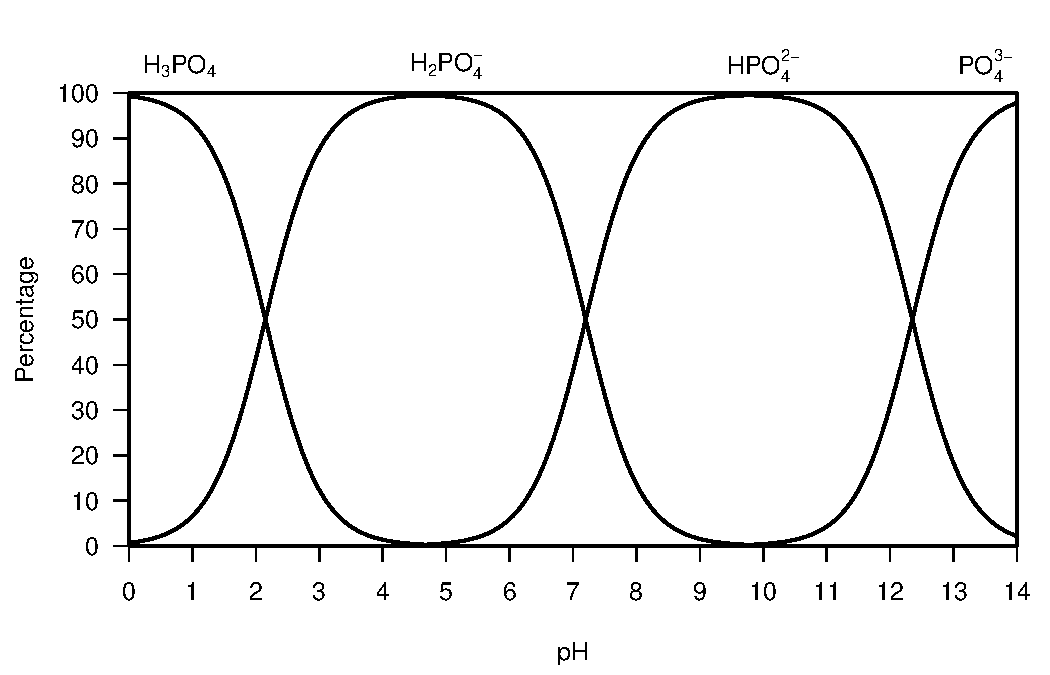
\includegraphics[keepaspectratio]{Thesis_files/figure-pdf/fig-phosphate-speciation-tight-1.pdf}}

}

\caption{\label{fig-phosphate-speciation-tight}Phosphate speciation
(percent) as a function of pH.}

\end{figure}%

From a causal-inference perspective, identification of an effect
requires isolating variation in a target factor while holding other
causally relevant factors fixed or blocked (ceteris paribus). In plant
nutrition experiments, strict independent variation of a single ionic
species is generally not possible, because electroneutrality and
acid--base equilibria couple ionic charge, pH, ionic strength and
osmotic potential. As a result, strict ceteris paribus conditions for
individual ions cannot be achieved in bulk nutrient solutions; they can
only be approximated within constrained experimental frameworks. Within
this framework, classical experimental designs in plant nutrition can be
derived as three distinct classes of experiments, defined by the
invariants they preserve in meq-space.

Here, \(\Delta\) denotes the change induced by the experimental
manipulation,
i.e.~\(\Delta x := x_{\text{treatment}} - x_{\text{control}}\) (or, more
generally, the difference between two solution states). The first class
consists of qualitative, or ion-substitution, experiments. In these
experiments, one ionic species is replaced by another while total cation
and total anion charge equivalents are kept constant:

\begin{align*}
\Delta \mathrm{meq}_i + \Delta \mathrm{meq}_j &= 0 .
\end{align*}

When the substituted ions have the same charge, the substitution is
isovalent (e.g.~\(\mathrm{K^+} \leftrightarrow \mathrm{Na^+}\) or
\(\mathrm{Cl^-} \leftrightarrow \mathrm{NO_3^-}\)). When the charges
differ, the substitution is heterovalent, for example replacing \(2\)
meq of \(\mathrm{K^+}\) (2 mmol) with \(2\) meq of \(\mathrm{Ca^{2+}}\)
(1 mmol). Qualitative substitution experiments provide the highest
degree of causal specificity achievable within whole-solution
manipulations at fixed charge totals, although their interpretation
remains conditional on buffering and counter-ion choice.

The second class comprises quantitative, or salt addition (or removal),
experiments. Here, the total amount of dissolved salt is changed, which
necessarily alters both total cation and total anion charge equivalents
by the same non-zero amount:

\begin{align*}
\Delta \sum \mathrm{meq}_{\text{cat}}
&= \Delta \sum \mathrm{meq}_{\text{an}}
\neq 0 .
\end{align*}

Electroneutrality is preserved automatically, but ionic strength,
electrical conductivity and osmotic potential change and pH may shift
depending on buffering. Because at least two ionic components vary
simultaneously, plant responses in such experiments reflect composite
effects of nutrient ions, counter-ions and general salinity.

The third class treats quantity as an emergent quality through
solution-strength series. In this case, all charge equivalents in the
solution are scaled by a constant factor \(k\):

\begin{align*}
\mathbf{S}_{\mathrm{meq},k}
&= k\, \mathbf{S}_{\mathrm{meq},1} .
\end{align*}

This transformation preserves ion ratios expressed in meq while
increasing or decreasing total charge density, ionic strength and
osmotic potential. Although composition remains constant at the level of
charge ratios, pH and ionic speciation may shift because acid--base
equilibria are nonlinear. As a result, solution strength functions as an
environmental condition rather than a simple quantitative variable.

Across these three experiment types, causal specificity for individual
ion identity typically decreases as the number of inseparable or
uncontrolled variables increases. Qualitative substitution experiments
offer the highest degree of causal specificity, whereas quantitative
salt manipulations and solution-strength series progressively trade
causal resolution for ecological or agronomic relevance. These
experiment classes are therefore best understood as distinct projections
of a chemically constrained ionic system, most transparently described
in milliequivalent space.

From a plant nutrition perspective, comparisons between nutrient
solutions of different provenance are only informative to the extent
that differences in ionic composition are maintained or eliminated in a
controlled manner. If two solutions of different origin, such as
wastewater-derived (e.g.~animal or human urine) and mineral solutions,
are formulated to the same ionic composition, then the specifically
nutritional dimension of the comparison is largely removed, reducing the
question to a Ship of Theseus problem of identity. Under such
conditions, any remaining differences are more appropriately interpreted
in terms of economic factors associated with source, production,
transport, cost and sustainability rather than nutrient composition
itself.

\begin{landscape}
\begingroup
\fontsize{11}{13}\selectfont
\setlength{\tabcolsep}{4pt}
\renewcommand{\arraystretch}{1.1}

\begin{tabular}{
>{\raggedright\arraybackslash}p{2.8cm}
>{\raggedright\arraybackslash}p{3.2cm}
>{\raggedright\arraybackslash}p{4.2cm}
>{\raggedright\arraybackslash}p{3.2cm}
>{\raggedright\arraybackslash}p{4.0cm}
>{\raggedright\arraybackslash}p{2.7cm}
>{\raggedright\arraybackslash}p{3.2cm}
}
\toprule
Experiment class & Core manipulation & Charge balance condition & Held constant & Necessarily changes & Example & Interpretation \\
\midrule
I.a Qualitative (isovalent) &
Equal-meq substitution &
$\begin{aligned}
\Delta \sum \mathrm{meq}_{cat} &= 0 \\
\Delta \sum \mathrm{meq}_{an}  &= 0
\end{aligned}$ &
Total cation \& anion meq &
Ion identity &
$\mathrm{K^+}\!\leftrightarrow\!\mathrm{Na^+}$ &
Conditional ion identity effect \\
\addlinespace[3pt]
I.b Qualitative (heterovalent) &
Equal-meq substitution &
$\Delta \mathrm{meq}_i+\Delta \mathrm{meq}_j=0$ &
Charge equivalents &
Molar conc., ionic strength &
$2$ mmol $\mathrm{K^+}\!\leftrightarrow\!1$ mmol $\mathrm{Ca^{2+}}$ &
Identity + secondary effects \\
\addlinespace[3pt]
II Quantitative &
Salt addition or removal &
$\begin{aligned}
\Delta \sum \mathrm{meq}_{cat} &= \\ \Delta \sum \mathrm{meq}_{an} 
&\neq 0
\end{aligned}$ &
Electroneutrality &
Ions, EC, osmotic potential &
$\uparrow\,\mathrm{KCl}$ &
Composite salt effect \\
\addlinespace[3pt]
III Quantitative-as-qualitative &
Solution scaling &
$\mathbf{S}_{\mathrm{meq},k}=k\,\mathbf{S}_{\mathrm{meq},1}$ &
meq ratios &
Total charge, speciation &
¼×, ½×, 1× &
Environmental strength effect \\
\bottomrule
\end{tabular}

\endgroup
\end{landscape}

\section{Stoichiometry and salt--ion
relationships}\label{stoichiometry-and-saltion-relationships}

In hydroponics, nutrients are supplied by dissolving fertilizer salts in
water to prepare a nutrient solution (Resh, 2013). The formulation of
such solutions is complicated by the declaration conventions used for
commercial fertilizers. Nutrient contents are commonly expressed in
oxide form rather than as elemental concentrations or ionic species.
Thus, potassium is typically declared as K₂O rather than as K or ionic
K⁺, while phosphorus is conventionally declared as P₂O₅ rather than as P
or as the pH-dependent phosphate species H₂PO₄⁻, HPO₄²⁻, or PO₄³⁻.
Although these conventions are historically established, they introduce
an unnecessary level of abstraction and increase the susceptibility of
nutrient calculations to error.

A more serious limitation is that fertilizer labels do not necessarily
disclose all contained elements. As a result, attempts to recalculate
complete fertilizer compositions in ionic form often fail to account for
100 \% of the product mass. One reason is that elements such as chloride
may be present without mandatory declaration. Under Regulation (EC) No
2003/2003, only specific nutrient categories are subject to declaration
requirements, namely the primary nutrients nitrogen, phosphorus and
potassium; the secondary nutrients calcium, magnesium, sodium and
sulfur; and the micronutrients boron, cobalt, copper, iron, manganese,
molybdenum and zinc. In addition, secondary nutrients must only be
declared above specified threshold concentrations. For sodium, for
example, declaration is required only above 3 \% Na₂O or 2.2 \% Na.

For this reason, the present work was restricted to single salts or
mixtures of single salts with chemically defined composition. Such
compounds can be represented directly by their molecular formulas, so
that molar mass and stoichiometric composition are fully determined by
the sum of the constituent elements and their stoichiometric
coefficients. This ensures complete compositional transparency and
avoids the uncertainty associated with incomplete commercial fertilizer
declarations.

Many fertilizers used in greenhouse production are in fact single salts.
A representative example is Epsom salt, MgSO₄·7H₂O, marketed by Yara as
YaraTera KRISTA MgS and declared as containing 16 \% MgO and 32.5 \% SO₃
(YARA, 2026). Chemically, pure MgSO₄·7H₂O contains 9.86 \% Mg and 13.01
\% S, corresponding to 16.35 \% MgO and 32.48 \% SO₃, or 38.98 \% SO₄.
Thus, 51.16 \% of the compound mass consists of water of
crystallization. Another example is calcium nitrate, which may occur as
anhydrous Ca(NO₃)₂, as the hydrate Ca(NO₃)₂·4H₂O, or as the double salt
5Ca(NO₃)₂·NH₄NO₃·10H₂O. These distinctions are stoichiometrically
relevant because each form differs in molar mass and nutrient
contribution, even where the commercial designation is similar.

\section{Existing tools}\label{existing-tools}

A classical approach to nutrient-solution calculation is the universal
algorithm proposed by Sonneveld et al. (1999). The method follows an
iterative balancing procedure in which fertilizer salts are added
stepwise to meet nutrient targets, while the residual nutrient
requirements are recalculated after each addition because each salt
simultaneously contributes several ions. In this way, the final
formulation is obtained through successive correction of remaining
deficits under the constraints imposed by salt composition, target EC
and raw-water composition.

Nutrient Solution Calculator is an Excel™-based tool developed by Luca
Incrocci and supported by the EUPHOROS project (Pardossi et al., 2011).
It was previously available for download via Wageningen University and
was still accessible in 2024, but was no longer publicly available there
in 2026 (Incrocci, 2007). A Spanish translation remains available online
through the University of Almeria (Incrocci et al., 2020). The
spreadsheet is designed to calculate the composition and cost of
fertigation stock solutions (A+B) from three principal inputs: the ionic
composition of the irrigation water, the crop nutrient recipe, including
target pH, EC and nutrient concentrations and the technical
characteristics of the fertigation system, particularly stock tank
volume and dilution ratio. Furthermore, it evaluates the potential risk
of salt precipitation in concentrated stock solutions. The spreadsheet
is password-protected.

Another tool is HydroBuddy, a free and open-source software application
developed by Daniel Fernández Pinto for the formulation of hydroponic
nutrient solutions (Fernández Pinto, 2022). The program calculates the
required quantities of fertilizers to achieve specified target nutrient
concentrations. It includes a database of commonly used fertilizers
whose compositions can be edited or extended by the user and allows the
formulation of both direct nutrient solutions and concentrated stock
solutions. The software determines the combination of fertilizer salts
that best matches the desired nutrient composition through the solution
of a system of linear equations and also provides an empirical
estimation of the EC.

At present, no dedicated open-source R library is available for
transparent, modular nutrient-solution calculation in horticultural
applications.

\chapter{Material and Methods}\label{material-and-methods}

The development of the computational framework followed a structured
development and validation pipeline. The R package was developed using
the devtools package (Wickham et al., 2025). The first step involved
designing the underlying data structures. A compound-by-nutrient matrix
was established in which rows represented fertilizer compounds (salts)
and columns represented nutrients such as N, P, K and Ca. For solving,
this matrix was transposed internally so that nutrient equations formed
the rows used by the NNLS routine. Each fertilizer was parsed on the
basis of its molecular formula into its elemental components using a
database of molar masses and established stoichiometric rules.

Building on this foundation, an R package was developed. The package
includes core functions for parsing chemical formulas and computing
molar masses, as well as for converting between different chemical
representations such as oxides and elemental forms (e.g., P₂O₅ to P or
SO₄ to S). It also includes tools for transforming concentration units
(e.g., from mmol L⁻¹ to mg L⁻¹) using accurate molar-mass calculations.
In addition, bidirectional transformations between compound-based and
elemental quantities were integrated on the basis of stoichiometric
relationships.

The central component of the package was the implementation of the
nutrient-solution formulation algorithm. This algorithm used
nnls::nnls() to solve the system of equations under non-negativity
constraints and to quantify deviations between the target and calculated
solution in terms of absolute and relative error. The framework also
allows users to assign weights to individual nutrients, thereby enabling
the exploration of different formulation priorities and trade-offs.

The framework was validated through a series of use cases. These
included reproducing historical and crop-specific nutrient solutions,
comparing the computed results with values reported in the literature
and compiling crop- and author-specific nutrient solutions into a base
library. The distribution of anions and cations across different
solutions was visualized, for example, by ternary plots for cations (K⁺,
Ca²⁺, Mg²⁺) and anions (NO₃⁻, SO₄²⁻, PO₄³⁻), in order to classify
nutrient combinations systematically, as proposed by Steiner (1961).

\section{Software Environment and Data
Sources}\label{software-environment-and-data-sources}

\subsection{R version, packages}\label{r-version-packages}

The package \texttt{nutricalc} was written in R 4.5.1 (R Core Team,
2025) using Posit RStudio 2025.09.2+418 ``Cucumberleaf Sunflower''
(Posit team, 2025). Following packages were used: \texttt{stringr}
(Wickham et al., 2025), \texttt{nnls} (Mullen \& van Stokkum, 2024),
\texttt{shiny} (Chang et al., 2025), \texttt{bslib} (Sievert et al.,
2025), \texttt{Ternary} (Smith \& Sanselme, 2025), \texttt{xml2}
(Wickham et al., 2026). For the development in R \texttt{devtools}
(Wickham, 2025) was used.

Code of the package is provided on GitHub under
\url{https://github.com/diolsa/nutricalc} and the shiny-App is deployed
under: \url{https://nutricalc.shinyapps.io/nutricalc-app/}

Code development was supported by AI-assisted LLM for debugging and
optimization to ensure code quality and computational reliability with
OpenAI CODEX and ChatGPT 5.2.

\subsection{Built-in recipe datasets}\label{built-in-recipe-datasets}

Hewitt (1966) compiled a large proportion of the nutrient-solution
formulations used during the first half of the twentieth century. For
the present work, selected standard recipes from this compilation were
considered, particularly those that remain relevant in contemporary
research and horticultural practice. In addition, 38 crop-specific
horticultural recipes from Sonneveld \& Straver (1994) were included.
These recipes were assigned to the three groups \texttt{Olericulture},
\texttt{Floriculture} and \texttt{Fruticulture}. In the original source,
Sonneveld \& Straver (1994) also classified the formulations into the
categories \texttt{A}, \texttt{B} and \texttt{C}, reflecting their
practical and experimental suitability for the respective crop. The
resulting set of formulations is shown in
Table~\ref{tbl-crop-recipes-long-landscape_units}.

\setlength{\LTpre}{-10pt}
\setlength{\LTpost}{0pt}
\renewcommand{\arraystretch}{0.85}

\begin{landscape}\begingroup\fontsize{7}{9}\selectfont

\begin{longtable}[t]{llcccccccccccccc}

\caption{\label{tbl-crop-recipes-long-landscape_units}Target
compositions of crop-specific nutrient solutions (Olericulture,
Floriculture, Fruticulture) from Sonneveld \& Straver (1994)}

\tabularnewline

\\
\toprule
\multicolumn{2}{c}{ } & \multicolumn{7}{c}{mmol~L⁻¹} & \multicolumn{7}{c}{µmol~L⁻¹} \\
\cmidrule(l{3pt}r{3pt}){3-9} \cmidrule(l{3pt}r{3pt}){10-16}
Category & Recipe & NO₃–N & NH₄–N & P & K & Ca & Mg & S & Fe & Mn & Zn & B & Cu & Mo & Si\\
\midrule
\endfirsthead
\caption[]{Target compositions of crop-specific nutrient solutions (Olericulture, Floriculture, Fruticulture) from @Sonneveld.1994 \textit{(continued)}}\\
\toprule
\multicolumn{2}{c}{ } & \multicolumn{7}{c}{mmol~L⁻¹} & \multicolumn{7}{c}{µmol~L⁻¹} \\
\cmidrule(l{3pt}r{3pt}){3-9} \cmidrule(l{3pt}r{3pt}){10-16}
Category & Recipe & NO₃–N & NH₄–N & P & K & Ca & Mg & S & Fe & Mn & Zn & B & Cu & Mo & Si\\
\midrule
\endhead

\endfoot
\bottomrule
\endlastfoot
 & Endive in Recirculating Water & 19 & 1.25 & 2 & 9 & 5 & 1.5 & 1.125 & 40 & 5 & 4 & 30 & 0.75 & 0.5 & 0\\
\nopagebreak
 & Eggplant in Rockwool & 15.5 & 1.5 & 1.25 & 6.75 & 3.25 & 2.5 & 1.5 & 15 & 10 & 5 & 30 & 0.75 & 0.5 & 0\\
\nopagebreak
 & Eggplant in Rockwool (RDW) & 11.75 & 1 & 1 & 6.5 & 2.25 & 1.5 & 1.125 & 15 & 10 & 5 & 20 & 0.75 & 0.5 & 0\\
\nopagebreak
 & Bean in Rockwool & 12 & 1 & 1.25 & 5.5 & 3.25 & 1.25 & 1.125 & 10 & 10 & 4 & 20 & 0.5 & 0.5 & 0\\
\nopagebreak
 & Courgette in Rockwool & 16 & 1.25 & 1.25 & 7.25 & 3.625 & 2 & 1.25 & 10 & 10 & 5 & 30 & 0.75 & 0.5 & 0\\
\nopagebreak
 & Cucumber in Rockwool & 16 & 1.25 & 1.25 & 8 & 4 & 1.375 & 1.375 & 15 & 10 & 5 & 25 & 0.75 & 0.5 & 750\\
\nopagebreak
 & Cucumber in Rockwool (RDW) & 11.75 & 1 & 1.25 & 6.5 & 2.75 & 1 & 1 & 15 & 10 & 5 & 25 & 0.75 & 0.5 & 750\\
\nopagebreak
 & Propagation vegetable plants in rockwool & 16.75 & 1.25 & 1.25 & 6.75 & 4.5 & 3 & 2.5 & 25 & 10 & 5 & 35 & 1 & 0.5 & 0\\
\nopagebreak
 & Sweet Pepper in Rockwool & 15.5 & 1.25 & 1.25 & 6.5 & 4.75 & 1.5 & 1.75 & 15 & 10 & 5 & 30 & 0.75 & 0.5 & 0\\
\nopagebreak
 & Sweet Pepper in Rockwool (RDW) & 12.75 & 1.25 & 1 & 5.75 & 3.25 & 1.125 & 1 & 15 & 10 & 4 & 25 & 0.75 & 0.5 & 0\\
\nopagebreak
 & Lettuce in Recirculating Water & 19 & 1.25 & 2 & 11 & 4.5 & 1 & 1.125 & 40 & 5 & 4 & 30 & 0.75 & 0.5 & 500\\
\nopagebreak
 & Tomato in Rockwool & 13.75 & 1.25 & 1.25 & 8.75 & 4.25 & 2 & 3.75 & 15 & 10 & 5 & 30 & 0.75 & 0.5 & 0\\
\nopagebreak
\multirow[t]{-13}{*}{\raggedright\arraybackslash Olericulture} & Tomato in Rockwool (RDW) & 10.75 & 1 & 1.25 & 6.5 & 2.75 & 1 & 1.5 & 15 & 10 & 4 & 20 & 0.75 & 0.5 & 0\\
\cmidrule{1-16}\pagebreak[0]
 & Alstroemeria in Rockwool & 11.25 & 1.25 & 1.25 & 6 & 2.875 & 1 & 1.25 & 25 & 10 & 4 & 25 & 0.75 & 0.5 & 0\\
\nopagebreak
 & Alstroemeria in Rockwool (RDW) & 7.5 & 0.75 & 1 & 4.75 & 2 & 0.75 & 1.25 & 25 & 5 & 4 & 20 & 0.75 & 0.5 & 0\\
\nopagebreak
 & Anemone in Rockwool & 13 & 1 & 1.5 & 6.5 & 3.75 & 1 & 1.25 & 35 & 5 & 4 & 30 & 0.75 & 0.5 & 0\\
\nopagebreak
 & Carnation in Rockwool or Peat & 13 & 1 & 1.25 & 6.25 & 3.75 & 1 & 1.25 & 25 & 10 & 4 & 30 & 0.75 & 0.5 & 0\\
\nopagebreak
 & Carnation in Rockwool (reuse drainage) & 7 & 0.75 & 0.8 & 4 & 1.625 & 0.6 & 0.7 & 20 & 5 & 3 & 20 & 0.5 & 0.5 & 0\\
\nopagebreak
 & Anthurium andreanum in Rockwool or Peat & 4.5 & 0.8 & 0.7 & 3 & 1 & 0.7 & 1 & 15 & 3 & 3 & 20 & 0.5 & 0.5 & 0\\
\nopagebreak
 & Aster in Rockwool or Peat & 13 & 1 & 1.25 & 6.25 & 3.75 & 1 & 1.25 & 25 & 10 & 4 & 30 & 0.75 & 0.5 & 0\\
\nopagebreak
 & Bouvardia in Rockwool & 13 & 1.25 & 1.75 & 6 & 4.25 & 1 & 1.5 & 25 & 5 & 3.5 & 20 & 0.75 & 0.5 & 0\\
\nopagebreak
 & Bouvardia in Rockwool (RDW) & 8 & 1 & 1.5 & 4 & 2.5 & 0.5 & 0.75 & 25 & 5 & 3.5 & 20 & 0.75 & 0.5 & 0\\
\nopagebreak
 & Chrysanthemum in Recirculating Water & 12.75 & 1.25 & 1 & 7.5 & 2.5 & 1 & 1 & 60 & 20 & 3 & 20 & 0.5 & 0.5 & 0\\
\nopagebreak
 & Cymbidium in phenol foam & 4.5 & 0.5 & 0.8 & 3 & 1.2 & 0.75 & 1.05 & 8 & 10 & 4 & 20 & 0.4 & 0.4 & 0\\
\nopagebreak
 & Cymbidium in rockwool/urethane foam & 4 & 1 & 0.8 & 2.8 & 1 & 0.75 & 1.25 & 8 & 10 & 4 & 20 & 0.4 & 0.4 & 0\\
\nopagebreak
 & Euphorbia fulgens in Rockwool & 11.5 & 1 & 1.5 & 6 & 3.5 & 1 & 1.5 & 35 & 10 & 3 & 20 & 0.5 & 0.5 & 0\\
\nopagebreak
 & Freesia in Rockwool or Sand & 14.5 & 1.25 & 1.25 & 7.75 & 3.375 & 1.5 & 1.5 & 25 & 10 & 4 & 25 & 0.75 & 0.5 & 0\\
\nopagebreak
 & Gerbera in Rockwool & 11.25 & 1.5 & 1.25 & 5.5 & 3 & 1 & 1.25 & 35 & 5 & 4 & 30 & 0.75 & 0.5 & 0\\
\nopagebreak
 & Gerbera in Rockwool (RDW) & 7.25 & 0.75 & 0.6 & 4.5 & 1.6 & 0.4 & 0.7 & 25 & 5 & 3 & 20 & 0.5 & 0.5 & 0\\
\nopagebreak
 & Gypsophila in Rockwool & 17 & 1.25 & 1.25 & 4 & 6 & 1.7 & 1.2 & 25 & 10 & 4 & 30 & 0.8 & 0.5 & 0\\
\nopagebreak
 & Hippeastrum in Pumice & 13 & 1 & 1.25 & 7.5 & 3.125 & 1 & 1.25 & 10 & 10 & 5 & 30 & 0.5 & 0.5 & 0\\
\nopagebreak
 & Pot Plants in Expanded Clay & 10.6 & 1.1 & 1.5 & 5.5 & 3 & 0.75 & 1 & 20 & 10 & 3 & 20 & 0.5 & 0.5 & 0\\
\nopagebreak
 & Rose in Rockwool & 11 & 1.5 & 1.25 & 4.5 & 3.25 & 1.125 & 1.25 & 25 & 5 & 3.5 & 20 & 0.75 & 0.5 & 0\\
\nopagebreak
 & Rose in Rockwool (RDW) & 4.3 & 0.85 & 0.5 & 2.15 & 0.9 & 0.5 & 0.5 & 15 & 5 & 3 & 15 & 0.5 & 0.5 & 0\\
\nopagebreak
\multirow[t]{-22}{*}{\raggedright\arraybackslash Floriculture} & Statice in Rockwool & 12 & 1 & 1 & 6 & 3 & 1 & 1 & 15 & 10 & 5 & 2.5 & 0.75 & 0.5 & 0\\
\cmidrule{1-16}\pagebreak[0]
 & Strawberry in Peaty Substrates & 11.5 & 1 & 1 & 5.5 & 3.25 & 1.25 & 1.5 & 20 & 10 & 7 & 25 & 0.75 & 0.5 & 0\\
\nopagebreak
 & Strawberry in Recirculating Water & 10 & 0.5 & 1.25 & 5.25 & 2.75 & 1.125 & 1.125 & 20 & 10 & 4 & 20 & 0.75 & 0.5 & 0\\
\nopagebreak
\multirow[t]{-3}{*}{\raggedright\arraybackslash Fruticulture} & Melon in Rockwool & 16.25 & 1 & 1.25 & 7.5 & 4.75 & 1.25 & 1.5 & 10 & 10 & 4 & 20 & 0.5 & 0.5 & 750\\*

\end{longtable}

\endgroup{}
\end{landscape}
\renewcommand{\arraystretch}{1}

\section{Data Structures and Chemical
Representation}\label{data-structures-and-chemical-representation}

\subsection{Elementary Entities}\label{elementary-entities}

After the 2019 revision of the International System of Units, the base
units are defined by fixed numerical values of fundamental constants
(BIPM, 2019). The mole is the SI unit for the amount of a substance; its
symbol is mol. The defining constant is the Avogadro constant,
N\textsubscript{A} Thus:

\begin{equation} 1\,\mathrm{mol} = 6.02214076 \times 10^{23}\,\text{elementary entities} \end{equation}

An elementary entity may be an atom, a molecule, or any other particle.
In this work, the elementary entities are ions, as listed in Table
\ref{tab:element-molar-mass}. The molar masses were taken from the CRC
Handbook of Chemistry and Physics (Haynes, 2017) and rounded to three
decimal places. Not all listed elements are essential for plant
nutrition. The set also includes non-essential and potentially toxic
elements that may occur in the plant ionome or in fertilizers and source
water, although not all of these elements were incorporated into the
final framework.

\par

\noindent \begingroup \footnotesize \noindent\makebox[\linewidth][c]{%
\begin{minipage}{\minof{\linewidth}{\widthof{
\begin{tabular}{llr}
\toprule
Symbol & Element name & Molar Mass [$\mathrm{g\,mol^{-1}}$]\\
\midrule
C & Carbon & 12.011\\
O & Oxygen & 15.999\\
H & Hydrogen & 1.008\\
N & Nitrogen & 14.007\\
P & Phosphorus & 30.974\\
\addlinespace
K & Potassium & 39.098\\
Mg & Magnesium & 24.305\\
S & Sulfur & 32.065\\
Ca & Calcium & 40.078\\
B & Boron & 10.811\\
\addlinespace
Cu & Copper & 63.546\\
Cl & Chlorine & 35.453\\
Fe & Iron & 55.845\\
Mn & Manganese & 54.938\\
Ni & Nickel & 58.693\\
\addlinespace
Zn & Zinc & 65.380\\
Mo & Molybdenum & 95.950\\
Na & Sodium & 22.990\\
Al & Aluminum & 26.982\\
Co & Cobalt & 58.933\\
\addlinespace
Se & Selenium & 78.971\\
Si & Silicon & 28.085\\
\bottomrule
\end{tabular}}}}
\captionsetup{format=plain,labelsep=colon,labelfont=bf,justification=raggedright,singlelinecheck=false,skip=4pt}
\captionof{table}{Molar masses of elementary entities used for nutrient formulation.}\label{tab:element-molar-mass}

\begin{tabular}{llr}
\toprule
Symbol & Element name & Molar Mass [$\mathrm{g\,mol^{-1}}$]\\
\midrule
C & Carbon & 12.011\\
O & Oxygen & 15.999\\
H & Hydrogen & 1.008\\
N & Nitrogen & 14.007\\
P & Phosphorus & 30.974\\
\addlinespace
K & Potassium & 39.098\\
Mg & Magnesium & 24.305\\
S & Sulfur & 32.065\\
Ca & Calcium & 40.078\\
B & Boron & 10.811\\
\addlinespace
Cu & Copper & 63.546\\
Cl & Chlorine & 35.453\\
Fe & Iron & 55.845\\
Mn & Manganese & 54.938\\
Ni & Nickel & 58.693\\
\addlinespace
Zn & Zinc & 65.380\\
Mo & Molybdenum & 95.950\\
Na & Sodium & 22.990\\
Al & Aluminum & 26.982\\
Co & Cobalt & 58.933\\
\addlinespace
Se & Selenium & 78.971\\
Si & Silicon & 28.085\\
\bottomrule
\end{tabular}
\end{minipage}} \endgroup

\par

\subsection{Fertilizer inventory}\label{fertilizer-inventory}

Table \ref{tab:salt-molar-mass} lists the 40 fertilizer compounds
implemented in the solver, including their chemical formulas, compound
names,and calculated molar masses. The molar mass of each compound was
calculated from its chemical formula using the molar masses of the
constituent elements and their stoichiometric coefficients reported in
Table \ref{tab:element-molar-mass}.

\par

\noindent \begingroup \footnotesize \noindent\makebox[\linewidth][c]{%
\begin{minipage}{\minof{\linewidth}{\widthof{
\begin{tabular}{llr}
\toprule
Formula & Name & Molar mass [g mol\textsuperscript{-1}]\\
\midrule
\ce{NH4Cl} & Ammonium chloride & 53.492\\
\ce{NH4H2PO4} & Ammonium dihydrogen phosphate & 115.025\\
\ce{((NH4)6)Mo7O24*4H2O} & Ammonium heptamolybdate tetrahydrate & 1235.920\\
\ce{NH4OH} & Ammonium hydroxide & 35.046\\
\ce{NH4NO3} & Ammonium nitrate & 80.043\\
\addlinespace
\ce{(NH4)2SO4} & Ammonium sulfate & 132.139\\
\ce{H3BO3} & Boric acid & 61.832\\
\ce{CaCl2*2H2O} & Calcium chloride dihydrate & 147.014\\
\ce{Ca(OH)2} & Calcium hydroxide & 74.092\\
\ce{Ca(NO3)2} & Calcium nitrate & 164.086\\
\addlinespace
\ce{Ca(NO3)2*4H2O} & Calcium nitrate tetrahydrate & 236.146\\
\ce{5Ca(NO3)2*NH4NO3*10H2O} & Calcium nitrate–ammonium nitrate decahydrate (5:1) & 1080.623\\
\ce{CaSO4*2H2O} & Calcium sulfate dihydrate & 172.169\\
\ce{CuCl2} & Copper(II) chloride & 134.452\\
\ce{CuSO4*5H2O} & Copper(II) sulfate pentahydrate & 249.682\\
\addlinespace
\ce{(NH4)2HPO4} & Diammonium hydrogen phosphate & 132.056\\
\ce{HCl} & Hydrochloric acid & 36.461\\
\ce{C18H16N2O6FeNa} & Iron(III) sodium EDDHA & 435.169\\
\ce{C10H12N2O8FeNa*3H2O} & Iron(III) sodium EDTA trihydrate & 421.092\\
\ce{Mg(NO3)2*6H2O} & Magnesium nitrate hexahydrate & 256.403\\
\addlinespace
\ce{MgSO4*7H2O} & Magnesium sulfate heptahydrate & 246.471\\
\ce{MnCl2*4H2O} & Manganese(II) chloride tetrahydrate & 197.904\\
\ce{MnSO4*H2O} & Manganese(II) sulfate monohydrate & 169.014\\
\ce{KH2PO4} & Monopotassium dihydrogen phosphate & 136.084\\
\ce{HNO3} & Nitric acid & 63.012\\
\addlinespace
\ce{H3PO4} & Phosphoric acid & 97.994\\
\ce{KCl} & Potassium chloride & 74.551\\
\ce{KOH} & Potassium hydroxide & 56.105\\
\ce{KNO3} & Potassium nitrate & 101.102\\
\ce{K2SiO3} & Potassium silicate & 154.278\\
\addlinespace
\ce{K2SO4} & Potassium sulfate & 174.257\\
\ce{NaCl} & Sodium chloride & 58.443\\
\ce{NaOH} & Sodium hydroxide & 39.997\\
\ce{Na2MoO4*2H2O} & Sodium molybdate dihydrate & 241.956\\
\ce{NaNO3} & Sodium nitrate & 84.994\\
\addlinespace
\ce{Na2B4O7*10H2O} & Sodium tetraborate decahydrate (borax) & 381.367\\
\ce{H2SO4} & Sulfuric acid & 98.077\\
\ce{ZnCl2} & Zinc chloride & 136.286\\
\ce{ZnSO4*7H2O} & Zinc sulfate heptahydrate & 287.546\\
\ce{ZnSO4*6H2O} & Zinc sulfate hexahydrate & 269.531\\
\bottomrule
\end{tabular}}}}
\captionsetup{format=plain,labelsep=colon,labelfont=bf,justification=raggedright,singlelinecheck=false,skip=4pt}
\captionof{table}{Fertilizer compounds and their molar masses.}\label{tab:salt-molar-mass}

\begin{tabular}{llr}
\toprule
Formula & Name & Molar mass [g mol\textsuperscript{-1}]\\
\midrule
\ce{NH4Cl} & Ammonium chloride & 53.492\\
\ce{NH4H2PO4} & Ammonium dihydrogen phosphate & 115.025\\
\ce{((NH4)6)Mo7O24*4H2O} & Ammonium heptamolybdate tetrahydrate & 1235.920\\
\ce{NH4OH} & Ammonium hydroxide & 35.046\\
\ce{NH4NO3} & Ammonium nitrate & 80.043\\
\addlinespace
\ce{(NH4)2SO4} & Ammonium sulfate & 132.139\\
\ce{H3BO3} & Boric acid & 61.832\\
\ce{CaCl2*2H2O} & Calcium chloride dihydrate & 147.014\\
\ce{Ca(OH)2} & Calcium hydroxide & 74.092\\
\ce{Ca(NO3)2} & Calcium nitrate & 164.086\\
\addlinespace
\ce{Ca(NO3)2*4H2O} & Calcium nitrate tetrahydrate & 236.146\\
\ce{5Ca(NO3)2*NH4NO3*10H2O} & Calcium nitrate–ammonium nitrate decahydrate (5:1) & 1080.623\\
\ce{CaSO4*2H2O} & Calcium sulfate dihydrate & 172.169\\
\ce{CuCl2} & Copper(II) chloride & 134.452\\
\ce{CuSO4*5H2O} & Copper(II) sulfate pentahydrate & 249.682\\
\addlinespace
\ce{(NH4)2HPO4} & Diammonium hydrogen phosphate & 132.056\\
\ce{HCl} & Hydrochloric acid & 36.461\\
\ce{C18H16N2O6FeNa} & Iron(III) sodium EDDHA & 435.169\\
\ce{C10H12N2O8FeNa*3H2O} & Iron(III) sodium EDTA trihydrate & 421.092\\
\ce{Mg(NO3)2*6H2O} & Magnesium nitrate hexahydrate & 256.403\\
\addlinespace
\ce{MgSO4*7H2O} & Magnesium sulfate heptahydrate & 246.471\\
\ce{MnCl2*4H2O} & Manganese(II) chloride tetrahydrate & 197.904\\
\ce{MnSO4*H2O} & Manganese(II) sulfate monohydrate & 169.014\\
\ce{KH2PO4} & Monopotassium dihydrogen phosphate & 136.084\\
\ce{HNO3} & Nitric acid & 63.012\\
\addlinespace
\ce{H3PO4} & Phosphoric acid & 97.994\\
\ce{KCl} & Potassium chloride & 74.551\\
\ce{KOH} & Potassium hydroxide & 56.105\\
\ce{KNO3} & Potassium nitrate & 101.102\\
\ce{K2SiO3} & Potassium silicate & 154.278\\
\addlinespace
\ce{K2SO4} & Potassium sulfate & 174.257\\
\ce{NaCl} & Sodium chloride & 58.443\\
\ce{NaOH} & Sodium hydroxide & 39.997\\
\ce{Na2MoO4*2H2O} & Sodium molybdate dihydrate & 241.956\\
\ce{NaNO3} & Sodium nitrate & 84.994\\
\addlinespace
\ce{Na2B4O7*10H2O} & Sodium tetraborate decahydrate (borax) & 381.367\\
\ce{H2SO4} & Sulfuric acid & 98.077\\
\ce{ZnCl2} & Zinc chloride & 136.286\\
\ce{ZnSO4*7H2O} & Zinc sulfate heptahydrate & 287.546\\
\ce{ZnSO4*6H2O} & Zinc sulfate hexahydrate & 269.531\\
\bottomrule
\end{tabular}
\end{minipage}} \endgroup

\par

\subsection{Compound-by-nutrient
matrix}\label{compound-by-nutrient-matrix}

Table \ref{tab:nutrient-matrix-no-chelate} shows the
compound-by-nutrient matrix, listing the amount of each nutrient in mmol
provided per mmol of compound for all 40 fertilizers. The table is
organised with the chemical formula of each compound in the first
column, followed by a column indicating the solver stage (1 for salts, 2
for acids and bases) and then columns for each nutrient. Chelates are
also part of the full matrix, but are excluded from the table shown here
for better readability. Each compound is additionally linked to metadata
such as compound name, category and acid/base status.

\par

\noindent \begingroup \scriptsize \setlength{\tabcolsep}{3pt}
\renewcommand{\arraystretch}{0.9} \noindent\makebox[\linewidth][c]{%
\begin{minipage}{\linewidth}
\captionsetup{format=plain,labelsep=colon,labelfont=bf,justification=raggedright,singlelinecheck=false,skip=4pt}
\captionof{table}{Compound--nutrient stoichiometric matrix (mmol nutrient per mmol compound). Stage 1 = salts, Stage 2 = acids/bases.}\label{tab:nutrient-matrix-no-chelate}
\resizebox{\linewidth}{!}{%

\begin{tabular}{lrrrrrrrrrrrrrrrrr}
\toprule
Formula & Solver & NO3\_N & NH4\_N & P & K & Ca & Mg & S & Na & Cl & Fe & Mn & Zn & B & Cu & Mo & Si\\
\midrule
\ce{Ca(NO3)2} & 1 & 2 & 0 & 0 & 0 & 1 & 0 & 0 & 0 & 0 & 0 & 0 & 0 & 0 & 0 & 0 & 0\\
\ce{NH4NO3} & 1 & 1 & 1 & 0 & 0 & 0 & 0 & 0 & 0 & 0 & 0 & 0 & 0 & 0 & 0 & 0 & 0\\
\ce{KH2PO4} & 1 & 0 & 0 & 1 & 1 & 0 & 0 & 0 & 0 & 0 & 0 & 0 & 0 & 0 & 0 & 0 & 0\\
\ce{KNO3} & 1 & 1 & 0 & 0 & 1 & 0 & 0 & 0 & 0 & 0 & 0 & 0 & 0 & 0 & 0 & 0 & 0\\
\ce{K2SO4} & 1 & 0 & 0 & 0 & 2 & 0 & 0 & 1 & 0 & 0 & 0 & 0 & 0 & 0 & 0 & 0 & 0\\
\addlinespace
\ce{MgSO4*7H2O} & 1 & 0 & 0 & 0 & 0 & 0 & 1 & 1 & 0 & 0 & 0 & 0 & 0 & 0 & 0 & 0 & 0\\
\ce{CaCl2*2H2O} & 1 & 0 & 0 & 0 & 0 & 1 & 0 & 0 & 0 & 2 & 0 & 0 & 0 & 0 & 0 & 0 & 0\\
\ce{KCl} & 1 & 0 & 0 & 0 & 1 & 0 & 0 & 0 & 0 & 1 & 0 & 0 & 0 & 0 & 0 & 0 & 0\\
\ce{CaSO4*2H2O} & 1 & 0 & 0 & 0 & 0 & 1 & 0 & 1 & 0 & 0 & 0 & 0 & 0 & 0 & 0 & 0 & 0\\
\ce{CuSO4*5H2O} & 1 & 0 & 0 & 0 & 0 & 0 & 0 & 1 & 0 & 0 & 0 & 0 & 0 & 0 & 1 & 0 & 0\\
\addlinespace
\ce{(NH4)2SO4} & 1 & 0 & 2 & 0 & 0 & 0 & 0 & 1 & 0 & 0 & 0 & 0 & 0 & 0 & 0 & 0 & 0\\
\ce{H3BO3} & 1 & 0 & 0 & 0 & 0 & 0 & 0 & 0 & 0 & 0 & 0 & 0 & 0 & 1 & 0 & 0 & 0\\
\ce{MnSO4*H2O} & 1 & 0 & 0 & 0 & 0 & 0 & 0 & 1 & 0 & 0 & 0 & 1 & 0 & 0 & 0 & 0 & 0\\
\ce{Na2MoO4*2H2O} & 1 & 0 & 0 & 0 & 0 & 0 & 0 & 0 & 2 & 0 & 0 & 0 & 0 & 0 & 0 & 1 & 0\\
\ce{ZnSO4*7H2O} & 1 & 0 & 0 & 0 & 0 & 0 & 0 & 1 & 0 & 0 & 0 & 0 & 1 & 0 & 0 & 0 & 0\\
\addlinespace
\ce{NH4H2PO4} & 1 & 0 & 1 & 1 & 0 & 0 & 0 & 0 & 0 & 0 & 0 & 0 & 0 & 0 & 0 & 0 & 0\\
\ce{Ca(NO3)2*4H2O} & 1 & 2 & 0 & 0 & 0 & 1 & 0 & 0 & 0 & 0 & 0 & 0 & 0 & 0 & 0 & 0 & 0\\
\ce{Mg(NO3)2*6H2O} & 1 & 2 & 0 & 0 & 0 & 0 & 1 & 0 & 0 & 0 & 0 & 0 & 0 & 0 & 0 & 0 & 0\\
\ce{C10H12N2O8FeNa*3H2O} & 1 & 0 & 0 & 0 & 0 & 0 & 0 & 0 & 1 & 0 & 1 & 0 & 0 & 0 & 0 & 0 & 0\\
\ce{ZnSO4*6H2O} & 1 & 0 & 0 & 0 & 0 & 0 & 0 & 1 & 0 & 0 & 0 & 0 & 1 & 0 & 0 & 0 & 0\\
\addlinespace
\ce{Na2B4O7*10H2O} & 1 & 0 & 0 & 0 & 0 & 0 & 0 & 0 & 2 & 0 & 0 & 0 & 0 & 4 & 0 & 0 & 0\\
\ce{C18H16N2O6FeNa} & 1 & 0 & 0 & 0 & 0 & 0 & 0 & 0 & 1 & 0 & 1 & 0 & 0 & 0 & 0 & 0 & 0\\
\ce{K2SiO3} & 1 & 0 & 0 & 0 & 2 & 0 & 0 & 0 & 0 & 0 & 0 & 0 & 0 & 0 & 0 & 0 & 1\\
\ce{NaCl} & 1 & 0 & 0 & 0 & 0 & 0 & 0 & 0 & 1 & 1 & 0 & 0 & 0 & 0 & 0 & 0 & 0\\
\ce{(NH4)2HPO4} & 1 & 0 & 2 & 1 & 0 & 0 & 0 & 0 & 0 & 0 & 0 & 0 & 0 & 0 & 0 & 0 & 0\\
\addlinespace
\ce{CuCl2} & 1 & 0 & 0 & 0 & 0 & 0 & 0 & 0 & 0 & 2 & 0 & 0 & 0 & 0 & 1 & 0 & 0\\
\ce{((NH4)6)Mo7O24*4H2O} & 1 & 0 & 6 & 0 & 0 & 0 & 0 & 0 & 0 & 0 & 0 & 0 & 0 & 0 & 0 & 7 & 0\\
\ce{ZnCl2} & 1 & 0 & 0 & 0 & 0 & 0 & 0 & 0 & 0 & 2 & 0 & 0 & 1 & 0 & 0 & 0 & 0\\
\ce{MnCl2*4H2O} & 1 & 0 & 0 & 0 & 0 & 0 & 0 & 0 & 0 & 2 & 0 & 1 & 0 & 0 & 0 & 0 & 0\\
\ce{NH4Cl} & 1 & 0 & 1 & 0 & 0 & 0 & 0 & 0 & 0 & 1 & 0 & 0 & 0 & 0 & 0 & 0 & 0\\
\addlinespace
\ce{NaNO3} & 1 & 1 & 0 & 0 & 0 & 0 & 0 & 0 & 1 & 0 & 0 & 0 & 0 & 0 & 0 & 0 & 0\\
\ce{5Ca(NO3)2*NH4NO3*10H2O} & 1 & 11 & 1 & 0 & 0 & 5 & 0 & 0 & 0 & 0 & 0 & 0 & 0 & 0 & 0 & 0 & 0\\
\ce{HNO3} & 2 & 1 & 0 & 0 & 0 & 0 & 0 & 0 & 0 & 0 & 0 & 0 & 0 & 0 & 0 & 0 & 0\\
\ce{KOH} & 2 & 0 & 0 & 0 & 1 & 0 & 0 & 0 & 0 & 0 & 0 & 0 & 0 & 0 & 0 & 0 & 0\\
\ce{H2SO4} & 2 & 0 & 0 & 0 & 0 & 0 & 0 & 1 & 0 & 0 & 0 & 0 & 0 & 0 & 0 & 0 & 0\\
\addlinespace
\ce{HCl} & 2 & 0 & 0 & 0 & 0 & 0 & 0 & 0 & 0 & 1 & 0 & 0 & 0 & 0 & 0 & 0 & 0\\
\ce{H3PO4} & 2 & 0 & 0 & 1 & 0 & 0 & 0 & 0 & 0 & 0 & 0 & 0 & 0 & 0 & 0 & 0 & 0\\
\ce{NaOH} & 2 & 0 & 0 & 0 & 0 & 0 & 0 & 0 & 1 & 0 & 0 & 0 & 0 & 0 & 0 & 0 & 0\\
\ce{NH4OH} & 2 & 0 & 1 & 0 & 0 & 0 & 0 & 0 & 0 & 0 & 0 & 0 & 0 & 0 & 0 & 0 & 0\\
\ce{Ca(OH)2} & 2 & 0 & 0 & 0 & 0 & 0 & 0 & 0 & 0 & 0 & 0 & 0 & 0 & 0 & 0 & 0 & 0\\
\bottomrule
\end{tabular}
}
\end{minipage}} \endgroup

\par

\section{Algorithmic Methods}\label{algorithmic-methods}

\subsection{Formula parsing and molar mass
calculation}\label{formula-parsing-and-molar-mass-calculation}

Molecular formulas were treated as the primary formal representation of
fertilizer compounds within the framework. Parsing therefore began by
tokenizing each formula into element symbols, integer multipliers,
bracketed groups and optional hydrate components, for example the
\texttt{·4H2O} term in hydrated salts. After structural validation,
grouped expressions were expanded to absolute atom counts for each
element. Molar mass was then calculated as the weighted sum of elemental
contributions, such that for each element \(i\), the stoichiometric
coefficient \(n_i\) was multiplied by its tabulated atomic molar mass
\(M_i\), giving:

\[
M = \sum_i n_i M_i
\]

This step is fundamental to the framework, because all downstream
stoichiometric conversions between compound amounts and nutrient-element
amounts depend directly on the resolved elemental composition and the
corresponding molar masses. For example, the molar mass of calcium
nitrate tetrahydrate was computed as follows:

\begin{Shaded}
\begin{Highlighting}[]
\FunctionTok{library}\NormalTok{(nutricalc)}
\FunctionTok{compute\_molar\_mass}\NormalTok{(}\StringTok{"Ca(NO3)2·4H2O"}\NormalTok{)}
\end{Highlighting}
\end{Shaded}

\begin{verbatim}
[1] 236.146
\end{verbatim}

The returned value corresponds to a molar mass of 236.146 g mol⁻¹ for
Ca(NO₃)₂·4H₂O.

\subsection{Stoichiometric
conversions}\label{stoichiometric-conversions}

Numerically, the official SI unit for the substance concentration is mol
m⁻³; however, this unit is equivalent to mmol l⁻¹. Therefore, the
following relationships for conversion between mmol l⁻¹ and mg l⁻¹ were
applied, following Appelo and Postma (Appelo, 2005):

\begin{align*}
\mathrm{mg\ l^{-1}}   &= \mathrm{mmol\ l^{-1}} \times \mathrm{M} \\
\mathrm{mmol\ l^{-1}} &= \frac{\mathrm{mg\ l^{-1}}}{\mathrm{M}}
\end{align*}

\noindent where \begin{align*}
\mathrm{M} &\text{ is the molar mass of the corresponding element } [\mathrm{g\,mol^{-1}}].
\end{align*}

Within the library, conversion between mmol l\textsuperscript{-1} and mg
l\textsuperscript{-1} as elements can be accomplished with the
convert\_units() function. When the input is provided as a named numeric
vector, the names are interpreted as nutrient identifiers (e.g.,
\texttt{Ca}, \texttt{P}, \texttt{NO3\_N}) and are internally mapped to
their corresponding element symbols to select the appropriate molar mass
(from element\_molar\_mass\_df) for conversion. For example, converting
a complete set of recipe values from mg l⁻¹ to mmol l⁻¹:

\begin{Shaded}
\begin{Highlighting}[]
\FunctionTok{convert\_units}\NormalTok{(}\FunctionTok{c}\NormalTok{(}\AttributeTok{Ca =} \DecValTok{211}\NormalTok{, }\AttributeTok{P =} \DecValTok{46}\NormalTok{), }\AttributeTok{to =} \StringTok{"mmol/L"}\NormalTok{)}
\end{Highlighting}
\end{Shaded}

\begin{verbatim}
      Ca        P 
5.264734 1.485117 
\end{verbatim}

The conversion can also be applied to a single scalar concentration. In
this case, the element must be specified explicitly, since a scalar
input carries no nutrient name from which the element can be inferred.
The element may be supplied either as a named argument or positionally
in the order \texttt{(x,\ element,\ to)}:

\begin{Shaded}
\begin{Highlighting}[]
\FunctionTok{convert\_units}\NormalTok{(}\AttributeTok{x =} \DecValTok{15}\NormalTok{, }\AttributeTok{element =} \StringTok{"N"}\NormalTok{, }\AttributeTok{to =} \StringTok{"mg/L"}\NormalTok{)}
\end{Highlighting}
\end{Shaded}

\begin{verbatim}
[1] 210.105
\end{verbatim}

For reporting and verification a recipe can be summarized with the
recipe\_summary() function:

\begin{Shaded}
\begin{Highlighting}[]
\FunctionTok{recipe\_summary}\NormalTok{(}\FunctionTok{c}\NormalTok{(}
    \AttributeTok{NO3\_N =} \DecValTok{15}\NormalTok{,}
    \AttributeTok{NH4\_N =} \DecValTok{1}\NormalTok{,}
    \AttributeTok{P     =} \FloatTok{1.5}\NormalTok{,}
    \AttributeTok{K     =} \DecValTok{6}\NormalTok{,}
    \AttributeTok{Ca    =} \DecValTok{4}\NormalTok{,}
    \AttributeTok{Mg    =} \DecValTok{2}\NormalTok{,}
    \AttributeTok{S     =} \DecValTok{2}\NormalTok{),}
  \AttributeTok{unit =} \StringTok{"mmol/L"}\NormalTok{)}
\end{Highlighting}
\end{Shaded}

\begin{verbatim}
  Nutrient Element mmol/L    mg/L
1    NO3_N       N   15.0 210.105
2    NH4_N       N    1.0  14.007
3        P       P    1.5  46.461
4        K       K    6.0 234.588
5       Ca      Ca    4.0 160.312
6       Mg      Mg    2.0  48.610
7        S       S    2.0  64.130
\end{verbatim}

When concentrations are declared in mg l⁻¹, masses are often reported in
oxidized or compound forms (e.g.~SO₄ or MgO). To convert between such
compound-based representations and their elemental equivalents, the
converte() function can be used:

\begin{align*}
\mathrm{x_{to}} &= \mathrm{x_{from}} \times
\frac{\mathrm{M_{to}}}{\mathrm{M_{from}}} \times
\frac{\boldsymbol{\nu_{from,E}}}{\boldsymbol{\nu_{to,E}}}
\end{align*}

\noindent
where
\begin{align*}
\mathrm{x_{from}} &\text{ is the quantity expressed as the source formula (input value),} \\
\mathrm{x_{to}}   &\text{ is the equivalent quantity expressed as the target formula (output value),} \\
\mathrm{M_{from}} &\text{ is the molar mass of the source formula } [\mathrm{g\,mol^{-1}}], \\
\mathrm{M_{to}}   &\text{ is the molar mass of the target formula } [\mathrm{g\,mol^{-1}}], \\
\boldsymbol{\nu_{from,E}} &\text{ is the number of atoms of the anchor element } E \text{ in the source formula } [\text{dimensionless}], \\
\boldsymbol{\nu_{to,E}}   &\text{ is the number of atoms of the anchor element } E \text{ in the target formula } [\text{dimensionless}].
\end{align*}

\begin{Shaded}
\begin{Highlighting}[]
\FunctionTok{converte}\NormalTok{(}\StringTok{"SO4"}\NormalTok{, }\StringTok{"S"}\NormalTok{)}
\end{Highlighting}
\end{Shaded}

\begin{verbatim}
[1] 0.3337983
\end{verbatim}

It is also possible to specify an explicit quantity to be converted, for
example when converting a given mass concentration

\begin{Shaded}
\begin{Highlighting}[]
\FunctionTok{converte}\NormalTok{(}\StringTok{"N"}\NormalTok{, }\StringTok{"NO3"}\NormalTok{, }\DecValTok{210}\NormalTok{)}
\end{Highlighting}
\end{Shaded}

\begin{verbatim}
[1] 929.5952
\end{verbatim}

If multiple elements are shared between the source and target formulas,
the anchor element E must be specified to avoid ambiguity.

\begin{Shaded}
\begin{Highlighting}[]
\FunctionTok{converte}\NormalTok{(}\StringTok{"(NH4)2HPO4"}\NormalTok{, }\StringTok{"NH4H2PO4"}\NormalTok{, }\AttributeTok{element =} \StringTok{"P"}\NormalTok{)  }\CommentTok{\# P as the anchor}
\end{Highlighting}
\end{Shaded}

\begin{verbatim}
[1] 0.871032
\end{verbatim}

\subsection{NNLS optimization with
weighting}\label{nnls-optimization-with-weighting}

NNLS is a numerical optimization algorithm for solving linear
least-squares problems under non-negativity constraints. It was written
in 1973 in FORTRAN 77 by Lawson and Hanson at the Jet Propulsion
Laboratory and published in their book \emph{Solving Least Squares
Problems} (Lawson \& Hanson, 1974, 1995). In R, the Lawson--Hanson
algorithm is implemented by the package \texttt{nnls} (Mullen \& van
Stokkum, 2024).

For nutrient solution formulation, the objective is to determine the
amounts of salts that fit a specified target nutrient composition as
closely as possible. Each salt contributes fixed stoichiometric amounts
of ions, so the relationship between the amount of each salt and the
resulting nutrient concentration in solution is linear. Because salts
can only be added and not removed, their amounts are constrained to be
non-negative. Nutrient solution design can therefore be formulated as a
linear mixture fitting problem subject to non-negativity constraints,
which can be solved using the NNLS algorithm.

Because many fertilizer salts supply multiple nutrients simultaneously
exact matching of all nutrient targets is rarely possible. The
optimization therefore identifies the best feasible compromise among
competing nutrient constraints.

Assume that \(n\) fertilizer salts are available and \(m\) nutrients are
considered.

In \texttt{NutriCalc}, fertilizer stoichiometry is stored in a matrix \[
S \in \mathbb{R}^{n \times m},
\] where rows correspond to salts (\(j = 1,\ldots,n\)) and columns
correspond to nutrients (\(i = 1,\ldots,m\)). The entry \(S_{j i}\)
gives the amount of nutrient \(i\) supplied by one unit of salt \(j\)
(mmol nutrient per mmol salt).

Let

\begin{itemize}
\tightlist
\item
  \(x \in \mathbb{R}_{\ge 0}^n\) denote the vector of salt amounts (mmol
  \(L^{-1}\)),
\item
  \(b \in \mathbb{R}^m\) denote the vector of target nutrient
  concentrations (mmol \(L^{-1}\)).
\end{itemize}

For fitting, the solver uses the transposed stoichiometry matrix \[
A = S^\top \in \mathbb{R}^{m \times n},
\] so that rows correspond to nutrients and columns correspond to salts.
The system therefore consists of \(m\) nutrient equations and \(n\)
non-negative decision variables. Predicted (achieved) nutrient
concentrations are \[
\hat b = A x .
\]

Thus, each row of \(A\) represents the linear contribution of all salts
to one nutrient and each column represents the nutrient composition of
one salt. The optimization therefore selects salt amounts so that the
combined nutrient profile best approximates the desired composition.

\begin{center}\rule{0.5\linewidth}{0.5pt}\end{center}

\subsection{Target scaling and importance
weighting}\label{target-scaling-and-importance-weighting}

\texttt{NutriCalc} does not solve the unweighted least-squares problem
\(\min_{x \ge 0}\lVert Ax - b\rVert_2\). Instead, residuals are rescaled
relative to target magnitude and weighted according to user-defined
nutrient importance.

Conceptually, the solver minimizes the total weighted squared deviation
between achieved and target nutrient concentrations. For nutrients with
nonzero targets, deviations are measured relative to the target
(i.e.~proportional error). For nutrients with zero targets, deviations
are measured in absolute concentration units.

This relative scaling is necessary because nutrient concentrations often
differ by several orders of magnitude (for example, macronutrients
versus micronutrients). Without scaling, nutrients present at large
absolute concentrations would dominate the optimization and prevent
meaningful fitting of low-concentration nutrients.

Scaling and importance weighting operate on residuals rather than on
concentrations themselves. Optimization decisions therefore depend on
deviations from targets rather than absolute concentration levels.

\begin{center}\rule{0.5\linewidth}{0.5pt}\end{center}

\subsubsection{Importance weighting of nutrient
targets}\label{importance-weighting-of-nutrient-targets}

In practical nutrient formulation, not all targets must be matched with
the same precision. Some nutrients are critical for plant performance
and must be maintained close to their target concentration, whereas
others can vary within a broader range without adverse effects. The
optimization therefore allows nutrient-specific importance levels that
determine how strongly deviations from individual targets are penalized.

User-defined importance values \(I_i\) express the desired strictness of
matching each nutrient. Higher importance means that deviations from the
target are penalized more strongly, forcing the solver to prioritize
matching that nutrient even if this leads to larger deviations in less
important nutrients.

Importance values are restricted to the interval \([-2,2]\) and
converted into positive numerical weights using an exponential mapping:
\[
\tilde I_i = \min\!\bigl(2,\max(-2,I_i)\bigr),
\] \[
w_i = 0.1 \cdot 1000^{\tilde I_i}.
\]

Each unit increase in importance multiplies the penalty on deviations by
a factor of 1000. This creates clear separation between importance
levels and ensures that highly important nutrients strongly influence
the optimization outcome. This mapping produces weights spanning
approximately \(10^{-7}\) to \(10^{5}\).

The weights are incorporated into the least-squares objective using the
diagonal matrix \[
W = \mathrm{diag}\!\left(\sqrt{w_1},\ldots,\sqrt{w_m}\right),
\] which scales the residuals before minimization. The optimization
therefore minimizes a weighted sum of squared deviations, where each
nutrient contributes proportionally to its assigned importance.

\begin{center}\rule{0.5\linewidth}{0.5pt}\end{center}

\subsubsection{Target-based scaling of
residuals}\label{target-based-scaling-of-residuals}

Nutrient targets differ substantially in magnitude, with macronutrients
typically present at concentrations several orders of magnitude larger
than micronutrients. If deviations were measured only in absolute units
(mmol L\(^{-1}\)), nutrients with large target concentrations would
dominate the optimization and small but biologically important
deviations in low-concentration nutrients would have little influence on
the solution.

To avoid this imbalance, residuals are scaled relative to target
magnitude. For each nutrient \(i\), define a scaling factor \[
s_i =
\begin{cases}
b_i, & b_i \ne 0,\\
1, & b_i = 0.
\end{cases}
\]

For nutrients with nonzero targets, deviations are therefore measured
relative to the target value. For nutrients with zero targets,
deviations are measured in absolute concentration units.

To apply this scaling, each nutrient equation is divided by its
corresponding factor \(s_i\). In matrix form, the target-scaled design
matrix is \[
A_{\mathrm{sub}} = \operatorname{diag}(1/s)\, A,
\] and the scaled target vector is \(b/s\), where division is performed
elementwise.

The NNLS problem is then \[
\min_{x \ge 0}
\left\|
W \left( A_{\mathrm{sub}} x - b/s \right)
\right\|_2^2 .
\]

This is equivalent to minimizing a weighted sum of squared scaled
residuals. For nutrients with nonzero targets, the optimization
minimizes weighted relative deviations; for nutrients with zero targets,
it minimizes weighted absolute deviations. The scaling ensures that all
nutrients contribute comparably to the optimization regardless of their
concentration range, while importance weights control how strictly
individual targets are enforced.

Operationally, the solver predicts nutrient concentrations from
candidate salt amounts, computes deviations from the targets, rescales
and weights these deviations according to target magnitude and nutrient
importance and determines the non-negative salt combination that
minimizes the resulting weighted least-squares objective.

\begin{center}\rule{0.5\linewidth}{0.5pt}\end{center}

\subsection{Interpretation of the
solution}\label{interpretation-of-the-solution}

The NNLS solver returns the optimal non-negative salt amounts \(x\).
Because the optimization is performed on scaled and weighted equations,
achieved nutrient concentrations are recomputed using the original,
unscaled stoichiometry: \[
\hat b = A x .
\]

The vector \(x\) therefore represents the physically meaningful
fertilizer composition and is interpreted directly as mmol L\(^{-1}\) of
each salt to add to the nutrient solution. These values can therefore be
used directly to prepare the nutrient solution.

\begin{center}\rule{0.5\linewidth}{0.5pt}\end{center}

\subsection{\texorpdfstring{Error quantities reported by
\texttt{NutriCalc}}{Error quantities reported by NutriCalc}}\label{error-quantities-reported-by-nutricalc}

After computing achieved nutrient concentrations, deviations from the
target composition are quantified using several complementary error
measures. These metrics describe both absolute and relative
discrepancies between predicted and desired nutrient levels.

The absolute error for nutrient \(i\) is

\[
e_i = \hat b_i - b_i ,
\]

expressed in mmol L\(^{-1}\). This measures the direct concentration
difference between achieved and target values.

Percent error expresses the deviation relative to the target
concentration:

\[
p_i = 100 \cdot \frac{e_i}{b_i}.
\]

Percent error is computed elementwise. Non-finite values (e.g.~division
by zero) are recorded as missing. If \(b_i = 0\) and
\(|\hat b_i| < 10^{-9}\), the percent error is set to \(0\).

To summarize overall deviation across all nutrients, sum of squared
error is computed as

\[
\mathrm{SSE} = \sum_{i=1}^{m} e_i^2 .
\]

This metric reflects the total magnitude of absolute concentration
differences.

Relative squared error evaluates deviations relative to target
magnitude. Relative residuals are defined as

\[
r_i = \frac{e_i}{b_i},
\]

and non-finite values are omitted. The aggregate measure is reported as
the sum of squared relative errors

\[
\mathrm{SSRE} = \sum_{i=1}^{m} r_i^2 .
\]

This metric summarizes proportional deviations across nutrients and
provides a scale-independent measure of solution accuracy. Nutrients
with zero target concentration where excluded from relative error
metrics.

\subsection{Two-stage NNLS solver: separation of neutral salts and
acid--base
reagents}\label{two-stage-nnls-solver-separation-of-neutral-salts-and-acidbase-reagents}

In addition to the standard optimization, \texttt{NutriCalc} provides an
optional two-stage solver that incorporates acid--base reagents. These
compounds are included in the global stoichiometry matrix and
distinguished from neutral fertilizer salts using the classification
\texttt{salt\_info\$is\_acid\_base}. The purpose of this separation is
to ensure that nutrient targets are satisfied using neutral salts first
and whenever possible, while acids and bases are used only to correct
remaining deficits that neutral salts cannot resolve. This prevents
acid--base reagents from acting as unconstrained degrees of freedom in
the primary optimization and yields chemically more interpretable
fertilizer compositions.

The two-stage procedure is activated only when the acid/base option is
enabled. When this option is disabled, acid/base compounds are excluded
from the selected compound set and nutrient optimization is performed
using neutral salts only. Boric acid belongs to the neutral group in
this classification, as it is treated as a micronutrient source rather
than a pH-active reagent.

In the first stage, NNLS optimization is performed using only compounds
classified as neutral salts. This stage uses the same weighted and
target-scaled objective as the standard solver and produces achieved
nutrient concentrations

\[
\hat b^{(1)}.
\]

Residual nutrient deviations are then computed as

\[
r = b - \hat b^{(1)}.
\]

Residual entries are filtered before any second-stage correction.
Deviations within the relative tolerance are treated as negligible and
set to zero. Residuals are also set to zero for nutrients that cannot be
supplied by any acid or base (non-fixable nutrients). Negative residuals
(oversupply) are set to zero so that only undersupplied nutrients remain
eligible for correction.

If the two-stage mode is enabled and at least one fixable nutrient
exceeds the tolerance criterion defined by

\[
r_i > \max(\texttt{tol\_abs}, \texttt{tol\_rel}\, b_i),
\]

a second NNLS optimization is performed using only acid/base compounds.
The target for this stage is the filtered residual vector from stage 1.
Scaling and importance weighting are applied using the same rules as in
the standard solver, but computed from the residual target rather than
the original nutrient targets. Stage 2 therefore supplies only remaining
nutrient deficits that neutral salts could not provide.

Compound amounts from stage 1 and stage 2 are then inserted into their
original compound indices to form the complete fertilizer vector (x).
Final nutrient concentrations are recomputed from the full unscaled
stoichiometry matrix,

\[
\hat b = A x,
\]

and all error metrics are evaluated from these final concentrations.

Accordingly, the two-stage solver acts as a conditional refinement:
neutral salts determine the primary nutrient composition and acid--base
reagents are introduced only when residual deficits exceeding the
tolerance criterion remain after the neutral fit. Lowering the
importance of a specific nutrient reduces the penalty for deviating from
its target during stage 1, allowing a residual deficit to remain
primarily in that nutrient while the remaining nutrients are matched
more closely. Because stage-2 optimization operates only on residual
undersupply, this deficit can then be supplied during the second stage
by the corresponding acid--base compounds.

\section{Chemical Modeling}\label{chemical-modeling}

\subsection{Water quality and input
handling}\label{water-quality-and-input-handling}

Nutrient formulation was implemented using a target-based optimization
workflow in NutriCalc. Users specify desired final nutrient
concentrations as a nutrient target vector. The solver then computes the
fertilizer salt additions needed to match this target. This approach is
exact only when the initial water matrix is essentially deionized or
demineralized water. In practical cultivation systems, however, source
water already contains dissolved ions that contribute to the final
solution and must therefore be accounted for before fertilizer
optimization.

To represent this baseline contribution, water chemistry is modeled as a
water vector containing pre-existing ion concentrations. The formulation
step uses an adjusted target vector obtained by subtracting the baseline
water vector from the desired nutrient target vector. For each nutrient
ion \(i\), the solver input is defined as:

\[
T_i^{adj} = \max\!\left(T_i^{target} - W_i,\; 0\right)
\]

where \(T_i^{target}\) is the desired final concentration and \(W_i\) is
the concentration already present in the source water. Negative adjusted
concentrations are not physically meaningful because fertilizer salts
can only be added. Therefore, adjusted targets are bounded below by
zero. The lower bound at zero reflects the additive-only fertilizer
model used in the optimizer; excess baseline ions cannot be removed
within this step. The resulting adjusted vector is then passed to the
salt optimizer.

In addition to ionic concentrations, two buffering descriptors are
important for water characterization: acid capacity (Säurekapazität, KS
4.3) and base capacity (Basenkapazität, KB 8.2). These are not treated
as primary fertilizer targets, but are retained as water properties
because they influence downstream interpretation of pH behavior.

Because users may operate with blended feed waters, NutriCalc supports
mixing of multiple source waters prior to target subtraction. Each
source is represented as a separate composition vector and the composite
baseline is computed by mass balance. For two source waters with
compositions \(W_1\) and \(W_2\) and volumes \(V_1\) and \(V_2\), the
mixed baseline composition is:

\[
W^{mix} = \frac{V_1 W_1 + V_2 W_2}{V_1 + V_2}.
\]

This expression is evaluated component-wise for all dissolved
constituents of the water vector. The adjusted nutrient target is
subsequently computed as:

\[
T^{adj} = \max\!\left(T^{target} - W^{mix},\; 0\right).
\]

This enables realistic handling of scenarios such as blending municipal
water with deionized water, rainwater, or other process waters before
nutrient dosing.

Water quality inputs were derived from publicly available authority
datasets where possible. For Berlin, NutriCalc retrieves supplier data
and maps it to the internal water-vector representation. In practice,
users can query location-specific baseline water data by postal code and
optionally modify values to reflect local measurements or temporal
variability.

Overall, this method ensures that fertilizer optimization is performed
against the true chemical starting point rather than an idealized
zero-background assumption. By explicitly modeling baseline composition,
optional source-water mixing and buffering-related capacities, the
resulting formulations are more representative of real cultivation
solutions and suitable for subsequent pH and EC evaluation.

\subsection{Estimation of pH via charge
balance}\label{estimation-of-ph-via-charge-balance}

Solution pH is calculated using \texttt{ph\_from\_achieved()} based on
the achieved nutrient composition returned by the solver (mmol
L\(^{-1}\)). The calculation is performed as a charge-balance problem in
which pH is treated as an unknown variable. The hydrogen ion
concentration is determined such that the aqueous solution satisfies
electroneutrality, expressed in milliequivalents per litre (meq
L\(^{-1}\)), such that total positive and negative charge are equal
(Appelo, 2005).

The calculation is formulated as a root-finding problem in which the
charge-balance residual is expressed as a function of pH. The root
variable is defined as

\[
\mathrm{pH}_c = -\log_{10}([\mathrm{H}^+]).
\]

For each trial value of \(\mathrm{pH}_c\), equilibrium speciation is
computed and the resulting charge imbalance is evaluated. The solution
pH corresponds to the value of \(\mathrm{pH}_c\) for which the charge
residual equals zero within numerical tolerance.

Strong ions (e.g., \(\mathrm{K}^+\), \(\mathrm{Na}^+\),
\(\mathrm{Ca}^{2+}\), \(\mathrm{Mg}^{2+}\), \(\mathrm{NO}_3^-\),
\(\mathrm{Cl}^-\)) contribute with fixed concentrations from the
achieved nutrient composition, whereas variable ions (e.g.,
\(\mathrm{H}^+\), \(\mathrm{OH}^-\), \(\mathrm{NH}_4^+\)) are determined
from equilibrium speciation. Weak acid--base systems (e.g., sulfate,
phosphate, carbonate, borate, silicate) are included in the speciation
model and contribute to the charge balance according to their
equilibrium distributions.

Carbonate speciation is parameterized either from a carbonate-system
input treated as total inorganic carbon when provided (e.g.,
\texttt{KS4\_3}, interpreted approximately as \(\mathrm{HCO}_3^-\)), or
from fixed dissolved \(\mathrm{CO}_2(\mathrm{aq})\) when provided (e.g.,
\texttt{KB8\_2}, interpreted approximately as \(\mathrm{CO}_2\)).
Optional chelating ligands (e.g., for Fe) are included as fixed-charge
anions when ligand totals are present (default net charges: EDTA, EDDHA,
HBED \(z=-4\) and DTPA \(z=-5\)).

Acid--base equilibria are evaluated using thermodynamic dissociation
constants at 25 °C (Haynes, 2017). The speciation model includes the
following equilibrium systems:

\begin{longtable}[]{@{}
  >{\raggedright\arraybackslash}p{(\linewidth - 2\tabcolsep) * \real{0.5000}}
  >{\raggedright\arraybackslash}p{(\linewidth - 2\tabcolsep) * \real{0.5000}}@{}}
\toprule\noalign{}
\begin{minipage}[b]{\linewidth}\raggedright
System
\end{minipage} & \begin{minipage}[b]{\linewidth}\raggedright
Equilibrium species
\end{minipage} \\
\midrule\noalign{}
\endhead
\bottomrule\noalign{}
\endlastfoot
Water & \(\mathrm{H}^+\), \(\mathrm{OH}^-\) \\
Ammonia & \(\mathrm{NH}_4^+\), \(\mathrm{NH}_3\) \\
Sulfate & \(\mathrm{HSO}_4^-\), \(\mathrm{SO}_4^{2-}\) \\
Phosphate & \(\mathrm{H}_3\mathrm{PO}_4\),
\(\mathrm{H}_2\mathrm{PO}_4^-\), \(\mathrm{HPO}_4^{2-}\),
\(\mathrm{PO}_4^{3-}\) \\
Carbonate & \(\mathrm{CO}_2(\mathrm{aq})\), \(\mathrm{HCO}_3^-\),
\(\mathrm{CO}_3^{2-}\) \\
Borate & \(\mathrm{B(OH)}_3\), \(\mathrm{B(OH)}_4^-\) \\
Silicate & \(\mathrm{H}_4\mathrm{SiO}_4\),
\(\mathrm{H}_3\mathrm{SiO}_4^-\) \\
\end{longtable}

Non-ideal solution behavior is represented using Davies activity
coefficients at 25 °C, using the Debye--Hückel parameter for water
(\(A = 0.5085\)). Ionic strength is computed as

\[
I = \tfrac{1}{2} \sum c_i z_i^2.
\]

For each trial \(\mathrm{pH}_c\), ionic strength and activity
coefficients are determined iteratively because they depend on the
speciation they influence. Ionic strength is computed from species
concentrations, activity coefficients are updated from ionic strength
and speciation is recalculated. This fixed-point iteration is repeated
until successive estimates converge. The resulting activity coefficients
are then applied to all equilibrium expressions.

After convergence of the inner speciation loop, the charge residual is
evaluated as total positive equivalents minus total negative
equivalents. Positive charge includes fixed cations and variable
\(\mathrm{H}^+\) and \(\mathrm{NH}_4^+\). Negative charge includes fixed
anions, \(\mathrm{OH}^-\) and the equivalent contributions of sulfate,
phosphate, carbonate, borate and silicate species, together with
optional fixed chelate charge.

The bisection search is initialized over a bounded pH interval (default
3--9), reflecting the typical range of horticultural nutrient solutions
and improving numerical stability. If the charge-balance function is not
bracketed within this interval, the search range is expanded
automatically.

The reported pH is activity-based,

\[
\mathrm{pH} = -\log_{10}\!\bigl(\gamma_H [\mathrm{H}^+]\bigr),
\]

and therefore may differ slightly from \(\mathrm{pH}_c\). All
calculations assume 25 °C and exclude precipitation reactions and
explicit metal--ligand complexation beyond optional fixed-charge chelate
terms.

\subsection{EC estimation using ionic diffusion
coefficients}\label{ec-estimation-using-ionic-diffusion-coefficients}

Electrical conductivity (EC) quantifies the ability of an aqueous
solution to transport electrical charge and is therefore determined by
the concentration and mobility of dissolved ions. Several approaches
exist for estimating EC from chemical composition, ranging from simple
empirical relationships to ion-specific physicochemical models.

In practical greenhouse fertilization, EC is often estimated from the
total ionic charge concentration expressed in milliequivalents per liter
(meq L\(^{-1}\)). A widely used rule of thumb for greenhouse nutrient
solutions is (van der Lugt et al., 2020):

\[
\mathrm{EC}\;(\mathrm{mS\,cm^{-1}})
=
\frac{
\sum \mathrm{meq\;cations}
+
\sum \mathrm{meq\;anions}
}{20}.
\]

Because aqueous solutions satisfy electroneutrality,

\[
\sum \mathrm{meq\;cations}
\approx
\sum \mathrm{meq\;anions},
\]

this relationship can also be interpreted as a proportionality between
EC and total ionic charge concentration. A closely related approximation
for dilute aqueous solutions is described by Appelo (2005), where
conductivity in µS cm\(^{-1}\) is approximately proportional to total
milliequivalents per liter (typically valid below about 1.5 mS
cm\(^{-1}\)):

\[
\sum \mathrm{meq\;ions}
\;\approx\;
\frac{\mathrm{EC}\;(\mu\mathrm{S\,cm^{-1}})}{100}.
\]

More refined empirical relationships have been proposed for greenhouse
nutrient solutions with relatively constrained ionic composition. Based
on experimental calibration, Sonneveld \& Straver (1994) proposed the
following regression relating EC to total cation concentration:

\[
\mathrm{EC}
=
0.095
\cdot
\sum \mathrm{meq\;cations}
+
0.19,
\]

where EC is expressed in mS cm\(^{-1}\).

Although such empirical formulations may improve predictive accuracy
within their calibration range, they do not explicitly account for
differences in ionic mobility among individual species. Because the
ionic species present in solution are known in \texttt{NutriCalc}, EC
can be estimated mechanistically from their concentration, charge and
mobility. The limiting molar ionic conductivity can be related to the
diffusion coefficient through the Nernst--Einstein relation (Kalka,
2020). In \texttt{NutriCalc}, this relation is extended by a mobility
correction term accounting for non-ideal solution behavior. This method
is used in hydrochemical programs such as PHREEQC (up to version 3.8)
and AQION 8.7.15 (Appelo, 2010; Kalka, 2020).

\begin{align}
\label{eq:ec}
\mathrm{EC}
=
\left(\frac{F^2}{R T}\right)
\sum_{i} D_i z_i^{2}\, (\gamma_i)^{\alpha_i}\, c_i.
\tag{6}
\end{align}

\noindent where

\begin{align*}
F &\text{ is Faraday’s constant } [9.6485\times 10^{4}\ \mathrm{C\,mol^{-1}}],\\
R &\text{ is the gas constant } [8.31446\ \mathrm{J\,mol^{-1}\,K^{-1}}],\\
T &\text{ is absolute temperature } [T = t_{\mathrm{C}} + 273.15\ \mathrm{K}],\\
D_i &\text{ is the diffusion coefficient of ion } i\ [\mathrm{m^2\,s^{-1}}],\\
z_i &\text{ is the ionic charge number},\\
\gamma_i &\text{ is the activity coefficient of ion } i,\\
\alpha_i &\text{ is an empirical mobility scaling exponent},\\
c_i &\text{ is the molar concentration of ion } i.
\end{align*}

Concentrations used in the conductivity summation are expressed in mol
m\(^{-3}\). Concentrations obtained in mmol L\(^{-1}\) are numerically
identical to mol m\(^{-3}\) and are therefore used directly without
conversion. For conductivity, concentrations are expressed in mol
m\(^{-3}\) whereas ionic strength for activity modeling is calculated
from concentrations expressed in mol L\(^{-1}\). Diffusion coefficients
in the internal data tables are stored in units of
\(10^{-5}\,\mathrm{cm^2\,s^{-1}}\) at 25 °C and converted to SI units
prior to calculation:

\[
1\times10^{-5}\,\mathrm{cm^2\,s^{-1}}
=
1\times10^{-9}\,\mathrm{m^2\,s^{-1}}.
\]

The activity of a dissolved species depends not only on its
concentration but also on the ionic strength of the solution (Amelung et
al., 2018). Ionic strength \((I)\) is calculated for activity modeling
from molar concentrations expressed in mol L\(^{-1}\):

\[
I
=
\frac{1}{2}\sum_i z_i^2 c_i.
\]

Because the classical Nernst--Einstein relation applies strictly at
infinite dilution, a mobility scaling factor is introduced to account
empirically for inter-ionic interactions at finite ionic strength as
described by Appelo (2010). The scaling exponent is defined as

\[
\alpha_i
=
\begin{cases}
\frac{0.6}{\sqrt{|z_i|}}, & I \le 0.36|z_i| \\
\frac{\sqrt{I}}{|z_i|}, & I > 0.36|z_i|
\end{cases}
\]

providing an ionic-strength-dependent attenuation of individual ionic
contributions.

Activity coefficients \((\gamma_i)\) are obtained using the selected
activity model implemented in \texttt{NutriCalc}. Two models are
currently implemented: the limiting Debye--Hückel model and the Davies
model (Kalka, 2023). In the limiting Debye--Hückel model, the activity
coefficient is given by

\[
-\log_{10}(\gamma_i)
=
A z_i^2 \sqrt{I},
\]

whereas in the Davies model it is given by

\[
-\log_{10}(\gamma_i)
=
A z_i^2 \left(\frac{\sqrt{I}}{1+\sqrt{I}} - 0.3I\right),
\]

where \(A = 0.5085\) at 25 °C, \(z_i\) is the ionic charge number and
\(I\) is the ionic strength in mol L\(^{-1}\).

The limiting Debye--Hückel formula is typically applied at ionic
strengths up to 0.1 mol L\(^{-1}\) whereas the Davies formula is
generally considered applicable up to about 0.5 mol L\(^{-1}\).
Currently the Davies activity correction is used as the default in the
\texttt{NutriCalc} Shiny app.

The calculation is applied to the fully speciated aqueous ion
composition obtained after nutrient formulation and equilibrium pH
calculation. All dissolved charged species, including hydrogen and
hydroxide ions, contribute to the conductivity sum according to their
diffusion properties and concentrations.

Diffusion coefficients of ionic species at 25 °C were retrieved from
Haynes (2017). The approach assumes fully dissociated strong
electrolytes and does not account for neutral species or metal--ligand
complexes. Consequently, the model provides a physically based estimate
of conductivity that resolves species-specific contributions but may
deviate from measured EC where complexation, ion pairing or strong ion
association is significant.

The osmotic potential is estimated from the calculated EC value using
the empirical relationship
\(\Psi_{\mathrm{osm}} = -36 \cdot \mathrm{EC}\), where
\(\Psi_{\mathrm{osm}}\) is expressed in kPa and EC in mS cm\(^{-1}\).
This relationship is given by George et al. (2012) based on United
States Salinity Laboratory Staff (1954), where it was originally
formulated as a relation between osmotic pressure and the electrical
conductivity of the saturation extract.

\section{Shiny Application Workflow}\label{shiny-application-workflow}

\subsection{Installation or launching the web
application}\label{installation-or-launching-the-web-application}

To install and run the application locally, the package
\texttt{nutricalc} can be installed from GitHub using the package
\texttt{remotes} and the following code:

\begin{Shaded}
\begin{Highlighting}[]
\FunctionTok{install.packages}\NormalTok{(}\StringTok{"remotes"}\NormalTok{)}
\NormalTok{remotes}\SpecialCharTok{::}\FunctionTok{install\_github}\NormalTok{(}\StringTok{"diolsa/nutricalc"}\NormalTok{)}
\FunctionTok{library}\NormalTok{(nutricalc)}
\FunctionTok{run\_app}\NormalTok{()}
\end{Highlighting}
\end{Shaded}

Alternatively, the deployed Shiny application can be accessed online
without local installation at
https://nutricalc.shinyapps.io/nutricalc-app/.

Once launched, the application opens with the title
\texttt{NutriCalc\ 🌿\ Nutrient\ Solution\ Formulation\ in\ Horticultural\ Sciences}.

\subsection{Input parameters}\label{input-parameters}

The left-hand panel of the Shiny graphical user interface (GUI), titled
\texttt{Nutrient\ Targets\ \&\ Fertilizers}, comprises five tabs:
\texttt{Nutrient\ Targets}, \texttt{Water}, \texttt{Fertilizers},
\texttt{Recipes} and \texttt{Tissue}.

\subsubsection{Nutrient Targets}\label{nutrient-targets}

Within the \texttt{Nutrient\ Targets} tab, each nutrient is represented
by three user-editable controls: a \texttt{Target} input field, a
\texttt{Water} input field and a \texttt{Priority} selector. The
\texttt{Target} field defines the desired concentration in the final
nutrient solution, whereas the \texttt{Water} field specifies the
concentration contributed by the source water. Input values can be
displayed and entered in \(\mathrm{mmol\,L^{-1}}\),
\(\mathrm{\mu mol\,L^{-1}}\), or \(\mathrm{mg\,L^{-1}}\). In addition,
alkalinity-related water parameters can be entered using the
\texttt{KS\ 4.3} and \texttt{KB\ 8.2} fields. The \texttt{Priority}
control is implemented as a slider ranging from −2 to +2 and specifies
the relative importance of each nutrient during optimization.

At the bottom of the panel, several global controls are available for
workflow management. The \texttt{Set\ all\ to\ 0} button resets all
target and water input values to zero, whereas
\texttt{Reset\ to\ defaults} restores the predefined default settings.
The \texttt{Use\ acids/bases} option activates the secondary
optimization stage after completion of the initial solver step, thereby
allowing the inclusion of acids and bases for further adjustment.
Finally, the \texttt{Result} button initiates the solver and opens the
calculated formulation output.

\subsubsection{Water}\label{water}

The \texttt{Water} tab is used to define and modify the source-water
composition. Mean water-analysis values for Berlin postal code areas
(\texttt{PLZ}) from BWB (2026) can be retrieved by entering a valid
postal code (in the range from \texttt{10115} to \texttt{14199}). Using
\texttt{Load\ Water}, the retrieved values are transferred directly to
the \texttt{Water} input fields in the \texttt{Nutrient\ Targets} tab.
Alternatively, \texttt{Mix\ Water} transfers the retrieved \texttt{PLZ}
values to \texttt{Water\ 1} within the water-mixing interface.

Within the mixing interface, two separate source waters,
\texttt{Water\ 1} and \texttt{Water\ 2}, can be defined. Concentrations
for both sources can be entered manually. If one of the two sources is
left empty, it is assumed to be deionized water. A slider located above
the two input areas is used to specify the mixing ratio between
\texttt{Water\ 1} and \texttt{Water\ 2}. In this way, blends of
different water sources, such as tap water, drainage water, rainwater,
aquaculture effluent, or other custom nutrient-containing solutions, can
be simulated. By selecting \texttt{Load\ Mixed\ Water}, the composition
of the resulting mixture is transferred to the \texttt{Water} input
fields in the \texttt{Nutrient\ Targets} tab.

\subsubsection{Fertilizers}\label{fertilizers}

The \texttt{Fertilizers} tab is used to define the fertilizer salts,
acids and bases available for optimization. Compounds are displayed in a
list together with their chemical formulas and names. At the top of the
tab, a \texttt{Salt\ search} text field is provided to filter the list.
Both chemical formulas and compound names can be entered and the
visibility of the listed compounds updates dynamically according to the
search term. A \texttt{Clear\ search} button is located to the right of
the search field and resets the search input, thereby restoring the full
list.

Compounds can be selected or deselected manually using the checkbox
list. In addition, the \texttt{Select\ all\ visible} and
\texttt{Deselect\ all\ visible} buttons allow batch selection or
deselection of compounds currently shown in the filtered list. Thus,
these controls operate on the subset of compounds visible under the
active search term rather than on the complete compound list. Below the
list, a status line provides summary information in the form
\texttt{Using\ x\ selected\ of\ y\ visible\ (total\ z)}, where
\texttt{x} denotes the number of currently selected compounds,
\texttt{y} the number of currently visible compounds and \texttt{z} the
total number of available compounds.

\subsubsection{Recipes}\label{recipes}

The \texttt{Recipes} tab provides a collection of crop-specific and
standard nutrient solutions used in horticulture. It is divided into
four categories: \texttt{Olericulture}, \texttt{Fruticulture},
\texttt{Floriculture} and \texttt{Standard\ Formulations}. Most recipes
in the first three categories are based on Sonneveld \& Straver (1994),
whereas the fourth category contains formulations compiled from Hewitt
(1966). The compilation by Hewitt (1966) represents one of the most
comprehensive collections of hydroponic nutrient-solution formulations
published in the twentieth century.

Once a \texttt{Category} is selected, the corresponding \texttt{Recipe}
list is displayed. By selecting a recipe and using the
\texttt{Apply\ recipe} button, the respective values are transferred to
the \texttt{Target} input fields in the \texttt{Nutrient\ Targets} tab.
For recipes reported together with specific fertilizer salts, selection
of the recipe can also modify the set of compounds selected in the
\texttt{Fertilizers} tab. In addition, recipes are stored in different
concentration units, with some reported in \(\mathrm{mmol\,L^{-1}}\) and
others in \(\mathrm{mg\,L^{-1}}\).

\subsubsection{Tissue}\label{tissue}

The \texttt{Tissue} tab allows formulation of a nutrient solution based
on the mass-balance approach described by Langenfeld et al. (2022).
Tissue nutrient concentrations can be entered on a dry-mass basis and
displayed in either \texttt{\%} or \texttt{ppm}. In the central part of
the tab, water-use efficiency (\texttt{WUE}) is calculated as dry mass
divided by transpired water, with dry mass entered in \texttt{g} and
transpired water in \texttt{L}. The resulting \texttt{WUE} value is
displayed below the corresponding input fields.

Based on tissue nutrient concentration and \texttt{WUE}, nutrient demand
per unit of transpired water is estimated and used to derive the
corresponding nutrient-solution composition for analysis. In addition to
the original approach of Langenfeld et al. (2022), total nitrogen is
partitioned into nitrate and ammonium in accordance with the principle
of electroneutrality. This extension is discussed in a later section.

\subsection{Output parameters}\label{output-parameters}

The right-hand side of the Shiny graphical user interface (GUI) contains
the output panel, which is displayed after the solver is initiated. The
panel is divided into five tabs: \texttt{Result}, \texttt{pH\ and\ EC},
\texttt{Solution}, \texttt{Anions} and \texttt{Cations}.

\subsubsection{Result}\label{result}

The \texttt{Result} tab summarizes the optimization output by comparing
the calculated nutrient composition with the user-defined target
composition. For each nutrient, the table reports the values specified
in the \texttt{Water} vector, the \texttt{Target} vector and the values
calculated by the solver in \texttt{Achieved}. In addition, a
\texttt{Final} value is reported, representing the sum of the
\texttt{Water} contribution and the \texttt{Achieved} contribution.
Concentrations are displayed in \(\mathrm{\mu mol\,L^{-1}}\) for values
less than or equal to \(0.1\ \mathrm{mmol\,L^{-1}}\) and in
\(\mathrm{mmol\,L^{-1}}\) for values above this threshold.

Deviation from the target composition is quantified using the error
metrics \texttt{Abs.\ Error} and \texttt{Pct.\ Error}, representing the
absolute deviation and the relative deviation in percent of
\texttt{Final} from \texttt{Target}, respectively.

To evaluate the overall goodness of fit across all nutrients, deviations
are additionally aggregated as squared error terms. Absolute deviations
are summarized as the sum of squared errors (\texttt{SSE}), whereas
relative deviations are summarized as the sum of squared relative errors
(\texttt{SSRE}).

\subsubsection{pH \& EC}\label{ph-ec}

The \texttt{pH\ \&\ EC} tab summarizes the calculated pH and EC values
based on the \texttt{Final} composition. Calculations are performed for
25 °C using Davies activity correction, while complex formation is not
considered. On the left side of the tab, the calculated \texttt{pH},
ionic strength mmol L⁻¹ and total charge equivalents meq L⁻¹ are
reported. By selecting \texttt{Show\ pH\ charge\ breakdown}, an expanded
view of the pH charge balance can be displayed, showing the
contributions of fixed cations, fixed anions and variable components in
meq L⁻¹.

On the right side of the tab, EC is reported in both mS cm⁻¹ and µS
cm⁻¹. From the calculated EC, osmotic potential is additionally derived
and reported in \texttt{kPa}. By selecting
\texttt{Show\ EC\ contributions}, the individual ionic contributions to
the calculated EC can be displayed. For each ion, the table reports the
concentration \texttt{c} (\texttt{mM}), charge number \texttt{z} and the
contribution to conductivity mS cm⁻¹.

Above the \texttt{pH} and \texttt{EC} output sections, an
\texttt{Adjust\ concentration} slider is provided with a range from
\texttt{-100\%} to \texttt{+100\%}. This control scales the
concentration of the reported \texttt{Final} composition and thereby
allows interactive assessment of the resulting changes in pH, EC and
related derived parameters.

\subsubsection{Solution}\label{solution}

The \texttt{Solution} tab reports the compounds used to obtain the
\texttt{Achieved} composition. For each salt, acid, or base, the table
reports the applied amount in mmol L⁻¹, the calculated molar mass in g
mol⁻¹ and the corresponding concentration in mg L⁻¹.

Above the \texttt{Fertilizer\ amounts} table, input fields are provided
for working volume, stock factor and stock volume. Based on these
inputs, additional columns are computed for the required amount for the
selected working-solution volume (\texttt{x\ L}) and, when valid stock
parameters are provided, for the selected stock preparation
(\texttt{y\ L} of \texttt{z}-fold stock).

Compounds are grouped according to the BAK assignment logic into
\texttt{A-BAK}, \texttt{B-BAK} and \texttt{Micro}. Assignment is
rule-based: compounds containing micronutrients are assigned to
\texttt{Micro}; compounds containing Ca, but no micronutrients, are
assigned to \texttt{A-BAK}; compounds containing P or S, but neither
micronutrients nor Ca, are assigned to \texttt{B-BAK}. Remaining
compounds (\texttt{AB}) are assigned dynamically to \texttt{A-BAK} or
\texttt{B-BAK} in order to balance the overall nutrient load between
both tanks.

\subsubsection{Anions and Cations}\label{anions-and-cations}

The \texttt{Anions} and \texttt{Cations} tabs report the relative
proportions of selected anionic or cationic nutrient components on a
mmol L⁻¹ basis using ternary diagrams. In the \texttt{Anions} tab, the
default components are \texttt{NO3-N}, \texttt{P} and \texttt{S},
whereas in the \texttt{Cations} tab the default components are
\texttt{K}, \texttt{Ca} and \texttt{Mg}. Alternative ions can also be
selected for comparison, including \texttt{Cl} for anions and
\texttt{NH4-N} or \texttt{Na} for cations. The respective proportions of
\texttt{Achieved} and \texttt{Target} are displayed directly in the
ternary graph and the corresponding percentage values are reported in
the legend.

\section{Case study design}\label{case-study-design}

Three case studies were selected to validate the performance of the
application across a range of use cases. For this purpose, three user
types with different objectives were defined.

\subsection{Case Study I: Alternative Hoagland II nutrient solution
formulation}\label{case-study-i-alternative-hoagland-ii-nutrient-solution-formulation}

In this scenario, a plant scientist needs to prepare a classical
Hoagland nutrient solution for an experiment using deionized water. The
intended formulation is the macronutrient solution of the ``Solution
No.~2'' according to Hoagland \& Arnon (1938), consisting of 6 mM KNO₃,
4 mM Ca(NO₃)₂, 1 mM NH₄H₂PO₄ and 2 mM MgSO₄·7H₂O. The scientist requires
the solution at several concentration levels corresponding to target EC
values of 0.5, 1.0, 1.5, 2.0, 2.5 and 3.0 mS cm⁻¹. However, the standard
calcium nitrate salt is unavailable and only calcium ammonium nitrate
(CAN; 5Ca(NO₃)₂·NH₄NO₃·10H₂O) is available as a substitute.

\subsection{Case Study II: Tomato nutrient solution using Berlin-Dahlem
water with acid
adjustment}\label{case-study-ii-tomato-nutrient-solution-using-berlin-dahlem-water-with-acid-adjustment}

In this scenario, a horticultural technician needs to prepare a nutrient
solution for tomato cultivation in rockwool using technical-grade
fertilizers and tap water from Berlin-Dahlem (postal code 14195) instead
of deionized water. The reference formulation is the tomato recipe
reported by Sonneveld \& Straver (1994). Because the tap water
contributes background ions and alkalinity, the two-stage solver is
applied with nitric acid permitted in the second stage for acid
adjustment. Calculations are performed for the preparation of 500 L
nutrient solution and for 18 L of a 50-fold concentrated stock solution
separated into A-BAK, B-BAK and micronutrients.

\subsection{Case Study III: Nutrient solution with increased sodium
concentration for halophytes using mixed water
sources}\label{case-study-iii-nutrient-solution-with-increased-sodium-concentration-for-halophytes-using-mixed-water-sources}

In this scenario, a horticultural scientist needs to formulate a
nutrient solution for an experiment on sodium effects in
\emph{Salicornia europaea} using tap water from Berlin postal code
10997. Sodium treatments in the literature are frequently imposed using
NaCl, but chloride has to be limited to 1.5 mmol L⁻¹. As the chloride
concentration of the tap water exceeds this threshold, the tap water is
mixed with demineralised water. The base recipe ``Propagation vegetable
plants in rockwool'' reported by Sonneveld \& Straver (1994) is used as
the reference formulation. Ammonium nitrate (NH₄NO₃) is excluded from
the set of permissible fertilizers. All calculations are performed for
the preparation of 5 L stock solution.

\chapter{Results}\label{results}

The results are presented in two parts. First, the general performance
of the solver is evaluated using a set of crop-specific nutrient
recipes, together with the pH and EC calculations. Second, three case
studies are presented to demonstrate the application of NutriCalc to
specific formulation problems and to illustrate its practical
applicability across different scenarios.

\section{General evaluation across crop specific
recipes}\label{general-evaluation-across-crop-specific-recipes}

To evaluate solver performance, a set of published crop specific
nutrient targets from Sonneveld \& Straver (1994) were used as model
input. These recipes specify target nutrient concentrations for various
crops in mmol L⁻¹. The solver was only applied allowing salts to each
recipe (no acids or bases) to compute the optimal fertilizer composition
and achieved nutrient concentrations and were compared to the specified
targets. The following sections summarize the results of this
evaluation, including achieved nutrient profiles, error metrics, pH and
EC. In addition, because Sonneveld et al. (1999) and Sonneveld (2009)
used one reference formulation to demonstrate a universal nutrient
solution algorithm, the NutriCalc solution for this formulation was
compared in detail with the published results.

\subsection{Achieved Nutrient solution
formulations}\label{achieved-nutrient-solution-formulations}

All reported recipes (list of recipes is found in
Table~\ref{tbl-crop-recipes-long-landscape_units} ) were solved and
achieved results are summarized in
Table~\ref{tbl-crop-recipes-long-landscape_result_units}. Squared
absolute and relative errors are reported for each recipe, quantifying
the deviation between achieved and target nutrient concentrations across
all nutrients. All achieved results matched the target nutrient profiles
with SSE and SSRE values close to zero. Recipes including Si as a target
nutrient exhibited comparatively higher relative error values. In
formulations using Fe, achieved Na concentrations were non-zero although
Na was not specified in the literature target vectors and Na contributed
to the absolute error. When Na was added to the target vector at the
achieved concentration (Na target set equal to Fe), the corresponding
SSE values decreased to zero. For recipes containing Si, applying the
second solver approach with reduced weighting for NO₃--N resulted in
solutions with an SSRE of 0.

\setlength{\LTpre}{-10pt}
\setlength{\LTpost}{0pt}
\renewcommand{\arraystretch}{0.85}

\begin{landscape}\begingroup\fontsize{7}{9}\selectfont

\begin{longtable}[t]{llccccccccccccccc>{}c>{}c}

\caption{\label{tbl-crop-recipes-long-landscape_result_units}Achieved
Nutrient Solutions with SSE and SSRE. Asterisks denote two-stage
optimization; parentheses indicate standard-solver errors.}

\tabularnewline

\\
\toprule
\multicolumn{2}{c}{ } & \multicolumn{7}{c}{mmol~L⁻¹} & \multicolumn{8}{c}{µmol~L⁻¹} & \multicolumn{2}{c}{ } \\
\cmidrule(l{3pt}r{3pt}){3-9} \cmidrule(l{3pt}r{3pt}){10-17}
Category & Recipe & NO₃–N & NH₄–N & P & K & Ca & Mg & S & Na & Fe & Mn & Zn & B & Cu & Mo & Si & Squared absolute error & Squared relative error\\
\midrule
\endfirsthead
\caption[]{Achieved Nutrient Solutions with SSE and SSRE. Asterisks denote two-stage optimization; parentheses indicate standard-solver errors. \textit{(continued)}}\\
\toprule
\multicolumn{2}{c}{ } & \multicolumn{7}{c}{mmol~L⁻¹} & \multicolumn{8}{c}{µmol~L⁻¹} & \multicolumn{2}{c}{ } \\
\cmidrule(l{3pt}r{3pt}){3-9} \cmidrule(l{3pt}r{3pt}){10-17}
Category & Recipe & NO₃–N & NH₄–N & P & K & Ca & Mg & S & Na & Fe & Mn & Zn & B & Cu & Mo & Si & Squared absolute error & Squared relative error\\
\midrule
\endhead

\endfoot
\bottomrule
\endlastfoot
 & Endive in Recirculating Water & 19 & 1.25 & 2 & 9 & 5 & 1.5 & 1.13 & 39.94 & 39.94 & 5 & 4 & 30 & 0.75 & 0.5 & 0 & \textbf{0.0016} & \textbf{0}\\
\nopagebreak
 & Eggplant in Rockwool & 15.5 & 1.5 & 1.25 & 6.75 & 3.25 & 2.5 & 1.5 & 15 & 15 & 10 & 5 & 30 & 0.75 & 0.5 & 0 & \textbf{0.0002} & \textbf{0}\\
\nopagebreak
 & Eggplant in Rockwool (RDW) & 11.75 & 1 & 1 & 6.5 & 2.25 & 1.5 & 1.12 & 15 & 15 & 10 & 5 & 20 & 0.75 & 0.5 & 0 & \textbf{0.0002} & \textbf{0}\\
\nopagebreak
 & Bean in Rockwool & 12 & 1 & 1.25 & 5.5 & 3.25 & 1.25 & 1.12 & 10 & 10 & 10 & 4 & 20 & 0.5 & 0.5 & 0 & \textbf{0.0001} & \textbf{0}\\
\nopagebreak
 & Courgette in Rockwool & 16 & 1.25 & 1.25 & 7.25 & 3.62 & 2 & 1.25 & 10 & 10 & 10 & 5 & 30 & 0.75 & 0.5 & 0 & \textbf{0.0001} & \textbf{0}\\
\nopagebreak
 & Cucumber in Rockwool* & 16 & 1.25 & 1.25 & 8 & 4 & 1.38 & 1.37 & 15 & 15 & 10 & 5 & 25 & 0.75 & 0.5 & 750 & \textbf{0.0002 (0.9325)} & \textbf{0 (0.0053)}\\
\nopagebreak
 & Cucumber in Rockwool (RDW)* & 11.75 & 1 & 1.25 & 6.5 & 2.75 & 1 & 1 & 15 & 15 & 10 & 5 & 25 & 0.75 & 0.5 & 750 & \textbf{0.0002 (0.9122)} & \textbf{0 (0.0097)}\\
\nopagebreak
 & Propagation vegetable plants in rockwool & 16.75 & 1.25 & 1.25 & 6.75 & 4.5 & 3 & 2.5 & 24.98 & 24.98 & 10 & 5 & 35 & 1 & 0.5 & 0 & \textbf{0.0006} & \textbf{0}\\
\nopagebreak
 & Sweet Pepper in Rockwool & 15.5 & 1.25 & 1.25 & 6.5 & 4.75 & 1.5 & 1.75 & 15 & 15 & 10 & 5 & 30 & 0.75 & 0.5 & 0 & \textbf{0.0002} & \textbf{0}\\
\nopagebreak
 & Sweet Pepper in Rockwool (RDW) & 12.75 & 1.25 & 1 & 5.75 & 3.25 & 1.13 & 1 & 15 & 15 & 10 & 4 & 25 & 0.75 & 0.5 & 0 & \textbf{0.0002} & \textbf{0}\\
\nopagebreak
 & Lettuce in Recirculating Water* & 19 & 1.25 & 2 & 11 & 4.5 & 1 & 1.12 & 39.94 & 39.94 & 5 & 4 & 30 & 0.75 & 0.5 & 500 & \textbf{0.0016 (0.423)} & \textbf{0 (0.0017)}\\
\nopagebreak
 & Tomato in Rockwool & 13.75 & 1.25 & 1.25 & 8.75 & 4.25 & 2 & 3.75 & 15 & 15 & 10 & 5 & 30 & 0.75 & 0.5 & 0 & \textbf{0.0002} & \textbf{0}\\
\nopagebreak
\multirow[t]{-13}{*}{\raggedright\arraybackslash Olericulture} & Tomato in Rockwool (RDW) & 10.75 & 1 & 1.25 & 6.5 & 2.75 & 1 & 1.5 & 15 & 15 & 10 & 4 & 20 & 0.75 & 0.5 & 0 & \textbf{0.0002} & \textbf{0}\\
\cmidrule{1-19}\pagebreak[0]
 & Alstroemeria in Rockwool & 11.25 & 1.25 & 1.25 & 6 & 2.87 & 1 & 1.25 & 24.98 & 24.98 & 10 & 4 & 25 & 0.75 & 0.5 & 0 & \textbf{0.0006} & \textbf{0}\\
\nopagebreak
 & Alstroemeria in Rockwool (RDW) & 7.5 & 0.75 & 1 & 4.75 & 2 & 0.75 & 1.25 & 24.98 & 24.98 & 5 & 4 & 20 & 0.75 & 0.5 & 0 & \textbf{0.0006} & \textbf{0}\\
\nopagebreak
 & Anemone in Rockwool & 13 & 1 & 1.5 & 6.5 & 3.75 & 1 & 1.25 & 34.96 & 34.96 & 5 & 4 & 30 & 0.75 & 0.5 & 0 & \textbf{0.0012} & \textbf{0}\\
\nopagebreak
 & Carnation in Rockwool or Peat & 13 & 1 & 1.25 & 6.25 & 3.75 & 1 & 1.25 & 24.98 & 24.98 & 10 & 4 & 30 & 0.75 & 0.5 & 0 & \textbf{0.0006} & \textbf{0}\\
\nopagebreak
 & Carnation in Rockwool (reuse drainage) & 7 & 0.75 & 0.8 & 4 & 1.62 & 0.6 & 0.7 & 19.99 & 19.99 & 5 & 3 & 20 & 0.5 & 0.5 & 0 & \textbf{0.0004} & \textbf{0}\\
\nopagebreak
 & Anthurium andreanum in Rockwool or Peat & 4.5 & 0.8 & 0.7 & 3 & 1 & 0.7 & 1 & 15 & 15 & 3 & 3 & 20 & 0.5 & 0.5 & 0 & \textbf{0.0002} & \textbf{0}\\
\nopagebreak
 & Aster in Rockwool or Peat & 13 & 1 & 1.25 & 6.25 & 3.75 & 1 & 1.25 & 24.98 & 24.98 & 10 & 4 & 30 & 0.75 & 0.5 & 0 & \textbf{0.0006} & \textbf{0}\\
\nopagebreak
 & Bouvardia in Rockwool & 13 & 1.25 & 1.75 & 6 & 4.25 & 1 & 1.5 & 24.98 & 24.98 & 5 & 3.5 & 20 & 0.75 & 0.5 & 0 & \textbf{0.0006} & \textbf{0}\\
\nopagebreak
 & Bouvardia in Rockwool (RDW) & 8 & 1 & 1.5 & 4 & 2.5 & 0.5 & 0.75 & 24.98 & 24.98 & 5 & 3.5 & 20 & 0.75 & 0.5 & 0 & \textbf{0.0006} & \textbf{0}\\
\nopagebreak
 & Chrysanthemum in Recirculating Water & 12.75 & 1.25 & 1 & 7.5 & 2.5 & 1 & 1 & 59.78 & 59.78 & 20 & 3 & 20 & 0.5 & 0.5 & 0 & \textbf{0.0036} & \textbf{0}\\
\nopagebreak
 & Cymbidium in phenol foam & 4.5 & 0.5 & 0.8 & 3 & 1.2 & 0.75 & 1.05 & 8 & 8 & 10 & 4 & 20 & 0.4 & 0.4 & 0 & \textbf{0.0001} & \textbf{0}\\
\nopagebreak
 & Cymbidium in rockwool/urethane foam & 4 & 1 & 0.8 & 2.8 & 1 & 0.75 & 1.25 & 8 & 8 & 10 & 4 & 20 & 0.4 & 0.4 & 0 & \textbf{0.0001} & \textbf{0}\\
\nopagebreak
 & Euphorbia fulgens in Rockwool & 11.5 & 1 & 1.5 & 6 & 3.5 & 1 & 1.5 & 34.96 & 34.96 & 10 & 3 & 20 & 0.5 & 0.5 & 0 & \textbf{0.0012} & \textbf{0}\\
\nopagebreak
 & Freesia in Rockwool or Sand & 14.5 & 1.25 & 1.25 & 7.75 & 3.37 & 1.5 & 1.5 & 24.98 & 24.98 & 10 & 4 & 25 & 0.75 & 0.5 & 0 & \textbf{0.0006} & \textbf{0}\\
\nopagebreak
 & Gerbera in Rockwool & 11.25 & 1.5 & 1.25 & 5.5 & 3 & 1 & 1.25 & 34.96 & 34.96 & 5 & 4 & 30 & 0.75 & 0.5 & 0 & \textbf{0.0012} & \textbf{0}\\
\nopagebreak
 & Gerbera in Rockwool (RDW) & 7.25 & 0.75 & 0.6 & 4.5 & 1.6 & 0.4 & 0.7 & 24.98 & 24.98 & 5 & 3 & 20 & 0.5 & 0.5 & 0 & \textbf{0.0006} & \textbf{0}\\
\nopagebreak
 & Gypsophila in Rockwool & 17 & 1.25 & 1.25 & 4 & 6 & 1.7 & 1.2 & 24.98 & 24.98 & 10 & 4 & 30 & 0.8 & 0.5 & 0 & \textbf{0.0006} & \textbf{0}\\
\nopagebreak
 & Hippeastrum in Pumice & 13 & 1 & 1.25 & 7.5 & 3.12 & 1 & 1.25 & 10 & 10 & 10 & 5 & 30 & 0.5 & 0.5 & 0 & \textbf{0.0001} & \textbf{0}\\
\nopagebreak
 & Pot Plants in Expanded Clay & 10.6 & 1.1 & 1.5 & 5.5 & 3 & 0.75 & 1 & 19.99 & 19.99 & 10 & 3 & 20 & 0.5 & 0.5 & 0 & \textbf{0.0004} & \textbf{0}\\
\nopagebreak
 & Rose in Rockwool & 11 & 1.5 & 1.25 & 4.5 & 3.25 & 1.12 & 1.25 & 24.98 & 24.98 & 5 & 3.5 & 20 & 0.75 & 0.5 & 0 & \textbf{0.0006} & \textbf{0}\\
\nopagebreak
 & Rose in Rockwool (RDW) & 4.3 & 0.85 & 0.5 & 2.15 & 0.9 & 0.5 & 0.5 & 15 & 15 & 5 & 3 & 15 & 0.5 & 0.5 & 0 & \textbf{0.0002} & \textbf{0}\\
\nopagebreak
\multirow[t]{-22}{*}{\raggedright\arraybackslash Floriculture} & Statice in Rockwool & 12 & 1 & 1 & 6 & 3 & 1 & 1 & 15 & 15 & 10 & 5 & 2.5 & 0.75 & 0.5 & 0 & \textbf{0.0002} & \textbf{0}\\
\cmidrule{1-19}\pagebreak[0]
 & Strawberry in Peaty Substrates & 11.5 & 1 & 1 & 5.5 & 3.25 & 1.25 & 1.5 & 19.99 & 19.99 & 10 & 7 & 25 & 0.75 & 0.5 & 0 & \textbf{0.0004} & \textbf{0}\\
\nopagebreak
 & Strawberry in Recirculating Water & 10 & 0.5 & 1.25 & 5.25 & 2.75 & 1.12 & 1.13 & 19.99 & 19.99 & 10 & 4 & 20 & 0.75 & 0.5 & 0 & \textbf{0.0004} & \textbf{0}\\
\nopagebreak
\multirow[t]{-3}{*}{\raggedright\arraybackslash Fruticulture} & Melon in Rockwool* & 16.25 & 1 & 1.25 & 7.5 & 4.75 & 1.25 & 1.5 & 10 & 10 & 10 & 4 & 20 & 0.5 & 0.5 & 750 & \textbf{0.0001 (0.8753)} & \textbf{0 (0.005)}\\*

\end{longtable}

\endgroup{}
\end{landscape}
\renewcommand{\arraystretch}{1}

\section{pH and EC outputs}\label{ph-and-ec-outputs}

For the crop-specific formulations, pH, ionic strength, total charge
equivalents, electrical conductivity and osmotic pressure were derived
from the solver-derived salt compositions. The calculations were
performed under salts-only conditions, with no background water
contribution, using the Davies activity-correction model.
Table~\ref{tbl-crop-recipes-long-landscape_ph_ec} summarizes the
resulting values for the evaluated crop-specific formulations.

\setlength{\LTpre}{16pt}
\setlength{\LTpost}{8pt}
\renewcommand{\arraystretch}{0.85}
\begingroup\fontsize{7}{9}\selectfont

\begin{longtable}[t]{llccccc}

\caption{\label{tbl-crop-recipes-long-landscape_ph_ec}Solver-derived pH,
ionic strength (I), total charge equivalents (TCE), electrical
conductivity (EC) and osmotic pressure for crop-specific formulations
using Davies activity correction (salts-only; water = 0; KS 4.3 = 0;
CO2(aq) = 0).}

\tabularnewline

\\
\toprule
Category & Recipe & pH & I (mmol L⁻¹) & TCE (meq L⁻¹) & EC (mS cm⁻¹) & Osmotic pressure (kPa)\\
\midrule
\endfirsthead
\caption[]{Solver-derived pH, ionic strength (I), total charge equivalents (TCE), electrical conductivity (EC) and osmotic pressure for crop-specific formulations using Davies activity correction (salts-only; water = 0; KS 4.3 = 0; CO2(aq) = 0). \textit{(continued)}}\\
\toprule
Category & Recipe & pH & I (mmol L⁻¹) & TCE (meq L⁻¹) & EC (mS cm⁻¹) & Osmotic pressure (kPa)\\
\midrule
\endhead

\endfoot
\bottomrule
\endlastfoot
 & Bean in Rockwool & 5.45 & 21.34 & 15.57 & 1.82 & -65.64\\
\nopagebreak
 & Courgette in Rockwool & 5.47 & 26.84 & 19.83 & 2.31 & -82.99\\
\nopagebreak
 & Cucumber in Rockwool & 8.64 & 28.61 & 20.37 & 2.36 & -85.02\\
\nopagebreak
 & Cucumber in Rockwool (RDW) & 8.72 & 21.61 & 15.4 & 1.81 & -65.23\\
\nopagebreak
 & Eggplant in Rockwool & 5.47 & 27.28 & 19.85 & 2.29 & -82.51\\
\nopagebreak
 & Eggplant in Rockwool (RDW) & 5.57 & 20.15 & 15.09 & 1.8 & -64.78\\
\nopagebreak
 & Endive in Recirculating Water & 5.16 & 31.46 & 23.44 & 2.69 & -96.98\\
\nopagebreak
 & Lettuce in Recirculating Water & 6.99 & 31.83 & 23.78 & 2.77 & -99.67\\
\nopagebreak
 & Propagation vegetable plants in rockwool & 5.46 & 33.41 & 23.14 & 2.6 & -93.68\\
\nopagebreak
 & Sweet Pepper in Rockwool & 5.46 & 28.53 & 20.35 & 2.34 & -84.19\\
\nopagebreak
 & Sweet Pepper in Rockwool (RDW) & 5.55 & 21.4 & 15.84 & 1.87 & -67.4\\
\nopagebreak
 & Tomato in Rockwool & 5.46 & 32.78 & 22.6 & 2.59 & -93.28\\
\nopagebreak
\multirow[t]{-13}{*}{\raggedright\arraybackslash Olericulture} & Tomato in Rockwool (RDW) & 5.46 & 20.53 & 15.09 & 1.79 & -64.55\\
\cmidrule{1-7}\pagebreak[0]
 & Alstroemeria in Rockwool & 5.46 & 20.53 & 15.13 & 1.79 & -64.47\\
\nopagebreak
 & Alstroemeria in Rockwool (RDW) & 5.43 & 15.38 & 11.12 & 1.33 & -48.01\\
\nopagebreak
 & Anemone in Rockwool & 5.27 & 23.52 & 17.17 & 2 & -72.01\\
\nopagebreak
 & Anthurium andreanum in Rockwool or Peat & 5.45 & 10.13 & 7.28 & 0.89 & -32.04\\
\nopagebreak
 & Aster in Rockwool or Peat & 5.46 & 23.16 & 16.88 & 1.98 & -71.1\\
\nopagebreak
 & Bouvardia in Rockwool & 5.2 & 24.89 & 17.88 & 2.06 & -74.19\\
\nopagebreak
 & Bouvardia in Rockwool (RDW) & 5.27 & 15.13 & 11.12 & 1.31 & -47.26\\
\nopagebreak
 & Carnation in Rockwool (reuse drainage) & 5.47 & 12.43 & 9.3 & 1.13 & -40.74\\
\nopagebreak
 & Carnation in Rockwool or Peat & 5.46 & 23.16 & 16.88 & 1.98 & -71.1\\
\nopagebreak
 & Chrysanthemum in Recirculating Water & 5.73 & 21.15 & 16.04 & 1.92 & -69.12\\
\nopagebreak
 & Cymbidium in phenol foam & 5.67 & 10.58 & 7.46 & 0.9 & -32.47\\
\nopagebreak
 & Cymbidium in rockwool/urethane foam & 5.67 & 10.48 & 7.36 & 0.9 & -32.27\\
\nopagebreak
 & Euphorbia fulgens in Rockwool & 5.36 & 22.53 & 16.17 & 1.88 & -67.72\\
\nopagebreak
 & Freesia in Rockwool or Sand & 5.45 & 25.53 & 18.88 & 2.22 & -79.81\\
\nopagebreak
 & Gerbera in Rockwool & 5.33 & 20.76 & 15.16 & 1.79 & -64.29\\
\nopagebreak
 & Gerbera in Rockwool (RDW) & 5.58 & 12.32 & 9.37 & 1.16 & -41.65\\
\nopagebreak
 & Gypsophila in Rockwool & 5.44 & 29.96 & 20.78 & 2.33 & -83.74\\
\nopagebreak
 & Hippeastrum in Pumice & 5.47 & 22.34 & 16.82 & 2 & -72.09\\
\nopagebreak
 & Pot Plants in Expanded Clay & 5.37 & 19.19 & 14.21 & 1.68 & -60.36\\
\nopagebreak
 & Rose in Rockwool & 5.32 & 20.76 & 14.87 & 1.73 & -62.43\\
\nopagebreak
 & Rose in Rockwool (RDW) & 5.67 & 7.94 & 5.88 & 0.73 & -26.15\\
\nopagebreak
\multirow[t]{-22}{*}{\raggedright\arraybackslash Floriculture} & Statice in Rockwool & 5.57 & 20.28 & 15.09 & 1.79 & -64.59\\
\cmidrule{1-7}\pagebreak[0]
 & Melon in Rockwool & 8.73 & 29.87 & 20.89 & 2.4 & -86.29\\
\nopagebreak
 & Strawberry in Peaty Substrates & 5.62 & 21.85 & 15.62 & 1.83 & -65.84\\
\nopagebreak
\multirow[t]{-3}{*}{\raggedright\arraybackslash Fruticulture} & Strawberry in Recirculating Water & 5.47 & 18.84 & 13.61 & 1.6 & -57.48\\*

\end{longtable}

\endgroup{}
\renewcommand{\arraystretch}{1}

\subsection{Performance of pH
Calculation}\label{performance-of-ph-calculation}

Both γ activity correction models (Davies and Debye--Hückel) were
evaluated for pH prediction against the phosphate buffer system (50 mL
of 0.1 mol L⁻¹ KH₂PO₄ + x mL of 0.1 mol L⁻¹ NaOH), which spans pH
5.8--8.0 (Bower \& Bates, 1955; Haynes, 2017). In
Figure~\ref{fig-phosphate-buffer-calibration-two-salts}, predicted pH
values are plotted against the reference pH for increasing NaOH
additions at 25 °C. The Davies model closely matched the reference
values (R\textsuperscript{2} = 0.998), whereas the Debye--Hückel model
showed weaker agreement (R\textsuperscript{2} = 0.880).

\begin{figure}

\centering{

\pandocbounded{
\includegraphics[keepaspectratio]{Thesis_files/figure-pdf/fig-phosphate-buffer-calibration-two-salts-1.pdf}}

}

\caption{\label{fig-phosphate-buffer-calibration-two-salts}Comparison of
50 mL of 0.1 mol L⁻¹ KH₂PO₄ + x mL of 0.1 mol L⁻¹ NaOH (25 °C).}

\end{figure}%

\subsection{Performance of EC
Calculation}\label{performance-of-ec-calculation}

To evaluate EC calculation performance, models were compared against
reference calibration EC values for KCl solutions at 25 °C. Electrical
conductivity values for 0.01 and 0.1 mol L⁻¹ KCl were taken from Haynes
(2017), which reports values based on primary conductivity standards
originally published by Pratt et al. (2001). In
Table~\ref{tbl-kcl-ec-comparison} , reference values are compared with
NutriCalc EC predictions using both γ activity-correction models (Davies
and Debye--Hückel). For comparison, the empirical approach by Sonneveld
et al. (1999) and geochemical computations with PHREEQC (Parkhurst \&
Appelo, 2013) are also shown. PHREEQC and NutriCalc with γ Davies were
very close to the values reported by Haynes (2017) at both
concentrations. NutriCalc with γ Debye--Hückel slightly underestimated
EC, while the underestimation was larger for the Sonneveld empirical
approach.

\begin{table}

\caption{\label{tbl-kcl-ec-comparison}Electrical conductivity of KCl
solutions at 25 °C.}

\centering{

\centering\begingroup\fontsize{9}{11}\selectfont

\begin{tabular}{cccccc}
\toprule
\multicolumn{1}{c}{ } & \multicolumn{5}{c}{µS cm⁻¹} \\
\cmidrule(l{3pt}r{3pt}){2-6}
KCl (mol L⁻¹) & CRC & Sonneveld & NutriCalc Debye–Hückel & NutriCalc Davies & PHREEQC\\
\midrule
0.01 & 1408 & 1140 & 1396 & 1408 & 1409\\
0.10 & 12825 & 9690 & 11996 & 12923 & 12988\\
\bottomrule
\end{tabular}
\endgroup{}

}

\end{table}%

\section{Comparison with published
formulation}\label{comparison-with-published-formulation}

The nutrient solution algorithm described by Sonneveld (2009) uses the
cucumber recipe with reuse of drainage water published in Sonneveld \&
Straver (1994) as a demonstration of a universal nutrient-solution
formulation method proposed in Sonneveld et al. (1999). The target
macronutrient concentrations for this demonstration are 11.75 mmol L⁻¹
NO₃--N, 1.00 mmol L⁻¹ NH₄--N, 1.25 mmol L⁻¹ P, 6.50 mmol L⁻¹ K, 2.75
mmol L⁻¹ Ca, 1.00 mmol L⁻¹ Mg and 1.00 mmol L⁻¹ S. Micronutrients are
not included because Sonneveld (2009) reports fertilizer additions only
for macronutrients in this example. For a direct comparison, NutriCalc
was constrained to the same set of salts reported by Sonneveld (2009).
The published Sonneveld formulation includes nitric acid. NutriCalc
matched the targets exactly (SSE = 0; SSRE = 0) using the one-stage
solver without requiring acid addition. The same error metrics (SSE and
SSRE) were computed for both the published Sonneveld formulation and the
NutriCalc solution and are shown in
Table~\ref{tbl-sonneveld-vs-nutricalc}. For the composition of nutrient
salts used for the two formulations, see
Table~\ref{tbl-fertilizer-comparison}.

\vspace{1.5\baselineskip}
\begingroup\fontsize{9}{11}\selectfont

\begin{longtable}[t]{lrrrrrrr}

\caption{\label{tbl-sonneveld-vs-nutricalc}Comparison of Sonneveld
formulation and NutriCalc solution.}

\tabularnewline

\\
\toprule
\multicolumn{2}{c}{ } & \multicolumn{3}{c}{Sonneveld solution} & \multicolumn{3}{c}{NutriCalc solution} \\
\cmidrule(l{3pt}r{3pt}){3-5} \cmidrule(l{3pt}r{3pt}){6-8}
Nutrient & Target & Achieved & SE & SRE & Achieved & SE & SRE\\
\midrule
NO₃–N & 11.75 & 14.96 & 10.3041 & 0.0746 & 11.75 & 0.0000 & 0.0000\\
NH₄–N & 1.00 & 1.25 & 0.0625 & 0.0625 & 1.00 & 0.0000 & 0.0000\\
P & 1.25 & 1.50 & 0.0625 & 0.0400 & 1.25 & 0.0000 & 0.0000\\
K & 6.50 & 8.88 & 5.6644 & 0.1341 & 6.50 & 0.0000 & 0.0000\\
Ca & 2.75 & 2.47 & 0.0784 & 0.0104 & 2.75 & 0.0000 & 0.0000\\
\addlinespace
Mg & 1.00 & 1.07 & 0.0049 & 0.0049 & 1.00 & 0.0000 & 0.0000\\
S & 1.00 & 0.87 & 0.0169 & 0.0169 & 1.00 & 0.0000 & 0.0000\\
 &  &  & SSE = 16.1937 & SSRE = 0.3434 &  & SSE = 0.0000 & SSRE = 0.0000\\
\bottomrule

\end{longtable}

\endgroup{}

\vspace{1.5\baselineskip}
\begingroup\fontsize{9}{11}\selectfont

\begin{longtable}[t]{llrr}

\caption{\label{tbl-fertilizer-comparison}Comparison of fertilizer
additions in the Sonneveld and NutriCalc formulations.}

\tabularnewline

\\
\toprule
\multicolumn{2}{c}{ } & \multicolumn{2}{c}{mmol L⁻¹} \\
\cmidrule(l{3pt}r{3pt}){3-4}
Name & Formula & Sonneveld & NutriCalc\\
\midrule
Calcium nitrate–ammonium nitrate decahydrate (5:1) & 5 Ca(NO₃)₂·NH₄NO₃·10 H₂O & 0.49 & 0.55\\
Ammonium nitrate & NH₄NO₃ & 0.76 & 0.45\\
Monopotassium phosphate & KH₂PO₄ & 1.50 & 1.25\\
Magnesium nitrate hexahydrate & Mg(NO₃)₂·6 H₂O & 1.07 & 1.00\\
Potassium sulfate & K₂SO₄ & 0.87 & 1.00\\
\addlinespace
Nitric acid & HNO₃ & 1.00 & –\\
Potassium nitrate & KNO₃ & 5.64 & 3.25\\
\bottomrule

\end{longtable}

\endgroup{}

\newpage

\section{Case Study Results}\label{case-study-results}

\subsection{Case study I --- Experimental scientist: classical solution
reconstruction under restricted salt availability (deionized water)
under different
EC.}\label{case-study-i-experimental-scientist-classical-solution-reconstruction-under-restricted-salt-availability-deionized-water-under-different-ec.}

The macronutrient composition of Hoagland solution No.~2 consists of 14
mmol L⁻¹ NO₃--N, 1 mmol L⁻¹ NH₄--N, 1 mmol L⁻¹ P, 6 mmol L⁻¹ K, 4 mmol
L⁻¹ Ca, 2 mmol L⁻¹ Mg and 2 mmol L⁻¹ S. In the absence of Ca(NO₃)₂ three
exemplary alternative formulations using the technical salt CAN are
shown in Table \ref{tab:tbl-hoagland-comparison}.

\begin{table}[H]
\centering
\caption{\label{tab:tbl-hoagland-comparison}Comparison of the original Hoagland solution No. 2 fertilizer combination and three alternative fertilizer combinations achieving the same target macronutrient composition. Values are given in mmol L⁻¹.}
\centering
\begin{tabular}[t]{lcccc}
\toprule
Salt & Original & Alternative 1 & Alternative 2 & Alternative 3\\
\midrule
Ca(NO₃)₂ & 4.00 & — & — & —\\
5Ca(NO₃)₂·NH₄NO₃·10H₂O & — & 0.80 & 0.80 & 0.80\\
KNO₃ & 6.00 & 1.20 & 1.00 & 1.20\\
MgSO₄·7H₂O & 2.00 & — & — & —\\
Mg(NO₃)₂·6H₂O & — & 2.00 & 2.00 & 2.00\\
\addlinespace
NH₄H₂PO₄ & 1.00 & — & — & 0.20\\
KH₂PO₄ & — & 1.00 & 1.00 & 0.80\\
K₂SO₄ & — & 1.90 & 2.00 & 2.00\\
NH₄NO₃ & — & — & 0.20 & —\\
(NH₄)₂SO₄ & — & 0.10 & — & —\\
\addlinespace
\textbf{Number of salts} & \textbf{4} & \textbf{6} & \textbf{6} & \textbf{6}\\
\bottomrule
\end{tabular}
\end{table}

\vspace{1.5\baselineskip}

\subsubsection{Achieved composition}\label{achieved-composition}

The target macronutrient composition of Hoagland solution No.~2 was
achieved using 0.80 mmol L⁻¹ 5Ca(NO₃)₂·NH₄NO₃·10H₂O, 0.80 mmol L⁻¹
KH₂PO₄, 5.20 mmol L⁻¹ KNO₃, 2.00 mmol L⁻¹ MgSO₄·7H₂O and 0.20 mmol L⁻¹
NH₄H₂PO₄. This is shown as Alternative 3 in Table
\ref{tab:tbl-hoagland-comparison}. For the different EC Designs values
are shown in Table \ref{tab:tbl-hoagland-ec-series}.

\begin{table}[H]
\centering
\caption{\label{tab:tbl-hoagland-ec-series}Amounts of fertilizer salts required to prepare modified Hoagland solution No. 2 at target EC values from 0.5 to 3.0 mS cm⁻¹. Salt amounts are given in mmol L⁻¹.}
\centering
\begin{tabular}[t]{lcccccc}
\toprule
\multicolumn{1}{c}{ } & \multicolumn{6}{c}{Concentration in mmol L⁻¹ for target EC (mS cm⁻¹)} \\
\cmidrule(l{3pt}r{3pt}){2-7}
Salt / parameter & EC 0.5 & EC 1.0 & EC 1.5 & EC 2.0 & EC 2.5 & EC 3.0\\
\midrule
Strength (%) & −79% & −57% & −33% & −9% & +15% & +40%\\
5Ca(NO₃)₂·NH₄NO₃·10H₂O & 0.17 & 0.34 & 0.54 & 0.73 & 0.92 & 1.12\\
KH₂PO₄ & 0.17 & 0.34 & 0.54 & 0.73 & 0.92 & 1.12\\
KNO₃ & 1.09 & 2.24 & 3.48 & 4.73 & 5.98 & 7.28\\
MgSO₄·7H₂O & 0.42 & 0.86 & 1.34 & 1.82 & 2.30 & 2.80\\
\addlinespace
NH₄H₂PO₄ & 0.04 & 0.09 & 0.13 & 0.18 & 0.23 & 0.28\\
\bottomrule
\end{tabular}
\end{table}

\vspace{1.5\baselineskip}

\subsubsection{Deviations from target}\label{deviations-from-target}

No deviation from the target macronutrient composition of Hoagland
solution No.~2 was observed in the achieved solutions. Both the original
formulation and the alternative fertilizer combinations matched the
target composition exactly, resulting in SSE and SSRE values of 0.00.

\subsubsection{pH and EC}\label{ph-and-ec}

The calculated undiluted reconstructed Hoagland solution No.~2 had a pH
of 5.08. Ionic strength amounted to 27.02 mmol L⁻¹, while the total
concentration of charge equivalents was 19.01 meq L⁻¹. The calculated EC
was 2.19 mS cm⁻¹ and the osmotic potential was −78.82 kPa. The largest
ionic contributions to EC were from NO₃⁻ (0.91 mS cm⁻¹), K⁺ (0.40 mS
cm⁻¹) and Ca²⁺ (0.37 mS cm⁻¹). The EC scaling series for the alternative
formulation is reported separately in Table
\ref{tab:tbl-hoagland-ec-series}.

\subsection{Case study II --- Horticultural technician: tomato nutrient
formulation using Berlin-Dahlem water with acid
adjustment}\label{case-study-ii-horticultural-technician-tomato-nutrient-formulation-using-berlin-dahlem-water-with-acid-adjustment}

\subsubsection{Achieved composition}\label{achieved-composition-1}

For a nutrient solution formulated for tomatoes cultivated in rockwool
(Sonneveld \& Straver, 1994) and prepared with tap water from postal
code 14195 (BWB, 2026), the two-stage solver with nitric acid addition
was used. The calculated fertilizer salts are shown in
Figure~\ref{fig-tomato-salt-composition}, including the amounts required
for the preparation of 500 L nutrient solution and the corresponding
amounts for 18 L of a 50-fold concentrated stock solution separated into
A-BAK, B-BAK and micronutrients.

\begin{figure}

\centering{

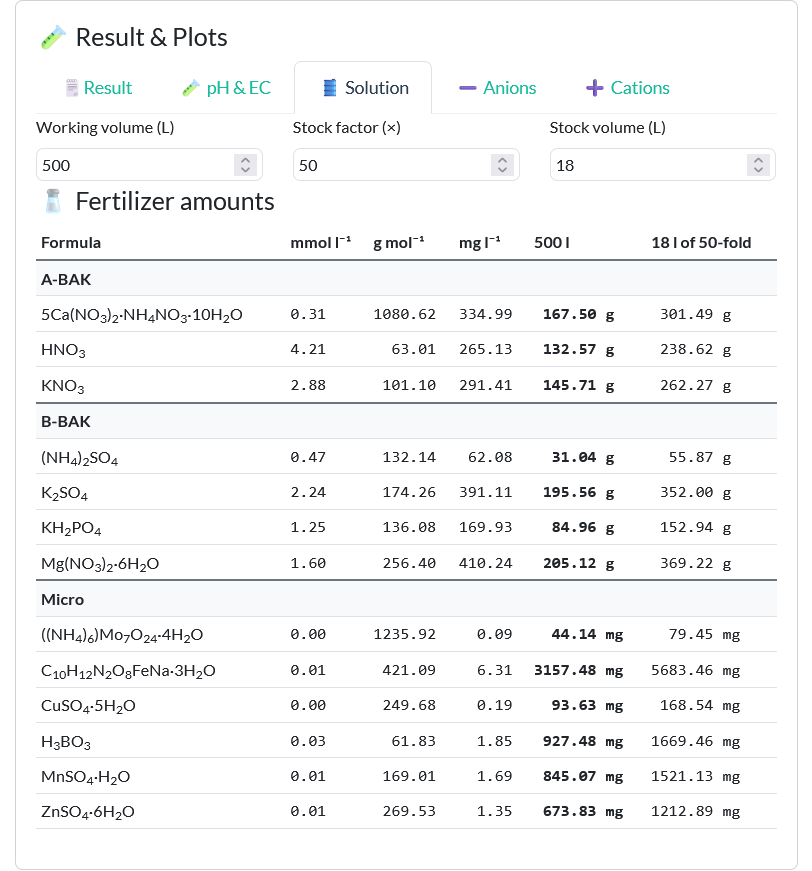
\includegraphics[width=15cm,height=\textheight,keepaspectratio]{Thesis_screenshots/tomato2final.png}

}

\caption{\label{fig-tomato-salt-composition}Fertilizer composition
calculated in the NutriCalc Shiny app for a tomato nutrient solution in
rockwool using tap water from Berlin postal code 14195. The formulation
is separated into A-BAK, B-BAK and micronutrient stock solution
fractions. Fertilizer requirements are given for the preparation of 500
L nutrient solution and for 18 L of 50-fold concentrated stock
solution.}

\end{figure}%

\subsubsection{Deviations from target}\label{deviations-from-target-1}

The tomato recipe specifies a target composition without Na, Cl, or Si.
In the calculated solution, these elements were present due to their
contribution from the tap water. Although the target composition was
matched with an SSRE of 0, absolute deviations remained for Na, Cl and
Si, resulting in an SSE of 7.69. The absolute errors were 2.03 mmol L⁻¹
for Na, 1.86 mmol L⁻¹ for Cl and 0.30 mmol L⁻¹ for Si. Of the Na
concentration, 0.015 mmol L⁻¹ originated from Fe-EDTA.

\subsubsection{pH and EC}\label{ph-and-ec-1}

The tap water from postal code 14195 had a calculated pH of 7.44 and an
EC of 0.86 mS cm⁻¹. Besides the ions considered in the target nutrient
composition, it supplied 2.02 mmol L⁻¹ Na⁺ and 1.86 mmol L⁻¹ Cl⁻,
contributing 0.09 and 0.13 mS cm⁻¹, respectively, to the total EC. The
electroneutral 0.3 mmol L⁻¹ Si present in the tap water did not
contribute to the overall EC.

The calculated final nutrient solution had a pH of 5.82. Ionic strength
amounted to 34.84 mmol L⁻¹, while the total concentration of charge
equivalents was 24.61 meq L⁻¹. The calculated EC was 2.81 mS cm⁻¹ and
the osmotic potential was −101.02 kPa. In the final solution, the
largest ionic contribution to EC was from NO₃⁻ at 0.89 mS cm⁻¹, followed
by K⁺ at 0.58 mS cm⁻¹ and SO₄²⁻ at 0.45 mS cm⁻¹

\subsection{Case study III --- Research scientist: nutrient formulation
for a novel halophyte (Salicornia) using mixed water
sources}\label{case-study-iii-research-scientist-nutrient-formulation-for-a-novel-halophyte-salicornia-using-mixed-water-sources}

\subsubsection{Achieved composition}\label{achieved-composition-2}

The calculated mixed water consists of 90 \% tap water from Berlin
postal code 10997 and 10 \% demineralised water, thereby reducing the
chloride concentration of the water source to 1.5 mmol L⁻¹. Based on
this water composition and the reference recipe ``Propagation vegetable
plants in rockwool'' reported by Sonneveld \& Straver (1994), chloride
is set to 1.5 mmol L⁻¹, yielding a calculated sodium concentration of
5.5 mmol L⁻¹ to maintain electroneutrality. Since ammonium nitrate
(NH₄NO₃) is excluded from the permissible fertilizer set, the target
composition is achieved using an alternative fertilizer combination. The
final fertilizer amounts are expressed for the preparation of 5 L stock
solution.

\subsubsection{Deviations from target}\label{deviations-from-target-2}

Only negligible deviations from the target composition were observed in
the achieved solution (SSE = 0.07; SSRE = 0). The calculated solution
contained 5.5 mmol L⁻¹ Na and 1.5 mmol L⁻¹ Cl, consistent with the
target composition and the mixed water source. The only remaining
absolute deviation concerned Si contributed by the tap water, which was
not specified as a target and therefore caused a small SSE.

\begin{figure}[H]

{\centering 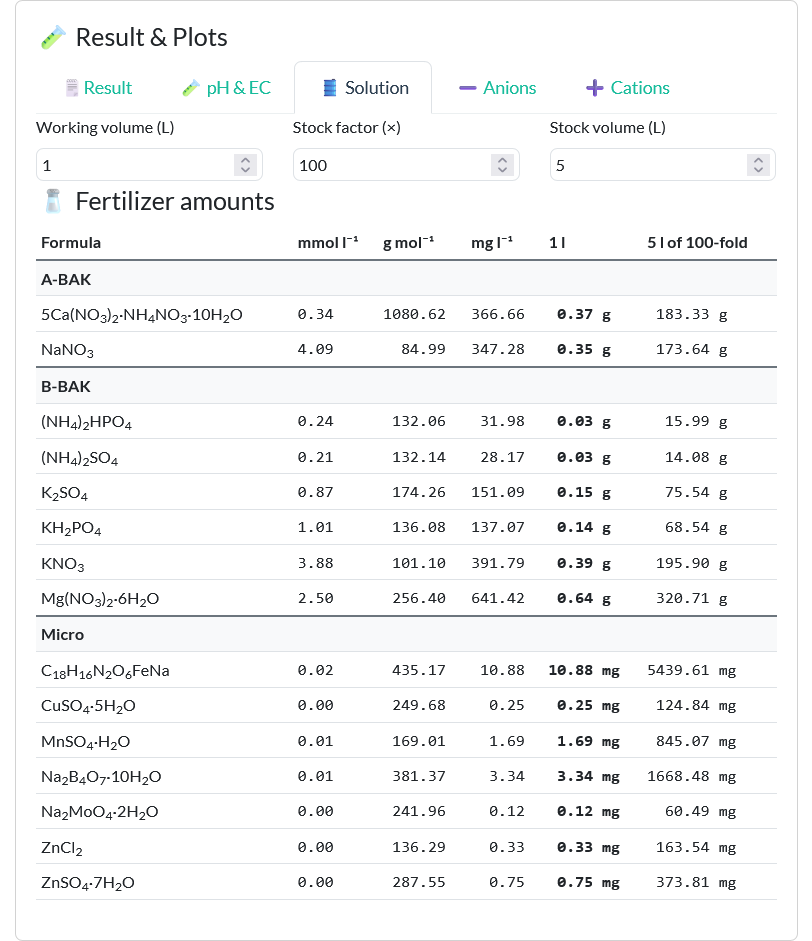
\includegraphics[width=15cm,height=\textheight,keepaspectratio]{Thesis_screenshots/case3_salts.png}

}

\caption{Screenshot of the fertilizer composition calculated in the
NutriCalc Shiny app for a halophyte nutrient solution prepared from a
mixture of tap water from Berlin postal code 10997 and deionized water.
The formulation is shown separately for A-BAK, B-BAK and the
micronutrient stock solution. Fertilizer requirements are reported for
the preparation of 5 L of 100-fold concentrated stock solution.}

\end{figure}%

\subsubsection{pH and EC}\label{ph-and-ec-2}

The calculated final nutrient solution had a pH of 7.19. Ionic strength
amounted to 39.47 mmol L⁻¹, while the total concentration of charge
equivalents was 28.60 meq L⁻¹. The calculated EC was 3.09 mS cm⁻¹ and
the osmotic potential was −111.29 kPa. The largest ionic contributions
to EC were from NO₃⁻ (1.07 mS cm⁻¹), K⁺ (0.45 mS cm⁻¹) and Ca²⁺ (0.39 mS
cm⁻¹). In addition, Na⁺ and Cl⁻ contributed 0.25 and 0.10 mS cm⁻¹,
respectively.

\chapter{Discussion}\label{discussion}

\section{Solver robustness and formulation
performance}\label{solver-robustness-and-formulation-performance}

Across the evaluated formulations, the solver reproduced most published
target compositions exactly or with only very small residual deviations.
This indicates that the implemented fertilizer matrix is sufficiently
expressive for a broad range of horticultural nutrient solutions. In
particular, the crop specific targets from Sonneveld \& Straver (1994)
were matched with SSE and SSRE values close to zero in most cases,
showing that the combination of stoichiometric matrix construction and
normalised NNLS optimisation is capable of representing many practically
relevant formulation problems with high fidelity.

Where deviations remained, they were chemically interpretable rather
than arbitrary numerical failures. This is important because it means
that residual error in the present framework should not immediately be
interpreted as an algorithmic weakness. Instead, it often reflects
specific properties of the fertilizer representation or of the target
vector itself.

Salts used in the solver were selected on the basis of their solubility
and their reported use in hydroponics. Salts that are not water soluble
but may still be relevant in soil based systems were therefore not
included in the implemented salt matrix.

The small SSE values reported for the crop set of Sonneveld \& Straver
(1994) are mainly caused by the use of chelated Fe sources in the salt
matrix. In the implemented representation, Fe chelates introduce Na as a
counter ion. Accordingly, a non zero Na contribution can occur in the
achieved solution even when Na is absent from the published target
vector. This should not be interpreted as a substantive mismatch in the
nutritionally relevant targets, but rather as a consequence of using
chemically realistic Fe fertilizers. Consistent with this
interpretation, SSE drops to zero when the Na target is set equal to the
Fe associated Na contribution.

A second recurring case involves recipes containing Si, commonly at
around 0.75 mmol L⁻¹. In the present matrix, Si is supplied via
K\textsubscript{2}SiO\textsubscript{3}, which necessarily introduces
additional K and also behaves as a strongly basic reagent. Consequently,
exact matching depends on whether this coupled K contribution is
represented in the target vector and or corrected by acid addition. When
Si is omitted, or when the corresponding K contribution is accounted for
explicitly, SSRE approaches zero.

This indicates that the residual mismatch in Si containing recipes is
not primarily caused by numerical instability of the optimiser, but by
chemically coupled fertilizer behaviour. In other words, the difficulty
lies less in the NNLS procedure itself than in the fact that silicon
supply through potassium silicate cannot be treated independently of its
accompanying alkalinity and counter ion contribution, because it behaves
effectively as a base used in the role of a salt.

Although Si is generally considered a beneficial rather than an
essential element, positive effects on yield and disease suppression
have been reported (Rengel et al., 2023; Voogt \& Sonneveld, 2001).
Practical use of potassium silicate often requires stoichiometric acid
compensation. In the formulations discussed by Voogt \& Sonneveld
(2001), this was addressed by combining silicate addition with nitric
acid and with corresponding adjustment of nitrate salts.

The fact that Si containing cases improved when acid and base correction
was allowed in NutriCalc therefore supports rather than undermines the
chemical plausibility of the framework. Taken together, the results
suggest that NutriCalc performs robustly within the tested horticultural
domain and that the remaining deviations can usually be traced back to
identifiable chemical causes.

The three case studies illustrate distinct formulation constraints. The
Hoagland case showed that exact reconstruction remained possible even
when the original calcium nitrate source was unavailable and replaced by
calcium ammonium nitrate. The tomato case demonstrated the effect of
source-water correction, where Na, Cl and Si from Berlin-Dahlem tap
water remained present in the final solution. The halophyte case
extended the workflow to mixed-water formulation, where sodium and
chloride constraints were part of the experimental design. Together,
these examples show that NutriCalc can be applied not only to recipe
reconstruction, but also to constrained formulation scenarios involving
fertilizer substitution, source-water chemistry and experimental
manipulation of specific ions.

\section{Exact solvability, electroneutrality and non
uniqueness}\label{exact-solvability-electroneutrality-and-non-uniqueness}

In this context, an electroneutral target is defined as a target vector
for which the sum of cation and anion charge equivalents is balanced. A
non electroneutral target is a target vector for which this condition is
not fulfilled. Electroneutrality is a necessary but not sufficient
condition for exact solvability when only electrically neutral salts are
considered. Exact solvability also depends on the selected fertilizer
set.

If the target is electroneutral and the available fertilizers span the
required composition, the solver may find an exact solution. In such
cases, both SSE and SSRE are zero, indicating that all targets have been
matched exactly in both absolute and relative terms. However, this does
not imply that the solution is unique. Different fertilizer combinations
may produce the same final nutrient composition (Steiner, 1961). Some
alternative solutions differ only in the hydration state of a salt, for
example Ca(NO\textsubscript{3})\textsubscript{2} versus
Ca(NO\textsubscript{3})\textsubscript{2}·4H\textsubscript{2}O, whereas
others may involve chemically distinct fertilizer combinations. In some
cases, the number of exact solutions may be effectively infinite because
different salts can compensate for one another while preserving the same
final nutrient profile.

Accordingly, the NNLS solver returns one admissible non negative
optimum, but it does not characterise the full set of possible exact
solutions. Users can nevertheless influence the returned solution by
restricting the fertilizer set through the selection and deselection of
salts. In addition, small fertilizer amounts may appear in the solution
if they provide even a minor reduction in the objective function. Thus,
an exact or near exact solution is not necessarily the chemically
simplest or most practical one.

If the target is non electroneutral, it cannot be matched exactly using
only electrically neutral salts. In that case, the solver returns the
non negative best fit solution that minimises the residual error.
Because NutriCalc normalises residuals by target magnitude, the
optimisation criterion primarily minimises the sum of squared relative
errors for non zero targets and the sum of squared absolute errors for
zero targets.

A useful implication of this formulation is that infeasible targets are
not solved in an intuitively arithmetic sense, but according to the
relative structure of the objective function. When a target cannot be
matched exactly, the remaining mismatch is distributed according to the
row scaling and the imposed weights. Thus, residual error should not be
interpreted simply as failure. It may instead indicate that the target
is not electroneutral, that the selected fertilizer set does not span
the target composition, or that chemically realistic fertilizer sources
introduce unavoidable side contributions.

\section{Error metrics and interpretation of residual
deviation}\label{error-metrics-and-interpretation-of-residual-deviation}

Reported errors quantify the deviation between target and achieved
nutrient concentrations. For each nutrient, the formulation output
reports the absolute error and, when the target is non zero, the
relative error. Two aggregate metrics are derived: the sum of squared
errors, SSE and the sum of squared relative errors, SSRE. The per
nutrient errors indicate which nutrients deviate from the target, by how
much and in which direction. The squared error metrics summarise overall
solution quality.

The optimisation itself is based on a row normalised non negative least
squares, NNLS, formulation. Residuals are scaled by a nutrient specific
factor: for nutrients with non zero targets, deviations are normalised
by the corresponding target concentration. For nutrients with zero
targets, a scaling factor of one is applied. As a result, all nutrients,
including those with targets set to zero, are actively included in the
objective function. Any non zero achieved concentration for a zero
target nutrient contributes a quadratic penalty and is therefore
discouraged during optimisation.

SSE reflects the total squared deviation across all nutrients and
therefore captures leakage into zero target nutrients. SSRE, in
contrast, summarises squared relative deviations only for nutrients with
non zero targets and serves as the primary performance indicator for how
closely specified targets were matched. However, both SSE and SSRE are
post hoc reporting metrics. The solver decision is determined by the
normalised and weighted NNLS objective. Consequently, a formulation with
slightly lower relative deviation for non zero targets may still be
rejected if it introduces substantial unintended supply of zero target
nutrients, because this increases the overall objective value.

Without normalisation, an objective based solely on squared absolute
errors would bias the optimisation toward macronutrients, since
deviations in the µmol L\textsuperscript{-1} range would be numerically
negligible compared with deviations in the mmol L\textsuperscript{-1}
range. Row wise normalisation therefore ensures that proportional
deviations are penalised on a comparable scale, preventing magnitude
driven bias and enabling balanced optimisation for both macro and
micronutrients.

In this sense, SSE and SSRE should not be interpreted as direct
optimisation targets, but as complementary descriptors of the achieved
solution. SSE is particularly informative for identifying chemically
relevant leakage into nutrients that were intended to remain absent,
whereas SSRE is more informative for evaluating proportional agreement
with specified non zero targets.

A useful illustration is the 1:1 salt coupling case, for example NaCl or
NH\textsubscript{4}NO\textsubscript{3}. If the targets are 1 mmol
L\textsuperscript{-1} for one ion and 2 mmol L\textsuperscript{-1} for
the coupled counter ion, relative error minimisation yields an optimum
at 1.2 mmol L\textsuperscript{-1} rather than the arithmetic midpoint of
1.5 mmol L\textsuperscript{-1}. This demonstrates a non intuitive but
important property of the normalised objective: the optimum is shifted
toward the smaller target because deviations are scaled relative to
target magnitude.

\section{Weighting and two stage optimisation as practical control
tools}\label{weighting-and-two-stage-optimisation-as-practical-control-tools}

Weighting is optional, so the solver can also be used in an unweighted
form, in which all nutrients contribute equally after normalisation. If
weights are applied, the problem becomes a weighted non negative least
squares problem, in which deviations in highly weighted nutrients
contribute more strongly to the objective function than deviations in
nutrients with lower weights. Lowering the weight of one nutrient shifts
more of the residual error to that nutrient and allows the remaining
nutrients to be matched more closely. In practical terms, this means
that one nutrient can be deliberately sacrificed to improve the overall
fit of the others when the target profile is difficult or impossible to
achieve with the selected salts.

This feature is particularly useful for chemically constrained
formulations. If one nutrient cannot be matched simultaneously with all
others because of stoichiometric coupling within the available
fertilizers, reducing its weight may substantially improve the fit for
the remaining targets. When the second solver stage is enabled,
additional adjustment with acids or bases may further improve the final
composition and partially compensate for such trade offs.

It was possible to achieve an exact match between target and achieved
nutrient concentrations for most of the crop set of Sonneveld \& Straver
(1994) using the one stage salts only solver. This demonstrates that the
implemented salt matrix is sufficiently comprehensive to represent many
standard horticultural target profiles.

The two stage solver nevertheless provides an important extension when
an exact solution is not achievable with neutral salts alone. In this
architecture, the first stage fits the composition using neutral
fertilizer salts, whereas acids and bases are introduced only in a
second corrective step. This separation is chemically meaningful because
it prevents acids and bases from acting as unrestricted first stage
degrees of freedom that could improve the numerical fit while reducing
interpretability of the resulting fertilizer composition.

The results support this design particularly for pH active or
stoichiometrically awkward cases, such as silicate containing
formulations. The two stage framework should therefore not be understood
merely as a numerical convenience, but as a practically motivated
control mechanism that balances solvability, chemical interpretability
and operational realism.

\section{Electroneutrality and pH as coupled
constraints}\label{electroneutrality-and-ph-as-coupled-constraints}

Electroneutrality is one of the most fundamental principles in nutrient
solution formulation. In any aqueous electrolyte solution, the sum of
positive charges must equal the sum of negative charges. Thus, the total
charge contributed by cations is balanced by the total charge
contributed by anions (Kalka, 2024). While many dissolved compounds
dissociate into well defined cations and anions and therefore contribute
predictably to charge balance, some nutrients exist in different ionic
species depending on pH. At the same time, pH should not be understood
merely as a measure of hydrogen ion concentration, but more accurately
as a measure of hydrogen ion activity. From this perspective, pH can be
interpreted as a dependent variable constrained by the electroneutrality
condition in aqueous solution (Stumm \& Morgan, 1996). Accordingly, the
activities of H\textsubscript{3}O\textsuperscript{+} and
OH\textsuperscript{-} adjust in conjunction with pH dependent speciation
systems such as phosphate, sulfate, carbonate, borate and silicate to
maintain charge balance, rather than being determined solely by the
stoichiometric addition and neutralisation of acid and base.

Electroneutrality ultimately determines whether a target nutrient
composition is physically realisable. In the optimisation procedure, non
negativity of salt addition was implemented explicitly as a mathematical
constraint, whereas electroneutrality was not imposed as an additional
constraint. This is because fertilizer salts contribute ions in
stoichiometrically balanced combinations. Acid or base addition changes
pH and ionic speciation without violating the overall charge balance of
the solution. Consequently, if a target nutrient profile is itself not
electroneutral, no exact solution exists and the solver can only
minimise the deviation from the specified targets.

This is directly relevant for interpretation of pH within the framework.
pH should not be treated as an independently selectable scalar, but as
an emergent property of charge balance, acid base equilibria and
activities. Integrating charge balance based pH estimation therefore
extends formulation from simple nutrient matching toward chemically
coherent solution evaluation.

\section{Role of pH and EC modelling in the
workflow}\label{role-of-ph-and-ec-modelling-in-the-workflow}

A notable strength of the framework is that formulation is not treated
as complete once nutrient targets have been matched. Estimated pH and EC
provide a second interpretive layer linking nutrient composition to
broader physicochemical behaviour. This is relevant because two
solutions with similar nominal nutrient targets can differ in buffering,
ionic strength, conductivity or pH response depending on fertilizer
selection, water composition and corrective additions.

The pH of a nutrient solution is a critical parameter that determines
the speciation of elements across their various physicochemical forms
(free ions, complexes, chelates, ion pairs, solid and gaseous phases and
different oxidation levels) and is therefore critical for nutrient
bioavailability (Rijck \& Schrevens (1998)). The implemented pH
estimation module provides a practical way to evaluate the expected pH
of the formulated solution based on its composition and the applied acid
or base correction. This allows users to anticipate whether the
resulting pH will be within a desirable range for plant growth and to
make informed decisions about formulation adjustments if necessary.

While both γ activity correction models (Davies and Debye--Hückel) were
evaluated, using the phosphate buffer system for pH prediction and KCl
conductivity solutions at 25 °C for EC prediction, the Davies model
showed closer agreement with the reference values in both cases. It was
therefore selected as the default activity correction for pH and EC
prediction in NutriCalc.

Within the tested ranges, the implemented pH and EC models provided
useful chemically informed approximations. The Davies activity
correction showed better pH agreement than the limiting Debye-Hückel
model in phosphate buffer comparisons. Likewise, EC estimation based on
diffusion coefficients together with Davies activity correction agreed
closely with reference KCl values and with PHREEQC based comparisons,
whereas simpler empirical approaches tended to underestimate
conductivity at higher concentrations.

These modules do not replace full geochemical simulation. Their value
lies in practical workflow integration because users can evaluate not
only whether a target vector can be approximated, but also what pH and
EC consequences follow from the achieved formulation.

\section{Relevance of the mass balance
approach}\label{relevance-of-the-mass-balance-approach}

``Judging from their publications and statements, it would seem that
many investigators have grown crops in a solution chosen largely at
random and that, where the results have been successful, they have
recommended that solution as being specific for the particular crop
concerned.'' (Steiner, 1961)

Optimal nutrient solutions can be formulated using the principle of mass
balance (Langenfeld et al., 2022). Bugbee et al. (Bugbee \& Noah James
Langenfeld, 2024) reported a related set of mass balance based nutrient
recipes for monocots, dicots and \emph{Cannabis}. In contrast to
empirically derived nutrient recipes, this approach seeks to relate
nutrient supply directly to plant demand. Plant nutrient demand can be
approximated from tissue nutrient composition in combination with plant
water consumption, thereby linking absolute nutrient uptake to water
uptake. Langenfeld et al. (2022) distinguish between active uptake (N,
P, K, Mn), intermediate uptake (Mg, S, Fe, Cu, Zn, Mo, Ni, Cl) and
passive uptake (Ca, B). Passively taken up nutrients such as Ca are
closely related to transpired water and are therefore well suited to a
mass balance approach. Since tissue analysis represents a destructive
end point measurement, non linearities in active nutrient uptake
kinetics, including transitions between high affinity and low affinity
transport systems, are of limited relevance in this context. With both
WUE and tissue analysis, the exact temporal dynamics of uptake do not
need to be resolved explicitly, as the temporal dimension is subsumed
into the final nutrient solution composition. Thus, although active and
passive uptake differ mechanistically and kinetically, these differences
converge in the relationship between cumulative water use and the plant
tissue nutrient content observed at harvest.

On this basis, crop specific target concentrations for the nutrient
solution can be derived. Under ideal conditions, such a formulation
would maintain the residual or recirculating solution in approximate
balance over time, thereby minimising the accumulation or depletion of
individual nutrients.

The present framework is particularly relevant here because a
biologically plausible demand vector is not automatically a chemically
realisable nutrient solution. Even if tissue composition and water use
define a meaningful elemental target, this still has to be translated
into an ionic target and then into a feasible fertilizer composition.
NutriCalc provides a transparent way to make this translation explicit.

A remaining limitation of tissue based mass balance approaches is the
translation of total plant N into a chemically feasible nutrient
solution target. Specifically, total N must be partitioned into nitrate
and ammonium. To address this, the present work introduces a refinement
of the mass balance approach in which total N is partitioned into
NO\textsubscript{3}--N and NH\textsubscript{4}--N by imposing
electroneutrality as an explicit formulation constraint. This step
enables the derivation of nutrient solutions that are chemically
plausible and electrochemically balanced. In the example considered
here, based on Langenfeld et al. (2022), a total N concentration of 90
mg L\textsuperscript{-1} yields a partitioning of 82 mg
L\textsuperscript{-1} NO\textsubscript{3}--N and 8 mg
L\textsuperscript{-1} NH\textsubscript{4}--N.

This does not yet constitute a full physiological model of nutrient
uptake, but it is a meaningful methodological step. It bridges
biological demand estimation and chemically constrained fertilizer
realisation within one transparent computational framework.

\section{Comparison with existing formulation
approaches}\label{comparison-with-existing-formulation-approaches}

Existing nutrient formulation practice spans fixed recipes, manual
iterative balancing, spreadsheet tools and dedicated software. Classical
approaches such as the universal algorithm of Sonneveld et al. (1999)
are chemically informed and practically valuable, but they are not
necessarily expressed as explicit constrained optimisation frameworks.
Spreadsheet based calculators can be useful in practice, but often
remain difficult to extend reproducibly and may obscure the underlying
calculation logic. Other software such as HydroBuddy offers flexible
nutrient formulation functionality, but NutriCalc contributes a distinct
combination of explicit stoichiometric representation, weighted row
normalised NNLS fitting, charge balance oriented evaluation and modular
open source implementation in R.

The main contribution of NutriCalc is therefore not merely that it
calculates fertilizer quantities, but that it formalises nutrient
formulation as a transparent, reproducible and modifiable constrained
optimisation problem. The R implementation supports programmable
workflows and integration with other analyses, whereas the Shiny
interface broadens accessibility for users without programming
experience.

\section{Limitations and scope}\label{limitations-and-scope}

Despite its strengths, the framework has clear limitations. First,
precipitation reactions are not modeled beyond BAK separation. A target
may therefore appear feasible in dissolved ion terms while being
unstable in concentrated stock solutions.

Second, chemical speciation remains simplified. Major acid base systems
and fixed charge chelates are represented, but a full complexation model
is not implemented yet.

Third, the activity corrections used for pH and EC estimation remain
approximate. Debye Hückel and Davies models are suitable for dilute to
moderately concentrated systems, but they do not capture all non ideal
effects at higher ionic strengths.

Fourth, non zero residuals may reflect limitations of the selected
fertilizer matrix rather than universal chemical impossibility. Exact
solvability is always conditional on the implemented fertilizer set,
which is not yet complete.

Fifth, the optimisation currently targets nutrient fit rather than
explicit minimisation of cost, number of salts or operational
complexity. Although users can partly influence the returned solution
through salt selection and weighting, these objectives are not yet
formalised directly.

Finally, the framework is a formulation and evaluation model rather than
a crop growth model. It can represent and assess nutrient solution
chemistry, but it does not predict plant response, uptake kinetics or
recirculating system dynamics over time.

These limitations define the scope of the framework rather than
invalidating its usefulness. NutriCalc should therefore be understood as
a transparent and extensible formulation tool that captures major
stoichiometric and physicochemical constraints, while leaving more
advanced geochemical and biological dynamics to future development.

\chapter{Conclusions and Outlook}\label{conclusions-and-outlook}

\section{Scientific contribution}\label{scientific-contribution}

This thesis developed \texttt{NutriCalc}, an open-source computational R
package with a Shiny interface for the formulation, analysis and
optimisation of nutrient solutions in horticulture. The work formalised
nutrient-solution design as a constrained linear optimisation problem
and implemented this formulation using non-negative least squares. In
doing so, it linked stoichiometric conversion, target-based
optimisation, water-source correction and chemically informed evaluation
of pH and electrical conductivity within one transparent workflow.

The results showed that a broad range of published horticultural target
solutions can be reproduced exactly or with only minor residual
deviations. Where deviations remained, these were generally chemically
interpretable and could often be traced to fertilizer representation,
electroneutrality constraints or chemically coupled sources such as
potassium silicate. Beyond reproducing established recipes, the
framework also demonstrated how nutrient formulation can be extended
toward mass-balance-derived targets and charge-balance-based
interpretation.

Taken together, the thesis shows that nutrient-solution formulation can
be moved from recipe-based and partly opaque practice toward a
reproducible, optimisation-based and chemically explicit computational
workflow.

\section{Practical relevance for
horticulture}\label{practical-relevance-for-horticulture}

The practical relevance of the framework lies in its applicability to
both research and horticultural practice. For researchers, NutriCalc
provides a transparent tool for constructing and comparing nutrient
treatments under explicitly defined chemical constraints. For
practitioners, it offers a flexible way to formulate crop-specific
nutrient solutions while accounting for local water quality, available
fertilizers and physicochemical properties of the final solution.

By combining an R package with a Shiny-based graphical user interface,
the framework is accessible both for programmable analytical workflows
and for users without coding experience. In this sense, NutriCalc
contributes not only methodologically but also operationally to digital
nutrient management in horticulture.

\section{Limitations}\label{limitations}

The scope of the present thesis is limited in several respects.
Precipitation reactions and full complexation were not modeled
explicitly, so the framework should not be interpreted as a complete
geochemical simulation environment. Likewise, the pH and EC calculations
remain approximations based on selected equilibrium and activity models.
The pH and EC evaluations should therefore be understood as calibration
checks rather than comprehensive empirical validation. pH validation was
limited to a phosphate buffer system, while EC validation was limited to
KCl standards. Neither test replaces validation across chemically
diverse horticultural nutrient solutions. In addition, exact solvability
always depends on the implemented fertilizer matrix, which is
necessarily incomplete. The present fertilizer set was selected based on
solubility and reported use in hydroponics, but it does not yet include
all possible fertilizers or micronutrients.

The framework is therefore best understood as a transparent formulation
and evaluation tool that captures major stoichiometric and
physicochemical constraints, but not the full complexity of nutrient
chemistry or crop response.

\section{Future extensions}\label{future-extensions}

Future development of NutriCalc could expand both the scientific scope
of the framework and its practical applicability in horticultural
research and nutrient-solution management. One important direction is
the expansion of the fertilizer database. This includes adding further
compounds commonly used in horticultural practice, enabling users to
define custom salts directly within the application and extending the
system with additional micronutrients such as Ni and Co together with
appropriate fertilizer sources. Such developments would increase
flexibility and allow the software to be adapted to different regional
fertilizers and cultivation systems.

A second direction concerns the chemical model. In addition to the
current treatment of nutrient composition, pH and EC, future versions
could incorporate more detailed chemical speciation and explicit
precipitation modelling. This would improve applicability particularly
for the formulation of concentrated stock solutions and would further
strengthen the chemical realism of the framework.

A third direction concerns the optimisation framework itself. At
present, formulation is based on an NNLS approach that focuses on
matching target nutrient concentrations as closely as possible. Future
versions could include additional constraints such as fertilizer price,
thereby allowing the formulation process to reflect not only chemical
targets but also economic considerations.

A fourth direction involves the representation of nutrient targets and
the expansion of built-in datasets. Because the internal formulation
matrix operates on a stoichiometric basis, conversion between molar and
mass-based units is straightforward. NutriCalc could therefore be
extended to accept target nutrient profiles not only in mmol L⁻¹ but
also in mass-based units or nutrient percentages, which would improve
usability for users more familiar with commercial fertilizer labels and
analytical results reported in such forms. Likewise, the dataset of
target nutrient profiles could be expanded to include a wider range of
crops, production systems and developmental stages. For example,
stage-specific target profiles could be provided for crops such as
tomato, in which nutrient demand changes substantially between
vegetative growth, flowering and fruit development. A simple external
input format such as CSV could facilitate maintenance and extension of
such datasets and would also allow users to adapt recipes to their own
conditions.

A fifth direction is the further development of reporting and user
interaction. From a practical perspective, a particularly useful next
step would be the integration of export functions into the Shiny
application. Because this thesis was developed in Quarto, PDF and CSV
exports could be implemented to generate structured reports for
individual nutrient formulations. These reports could include the
selected fertilizer salts, achieved nutrient concentrations, deviations
from target values and predicted pH and EC together with supporting
tables and visualisations. This would strengthen the value of NutriCalc
as both a scientific and an applied tool.

Overall, future extensions of NutriCalc could strengthen the package in
three broad areas: broader input flexibility, more advanced chemical and
optimisation routines and improved reporting and user interaction. The
most important future extension, however, is the integration of
experimental data, particularly for the mass-balance approach, in order
to derive more precisely balanced and crop-specific nutrient recipes for
closed hydroponic systems.

\chapter{Summary}\label{summary}

This thesis addresses nutrient-solution formulation in horticulture,
particularly in hydroponic and other soilless systems, where solution
composition must be defined precisely under chemical and practical
constraints. In practice, nutrient recipes are often derived from fixed
formulations or manual trial-and-error adjustment. Such approaches are
difficult to reproduce consistently across studies and prone to
conversion errors, especially when water quality, fertilizer composition
and different unit systems must be considered simultaneously.

To address this problem, the thesis developed \texttt{NutriCalc}, an
open-source computational framework in R for the formulation, evaluation
and optimisation of nutrient solutions. The central methodological
contribution was the development of a reproducible computational
pipeline that replaces ad hoc recipe formulation with mathematical
optimisation. Nutrient-solution design was formalised as a constrained
linear optimisation problem and solved using non-negative least squares,
allowing fertilizer combinations to be calculated transparently while
ensuring physically meaningful, non-negative quantities.

The framework integrated stoichiometric conversion of fertilizer
compounds, mapping to canonical nutrient targets, transformation between
molar and mass-based units and correction for ions already present in
the source water. In this way, NutriCalc established a consistent
workflow linking fertilizer compounds, nutrient targets and practical
concentration units. Beyond nutrient matching, it also incorporated
chemically informed evaluation of electroneutrality, pH and electrical
conductivity, connecting optimisation results to physicochemical
properties relevant for experimental interpretation and practical
nutrient management. A further contribution of the thesis was the
implementation of the framework in two complementary forms: a
programmable R package and a Shiny-based graphical user interface. This
dual design supports both reproducible analytical workflows in research
and interactive use in horticultural practice.

The results showed that a broad range of published horticultural target
solutions could be reconstructed exactly or with only small residual
deviations. Where exact fits were not possible, these deviations were
generally chemically interpretable and could often be traced to
identifiable constraints such as limited fertilizer choice,
stoichiometric ion coupling across salts or electroneutrality
requirements. The case studies further demonstrated that the framework
can be applied to more complex scenarios involving alternative
fertilizer availability, local water composition and mixed water
sources.

Overall, the thesis showed that nutrient-solution design can be shifted
from a recipe-based and partly opaque practice to a reproducible,
optimisation-based and chemically explicit workflow, providing both a
methodological framework for horticultural research and a practical
basis for transparent nutrient management in soilless cultivation
systems.

\chapter{References}\label{references}

\phantomsection\label{refs}
\begin{CSLReferences}{1}{0}
\bibitem[\citeproctext]{ref-Amelung.2018}
Amelung, W., Blume, H.-P., Fleige, H., Horn, R., Kandeler, E.,
Kögel-Knabner, I., Kretzschmar, R., Stahr, K., Wilke, B.-M., Scheffer,
F., \& Schachtschabel, P. (2018). \emph{{Scheffer/Schachtschabel
Lehrbuch der Bodenkunde}} (17., {ü}berarbeitete und erg{ä}nzte Auflage).
Berlin; Heidelberg: {Springer Spektrum}.
\url{https://doi.org/10.1007/978-3-662-55871-3}

\bibitem[\citeproctext]{ref-Appelo.2005}
Appelo, C. A. J. (2005). \emph{{Geochemistry, groundwater and
pollution}} (Second edition). Leiden: {A.A. Balkema Publishers}.
\url{https://doi.org/10.1201/9781439833544}

\bibitem[\citeproctext]{ref-Appelo.2010}
Appelo, C. A. J. (2010). \emph{{SPECIFIC CONDUCTANCE: how to calculate,
to use, and the pitfalls}}. Retrieved from
\url{https://www.hydrochemistry.eu/exmpls/sc.html}

\bibitem[\citeproctext]{ref-BIPM.2019}
BIPM. (2019). \emph{{The International System of Units (SI)}}. {Bureau
International des Poids et Mesures}.
\url{https://doi.org/10.59161/AUEZ1291}

\bibitem[\citeproctext]{ref-Bower.1955}
Bower, V. E., \& Bates, R. G. (1955). {pH values of the Clark and Lubs
buffer solutions at 25 C}. \emph{{Journal of Research of the National
Bureau of Standards}}, \emph{55}, 197. Retrieved from
\url{https://api.semanticscholar.org/CorpusID:101259939}

\bibitem[\citeproctext]{ref-Bugbee.2024}
Bugbee, B., \& Noah James Langenfeld. (2024). \emph{{Utah hydroponic
solutions}}. {Utah State University}. Retrieved from
\url{https://digitalcommons.usu.edu/cpl_nutrients/2/}

\bibitem[\citeproctext]{ref-BWB.2026}
BWB. (2026). \emph{{Analysedaten nach Postleitzahlen: Bitte geben Sie
Ihre Postleitzahl in das Suchfenster ein, um die Werte f{ü}r Ihren
Wohnbezirk zu erhalten:}} Retrieved from
\url{https://www.bwb.de/de/analysedaten-nach-postleitzahlen.php?PLZ=x}

\bibitem[\citeproctext]{ref-Chang.2025}
Chang, W., Cheng, J., Allaire, J. J., Sievert, C., Schloerke, B., Xie,
Y., Allen, J., McPherson, J., Dipert, A., \& Borges, B. (2025).
\emph{{shiny: Web Application Framework for R}}. {Comprehensive R
Archive Network (CRAN)}.
\url{https://doi.org/10.32614/CRAN.package.shiny}

\bibitem[\citeproctext]{ref-FernandezPinto.2022}
Fernández Pinto, D. (2022). \emph{{HydroBuddy: An open source nutrient
calculator for hydroponics and general agriculture}}. Retrieved from
\url{https://github.com/danielfppps/hydrobuddy}

\bibitem[\citeproctext]{ref-George.2012}
George, E., Horst, W. J., \& Neumann, E. (2012). {Adaptation of Plants
to Adverse Chemical Soil Conditions}. In \emph{{Marschner's Mineral
Nutrition of Higher Plants}} (pp. 409--472). Elsevier.
\url{https://doi.org/10.1016/b978-0-12-384905-2.00017-0}

\bibitem[\citeproctext]{ref-Haynes.2017}
Haynes, W. M. (Ed.). (2017). \emph{{CRC Handbook of chemistry and
physics}} (97th edition). Boca Raton; London; New York: {CRC Press}.

\bibitem[\citeproctext]{ref-Hewitt.1966}
Hewitt, E. J. (1966). \emph{{Sand and water culture methods used in the
study of plant nutrition}} (2. rev. edition). Farnham Royal:
{Commonwealth Agricultural Bureaux}.

\bibitem[\citeproctext]{ref-Hoagland.1920}
Hoagland, D. R. (1920). {Optimum Nutrient Solutions for Plants}.
\emph{{American Association for the Advancement of Science}}. Retrieved
from \url{https://www.science.org/doi/10.1126/science.52.1354.562}

\bibitem[\citeproctext]{ref-Hoagland.1938}
Hoagland, D. R., \& Arnon, D. I. (1938). \emph{{The Water-Culture Method
for Growing Plants without Soil}}.

\bibitem[\citeproctext]{ref-Incrocci.2007}
Incrocci, L. (2007). \emph{{Nutrient Solution Calculator: Retrieved from
the Internet Archive (Wayback Machine)}} (Dipartimento di Biologia delle
Piante Agrarie, University of Pisa, Ed.). Retrieved from
\url{https://web.archive.org/web/20240813175407/https://www.wur.nl/en/research-results/projects-and-programmes/euphoros/calculation-tools/nutrient-solution-calculator.htm}

\bibitem[\citeproctext]{ref-Incrocci.2020}
Incrocci, L., M., Giménez Moolhuyzen, M., \& Guzmán Palomino, J. M.
(2020). \emph{{Calculadora de Soluciones Nutritivas (SN)}}. Retrieved
from \url{https://repositorio.ual.es/handle/10835/7670?show=full}

\bibitem[\citeproctext]{ref-Jones.2014}
Jones, J. B. (2014). \emph{{Complete guide for growing plants
hydroponically}}. Boca Raton: {CRC Press}.

\bibitem[\citeproctext]{ref-Jones.2024}
Jones, J. J., Shaw, C., Chen, T., Staß, C. M., Ulrichs, C., Riewe, D.,
Kloas, W., \& Geilfus, C. (2024). {Plant nutritional value of
aquaculture water produced by feeding Nile tilapia ( Oreochromis
niloticus ) alternative protein diets: A lettuce and basil case study}.
\emph{{Plants, People, Planet}}, \emph{6}(2), 362--380.
\url{https://doi.org/10.1002/ppp3.10457}

\bibitem[\citeproctext]{ref-Kalka.2020}
Kalka, H. (2020). \emph{{Electrical Conductivity based on Diffusion
Coefficients}}. Retrieved from \url{https://www.aqion.de/site/77}

\bibitem[\citeproctext]{ref-Kalka.2023}
Kalka, H. (2023). \emph{{Aktivit{ä}tskoeffizient und
Aktivit{ä}tsmodelle}}. Retrieved from \url{https://www.aqion.de/site/41}

\bibitem[\citeproctext]{ref-Kalka.2024}
Kalka, H. (2024). \emph{{Charge-Balance Error (CBE)}}. Retrieved from
\url{https://www.aqion.de/site/92}

\bibitem[\citeproctext]{ref-Knop.1860}
Knop, W. (1860). {Ueber die Ern{ä}hrung der Pflanzen durch w{ä}ssrige
L{ö}sungen bei Ausschlu{ß} des Bodens}. \emph{{Die Landwirthschaftlichen
Versuchs-Stationen}}, (2).

\bibitem[\citeproctext]{ref-Langenfeld.2022}
Langenfeld, N. J., Pinto, D. F., Faust, J. E., Heins, R., \& Bugbee, B.
(2022). {Principles of Nutrient and Water Management for Indoor
Agriculture}. \emph{{Sustainability}}, \emph{14}(16), 10204.
\url{https://doi.org/10.3390/su141610204}

\bibitem[\citeproctext]{ref-Lawson.1974}
Lawson, C. L., \& Hanson, R. J. (1974). \emph{{Solving least squares
problems}}. Englewood Cliffs, NJ: Prentice-Hall.

\bibitem[\citeproctext]{ref-Lawson.1995}
Lawson, C. L., \& Hanson, R. J. (1995). \emph{{Solving least squares
problems}} ({[}10. Dr.{]}). Philadelphia: SIAM.

\bibitem[\citeproctext]{ref-McCleskey.2012}
McCleskey, R. B., Nordstrom, D. K., \& Ryan, J. N. (2012). {Comparison
of electrical conductivity calculation methods for natural waters}.
\emph{{Limnology and Oceanography: Methods}}, \emph{10}(11), 952--967.
\url{https://doi.org/10.4319/lom.2012.10.952}

\bibitem[\citeproctext]{ref-Mullen.2024}
Mullen, K. M., \& van Stokkum, I. H. M. (2024). \emph{{The Lawson-Hanson
Algorithm for Non-Negative Least Squares (NNLS): An R interface to the
Lawson-Hanson implementation of an algorithm for non-negative least
squares (NNLS). Also allows the combination of non-negative and
non-positive constraints.}} {Comprehensive R Archive Network (CRAN)}.
\url{https://doi.org/10.32614/CRAN.package.nnls}

\bibitem[\citeproctext]{ref-Pardossi.2011}
Pardossi, Carmassi G., Diara C., I. L., Maggini R., \& Massa D. (2011).
\emph{{Fertigation and substrate management in closed soilless
culture}}. {Dipartimento di Biologia delle Piante Agrarie, University of
Pisa}.

\bibitem[\citeproctext]{ref-Parkhurst.2013}
Parkhurst, D. L., \& Appelo, C. A. J. (2013). \emph{{Description of
input and examples for PHREEQC version 3: A computer program for
speciation, batch-reaction, one-dimensional transport, and inverse
geochemical calculations}}. Reston, Virginia: {U.S. Department of the
Interior U.S. Geological Survey}. Retrieved from
\url{http://purl.fdlp.gov/GPO/gpo37078}

\bibitem[\citeproctext]{ref-Positteam.2025}
Posit team. (2025). \emph{{RStudio: Integrated Development Environment
for R.}} Posit Software, PBC. Retrieved from \url{http://www.posit.co/}

\bibitem[\citeproctext]{ref-Pratt.2001}
Pratt, K. W., Koch, W. F., Wu, Y. C., \& Berezansky, P. A. (2001).
{Molality-based primary standards of electrolytic conductivity (IUPAC
Technical Report)}. \emph{{Pure and Applied Chemistry}}, \emph{73}(11),
1783--1793. \url{https://doi.org/10.1351/pac200173111783}

\bibitem[\citeproctext]{ref-RCoreTeam.2025}
R Core Team. (2025). \emph{{R: A language and environment for
statistical computing}}.

\bibitem[\citeproctext]{ref-Rengel.2023}
Rengel, Z., Cakmak, I., White, P. J., Marschner, H., Prof. Dr. agr.,
Dres. h.c, Landwirtschaft, Agrarwissenschaftler, Zuckmantel, Stuttgart,
Hohenheim, Marschner, P., 1929-1996, 30.10.1929-21.09.1996, \&
University of Western Australia School of Agriculture. (2023).
\emph{{Marschner's mineral nutrition of plants}} (4th ed.). London; San
Diego, CA: {Academic Press, an imprint of Elsevier}.

\bibitem[\citeproctext]{ref-Resh.2013}
Resh, H. M. (2013). \emph{{Hydroponic food production: a definitive
guidebook for the advanced home gardener and the commercial hydroponic
grower}} (7th ed.). Boca Raton {[}u.a.{]}: {CRC Press}.

\bibitem[\citeproctext]{ref-Rijck.1998}
Rijck, G. de, \& Schrevens, E. (1998). {Comparison of the mineral
composition of twelve standard nutrient solutions}. \emph{{Journal of
Plant Nutrition}}, \emph{21}(10), 2115--2125.
\url{https://doi.org/10.1080/01904169809365548}

\bibitem[\citeproctext]{ref-Savvas.1999}
Savvas, D., \& Adamidis, K. (1999). {Automated management of nutrient
solutions based on target electrical conductivity, ph, and nutrient
concentration ratios}. \emph{{Journal of Plant Nutrition}},
\emph{22}(9), 1415--1432.
\url{https://doi.org/10.1080/01904169909365723}

\bibitem[\citeproctext]{ref-Shive.1915}
Shive, J. W. (1915). {A Three-Salt Nutrient Solution for Plants}.
\emph{{American Journal of Botany}}, \emph{2}(4), 157.
\url{https://doi.org/10.2307/2435048}

\bibitem[\citeproctext]{ref-Sievert.2025}
Sievert, C., Cheng, J., Aden-Buie, G., Aguilar, J., \& Park, T. (2025).
\emph{{bslib: Custom 'Bootstrap' 'Sass' Themes for 'shiny' and
'rmarkdown'}}. {Comprehensive R Archive Network (CRAN)}.
\url{https://doi.org/10.32614/CRAN.package.bslib}

\bibitem[\citeproctext]{ref-Smith.2025}
Smith, M. R., \& Sanselme, L. (2025). \emph{{Ternary: Create Ternary and
Holdridge Plots}}. {Comprehensive R Archive Network (CRAN)}.
\url{https://doi.org/10.32614/CRAN.package.Ternary}

\bibitem[\citeproctext]{ref-Sonneveld.2009}
Sonneveld, C. (2009). \emph{{Plant nutrition of greenhouse crops}} (1st
ed.). Dordrecht: Springer.

\bibitem[\citeproctext]{ref-Sonneveld.1994}
Sonneveld, C., \& Straver, N. (1994). \emph{{Nutrient solutions for
vegetables and flowers grown in water or substrates}}. Retrieved from
\url{https://edepot.wur.nl/237302}

\bibitem[\citeproctext]{ref-Sonneveld.1999}
Sonneveld, C., Voogt, W., \& Spaans, L. (1999). {A universal algorithm
for calculation of nutrient solutions}. \emph{{Acta Horticulturae}},
(481), 331--340. \url{https://doi.org/10.17660/actahortic.1999.481.38}

\bibitem[\citeproctext]{ref-Steiner.1961}
Steiner, A. A. (1961). {A universal method for preparing nutrient
solutions of a certain desired composition}. \emph{{Plant and Soil}},
\emph{15}(2), 134--154. \url{https://doi.org/10.1007/BF01347224}

\bibitem[\citeproctext]{ref-Stout.1939}
Stout, P. R., \& Arnon, D. I. (1939). {Experimental Methods for the
Study of the Role of Copper, Manganese, and Zinc in the Nutrition of
Higher Plants}. \emph{{American Journal of Botany}}, \emph{26}(3), 144.
\url{https://doi.org/10.2307/2436530}

\bibitem[\citeproctext]{ref-Stumm.1996}
Stumm, W., \& Morgan, J. J. (1996). \emph{{Aquatic chemistry: Chemical
equilibria and rates in natural waters}} (3. ed.). New York, NY: Wiley.

\bibitem[\citeproctext]{ref-UnitedStatesSalinityLaboratoryStaff.1954}
United States Salinity Laboratory Staff. (1954). \emph{{Diagnosis and
Improvement of Saline and Alkali Soils}}. Washington, DC: {United States
Department of Agriculture}.

\bibitem[\citeproctext]{ref-vanderLugt.2020}
van der Lugt, G., Holwerda, H. T., Hora, K., Bugter, M., Hardeman, J.,
\& Vries, P. de. (2020). \emph{{Nutrient solutions for greenhouse crops:
Made available by: Eurofins Agro, Geerten, van der Lugt, Nouryon, SQM,
Yara}} (4th ed.).

\bibitem[\citeproctext]{ref-Voogt.2001}
Voogt, W., \& Sonneveld, C. (2001). {Silicon in horticultural crops
grown in soilless culture}. In L. E. Datnoff, G. H. Snyder, \& G. H.
Korndörfer (Eds.), \emph{{Silicon in Agriculture}} (pp. 115--131).
Elsevier. \url{https://doi.org/10.1016/S0928-3420(01)80010-0}

\bibitem[\citeproctext]{ref-Wickham.2025b}
Wickham, H. (2025). \emph{{stringr: Simple, Consistent Wrappers for
Common String Operations}}. {Comprehensive R Archive Network (CRAN)}.
\url{https://doi.org/10.32614/CRAN.package.stringr}

\bibitem[\citeproctext]{ref-Wickham.2025}
Wickham, H., Hester, J., Chang, W., \& Bryan, J. (2025).
\emph{{devtools: Tools to Make Developing R Packages Easier}}.
{Comprehensive R Archive Network (CRAN)}.
\url{https://doi.org/10.32614/CRAN.package.devtools}

\bibitem[\citeproctext]{ref-Wickham.2026}
Wickham, H., Hester, J., \& Ooms, J. (2026). \emph{{xml2: Parse XML}}.
{Comprehensive R Archive Network (CRAN)}.
\url{https://doi.org/10.32614/CRAN.package.xml2}

\bibitem[\citeproctext]{ref-YARA.2026}
YARA. (2026). \emph{{YaraTera KRISTA MgS}}. Retrieved from
\url{https://www.yara.co.uk/crop-nutrition/fertiliser/soluble/yaratera-krista-mgs/}

\end{CSLReferences}

\clearpage
\restorefrontmatter

\begin{verbatim}
 [1] ".19.05.1995"                     "Rijck.1998b"                    
 [3] "Riedel.2015"                     "Resh.2015"                      
 [5] "Rakshit.2015"                    "Pratt.2001"                     
 [7] "Naeem.2017"                      "Mohmed.2025"                    
 [9] "Ryan.2014"                       "Sheykhani.2024"                 
[11] "Turan.2022"                      "ScienceDirectOnlineservice.2001"
[13] "Datnoff.2001"                    "Beran.2014"                     
[15] "Benavente.2025"                  "Asao.2012"                      
[17] "AliAlMeselmani.2022"             ".2025"                          
[19] ".2012"                           "Einstein.1905"                  
[21] "Evangelou.1998"                  "Jenne.1979"                     
[23] "I..2012"                         "Gruda.2021"                     
\end{verbatim}

\begin{verbatim}
[1] 24
\end{verbatim}

\chapter*{Appendix}\label{appendix}
\addcontentsline{toc}{chapter}{Appendix}

\setlength{\LTpre}{-10pt}
\setlength{\LTpost}{0pt}
\renewcommand{\arraystretch}{0.85}

\begin{landscape}\begingroup\fontsize{7}{9}\selectfont

\begin{longtable}[t]{llcccccccccc}

\caption{\label{tbl-crop-recipes-long-landscape_ph_ec_models}pH and EC
comparison across activity-coefficient models (salts-only; water = 0; KS
4.3 = 0; CO2(aq) = 0). EC Sonneveld is the linear estimate from TCE
(meq/L).}

\tabularnewline

\\
\toprule
Category & Recipe & pH Davies & pH DH & I Davies (mmol/L) & I DH (mmol/L) & TCE Davies (meq/L) & TCE DH (meq/L) & EC Davies (mS/cm) & EC DH (mS/cm) & EC Sonneveld (mS/cm) & EC reported (mS/cm)\\
\midrule
\endfirsthead
\caption[]{pH and EC comparison across activity-coefficient models (salts-only; water = 0; KS 4.3 = 0; CO2(aq) = 0). EC Sonneveld is the linear estimate from TCE (meq/L). \textit{(continued)}}\\
\toprule
Category & Recipe & pH Davies & pH DH & I Davies (mmol/L) & I DH (mmol/L) & TCE Davies (meq/L) & TCE DH (meq/L) & EC Davies (mS/cm) & EC DH (mS/cm) & EC Sonneveld (mS/cm) & EC reported (mS/cm)\\
\midrule
\endhead

\endfoot
\bottomrule
\endlastfoot
 & Bean in Rockwool & 5.45 & 5.42 & 21.34 & 21.34 & 15.57 & 15.57 & 1.82 & 1.77 & 1.67 & 1.7\\
\nopagebreak
 & Courgette in Rockwool & 5.47 & 5.43 & 26.84 & 26.84 & 19.83 & 19.83 & 2.31 & 2.23 & 2.07 & 2.2\\
\nopagebreak
 & Cucumber in Rockwool & 8.64 & 8.65 & 28.61 & 28.62 & 20.37 & 20.38 & 2.36 & 2.28 & 2.13 & 2.2\\
\nopagebreak
 & Cucumber in Rockwool (RDW) & 8.72 & 8.72 & 21.61 & 21.62 & 15.4 & 15.4 & 1.81 & 1.76 & 1.65 & 1.7\\
\nopagebreak
 & Eggplant in Rockwool & 5.47 & 5.43 & 27.28 & 27.28 & 19.85 & 19.85 & 2.29 & 2.22 & 2.08 & 2.1\\
\nopagebreak
 & Eggplant in Rockwool (RDW) & 5.57 & 5.54 & 20.15 & 20.15 & 15.09 & 15.09 & 1.8 & 1.76 & 1.62 & 1.7\\
\nopagebreak
 & Endive in Recirculating Water & 5.16 & 5.12 & 31.46 & 31.46 & 23.44 & 23.44 & 2.69 & 2.6 & 2.42 & 2.6\\
\nopagebreak
 & Lettuce in Recirculating Water & 6.99 & 6.93 & 31.83 & 31.83 & 23.78 & 23.78 & 2.77 & 2.67 & 2.45 & 2.6\\
\nopagebreak
 & Propagation vegetable plants in rockwool & 5.46 & 5.41 & 33.41 & 33.41 & 23.14 & 23.14 & 2.6 & 2.49 & 2.39 & 2.4\\
\nopagebreak
 & Sweet Pepper in Rockwool & 5.46 & 5.42 & 28.53 & 28.53 & 20.35 & 20.35 & 2.34 & 2.25 & 2.12 & 2.2\\
\nopagebreak
 & Sweet Pepper in Rockwool (RDW) & 5.55 & 5.51 & 21.4 & 21.4 & 15.84 & 15.84 & 1.87 & 1.82 & 1.7 & 1.7\\
\nopagebreak
 & Tomato in Rockwool & 5.46 & 5.41 & 32.78 & 32.78 & 22.6 & 22.6 & 2.59 & 2.48 & 2.34 & 2.3\\
\nopagebreak
\multirow[t]{-13}{*}{\raggedright\arraybackslash Olericulture} & Tomato in Rockwool (RDW) & 5.46 & 5.43 & 20.53 & 20.53 & 15.09 & 15.09 & 1.79 & 1.75 & 1.62 & 1.6\\
\cmidrule{1-12}\pagebreak[0]
 & Alstroemeria in Rockwool & 5.46 & 5.43 & 20.53 & 20.53 & 15.13 & 15.13 & 1.79 & 1.75 & 1.63 & 1.7\\
\nopagebreak
 & Alstroemeria in Rockwool (RDW) & 5.43 & 5.41 & 15.38 & 15.38 & 11.12 & 11.12 & 1.33 & 1.31 & 1.25 & 1.1\\
\nopagebreak
 & Anemone in Rockwool & 5.27 & 5.24 & 23.52 & 23.52 & 17.17 & 17.17 & 2 & 1.94 & 1.82 & 1.9\\
\nopagebreak
 & Anthurium andreanum in Rockwool or Peat & 5.45 & 5.44 & 10.13 & 10.14 & 7.28 & 7.28 & 0.89 & 0.88 & 0.88 & 0.8\\
\nopagebreak
 & Aster in Rockwool or Peat & 5.46 & 5.42 & 23.16 & 23.16 & 16.88 & 16.88 & 1.98 & 1.92 & 1.79 & 1.8\\
\nopagebreak
 & Bouvardia in Rockwool & 5.2 & 5.17 & 24.89 & 24.89 & 17.88 & 17.88 & 2.06 & 2 & 1.89 & 1.9\\
\nopagebreak
 & Bouvardia in Rockwool (RDW) & 5.27 & 5.25 & 15.13 & 15.13 & 11.12 & 11.12 & 1.31 & 1.29 & 1.25 & 1.2\\
\nopagebreak
 & Carnation in Rockwool (reuse drainage) & 5.47 & 5.46 & 12.43 & 12.43 & 9.3 & 9.3 & 1.13 & 1.11 & 1.07 & 1.1\\
\nopagebreak
 & Carnation in Rockwool or Peat & 5.46 & 5.42 & 23.16 & 23.16 & 16.88 & 16.88 & 1.98 & 1.92 & 1.79 & 1.8\\
\nopagebreak
 & Chrysanthemum in Recirculating Water & 5.73 & 5.7 & 21.15 & 21.15 & 16.04 & 16.04 & 1.92 & 1.87 & 1.71 & 1.8\\
\nopagebreak
 & Cymbidium in phenol foam & 5.67 & 5.65 & 10.58 & 10.58 & 7.46 & 7.46 & 0.9 & 0.89 & 0.9 & 0.8\\
\nopagebreak
 & Cymbidium in rockwool/urethane foam & 5.67 & 5.65 & 10.48 & 10.48 & 7.36 & 7.36 & 0.9 & 0.88 & 0.89 & 0.8\\
\nopagebreak
 & Euphorbia fulgens in Rockwool & 5.36 & 5.33 & 22.53 & 22.53 & 16.17 & 16.17 & 1.88 & 1.83 & 1.73 & 1.7\\
\nopagebreak
 & Freesia in Rockwool or Sand & 5.45 & 5.41 & 25.53 & 25.53 & 18.88 & 18.88 & 2.22 & 2.15 & 1.98 & 2.1\\
\nopagebreak
 & Gerbera in Rockwool & 5.33 & 5.31 & 20.76 & 20.76 & 15.16 & 15.17 & 1.79 & 1.74 & 1.63 & 1.7\\
\nopagebreak
 & Gerbera in Rockwool (RDW) & 5.58 & 5.56 & 12.32 & 12.32 & 9.37 & 9.37 & 1.16 & 1.14 & 1.08 & 1.1\\
\nopagebreak
 & Gypsophila in Rockwool & 5.44 & 5.4 & 29.96 & 29.96 & 20.78 & 20.78 & 2.33 & 2.24 & 2.16 & 2.2\\
\nopagebreak
 & Hippeastrum in Pumice & 5.47 & 5.44 & 22.34 & 22.34 & 16.82 & 16.83 & 2 & 1.95 & 1.79 & 1.9\\
\nopagebreak
 & Pot Plants in Expanded Clay & 5.37 & 5.34 & 19.19 & 19.19 & 14.21 & 14.21 & 1.68 & 1.64 & 1.54 & 1.6\\
\nopagebreak
 & Rose in Rockwool & 5.32 & 5.29 & 20.76 & 20.76 & 14.87 & 14.87 & 1.73 & 1.69 & 1.6 & 1.6\\
\nopagebreak
 & Rose in Rockwool (RDW) & 5.67 & 5.66 & 7.94 & 7.94 & 5.88 & 5.88 & 0.73 & 0.72 & 0.75 & 0.7\\
\nopagebreak
\multirow[t]{-22}{*}{\raggedright\arraybackslash Floriculture} & Statice in Rockwool & 5.57 & 5.54 & 20.28 & 20.28 & 15.09 & 15.09 & 1.79 & 1.75 & 1.62 & 1.7\\
\cmidrule{1-12}\pagebreak[0]
 & Melon in Rockwool & 8.73 & 8.73 & 29.87 & 29.88 & 20.89 & 20.9 & 2.4 & 2.31 & 2.17 & 2.2\\
\nopagebreak
 & Strawberry in Peaty Substrates & 5.62 & 5.58 & 21.85 & 21.85 & 15.62 & 15.62 & 1.83 & 1.78 & 1.67 & 1.7\\
\nopagebreak
\multirow[t]{-3}{*}{\raggedright\arraybackslash Fruticulture} & Strawberry in Recirculating Water & 5.47 & 5.44 & 18.84 & 18.84 & 13.61 & 13.61 & 1.6 & 1.56 & 1.48 & 1.5\\*

\end{longtable}

\endgroup{}
\end{landscape}
\renewcommand{\arraystretch}{1}

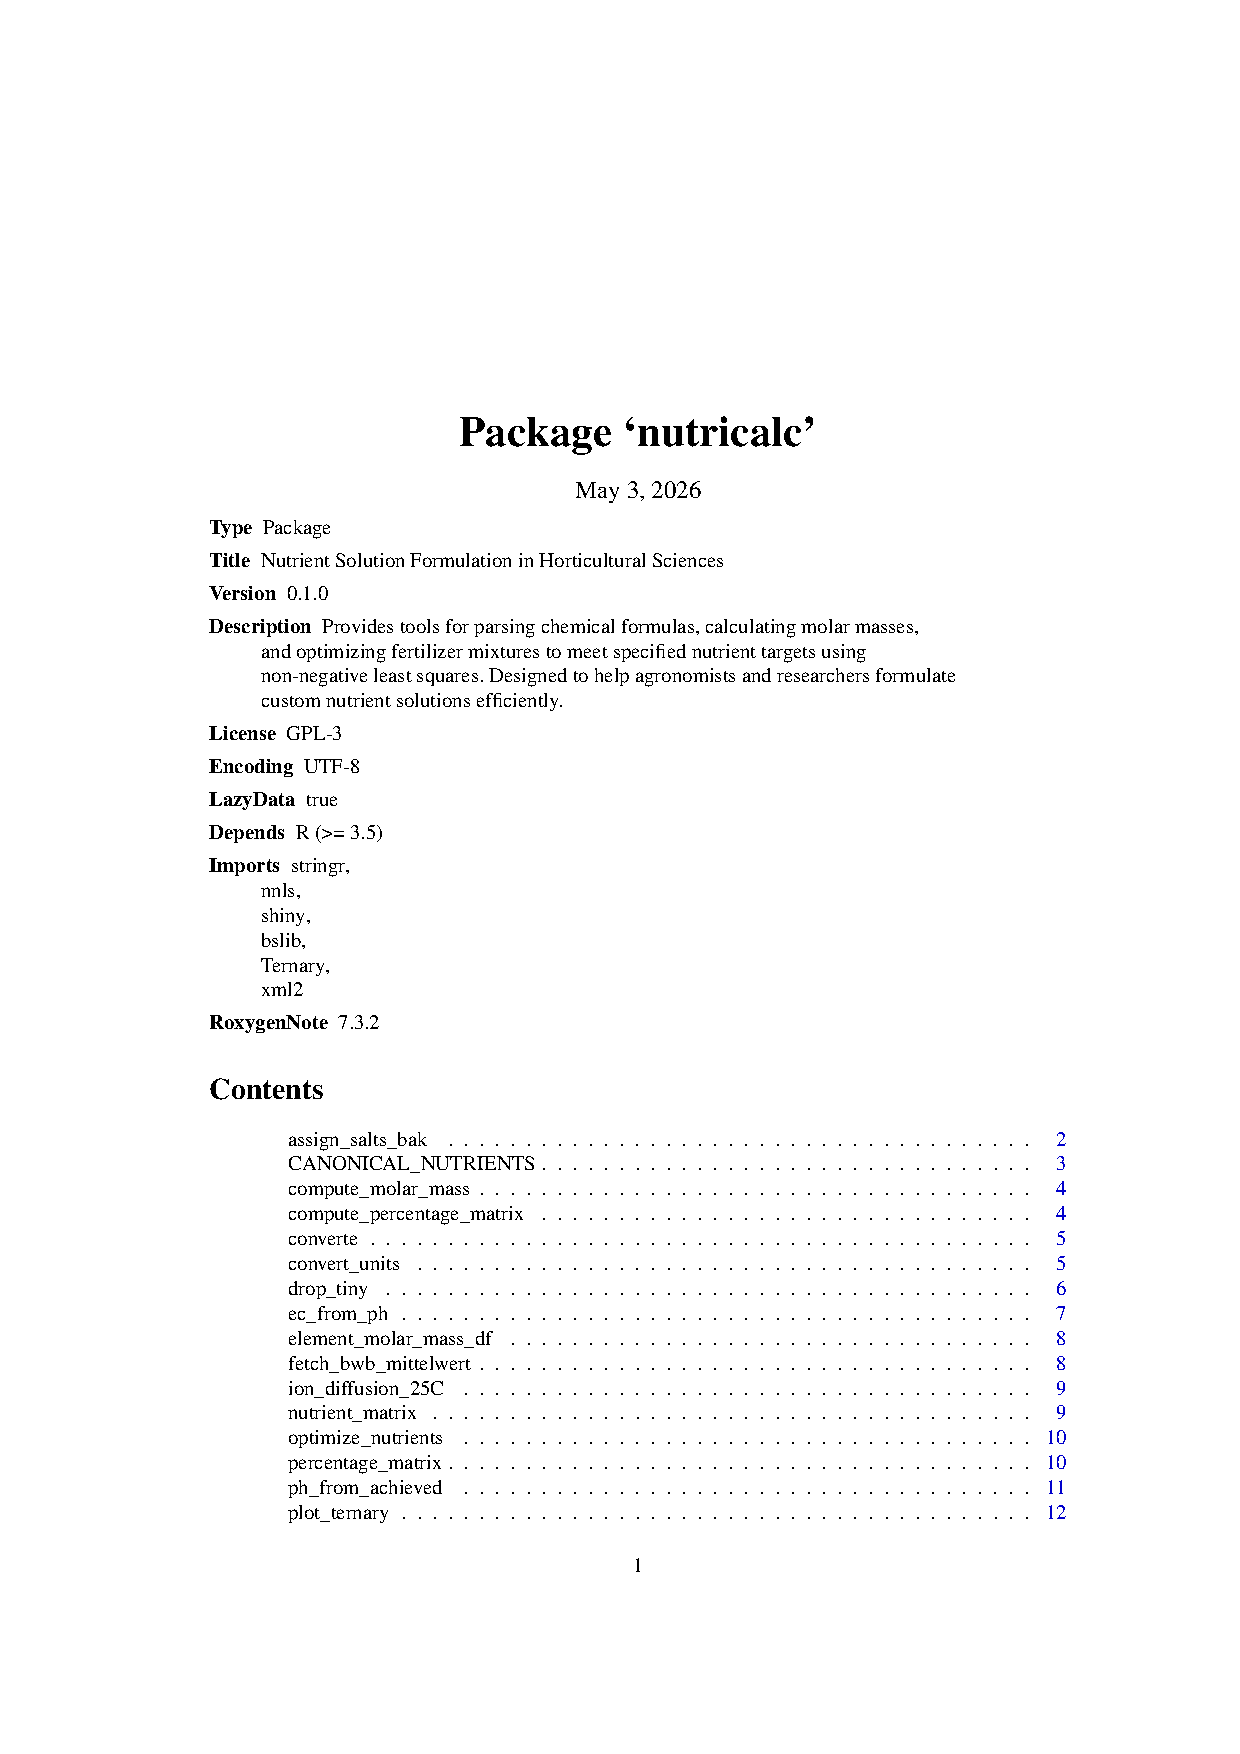
\includepdf[pages=-]{nutricalc_0.1.0.pdf}

\cleardoublepage
\phantomsection
\addcontentsline{toc}{chapter}{Declaration of Independence}
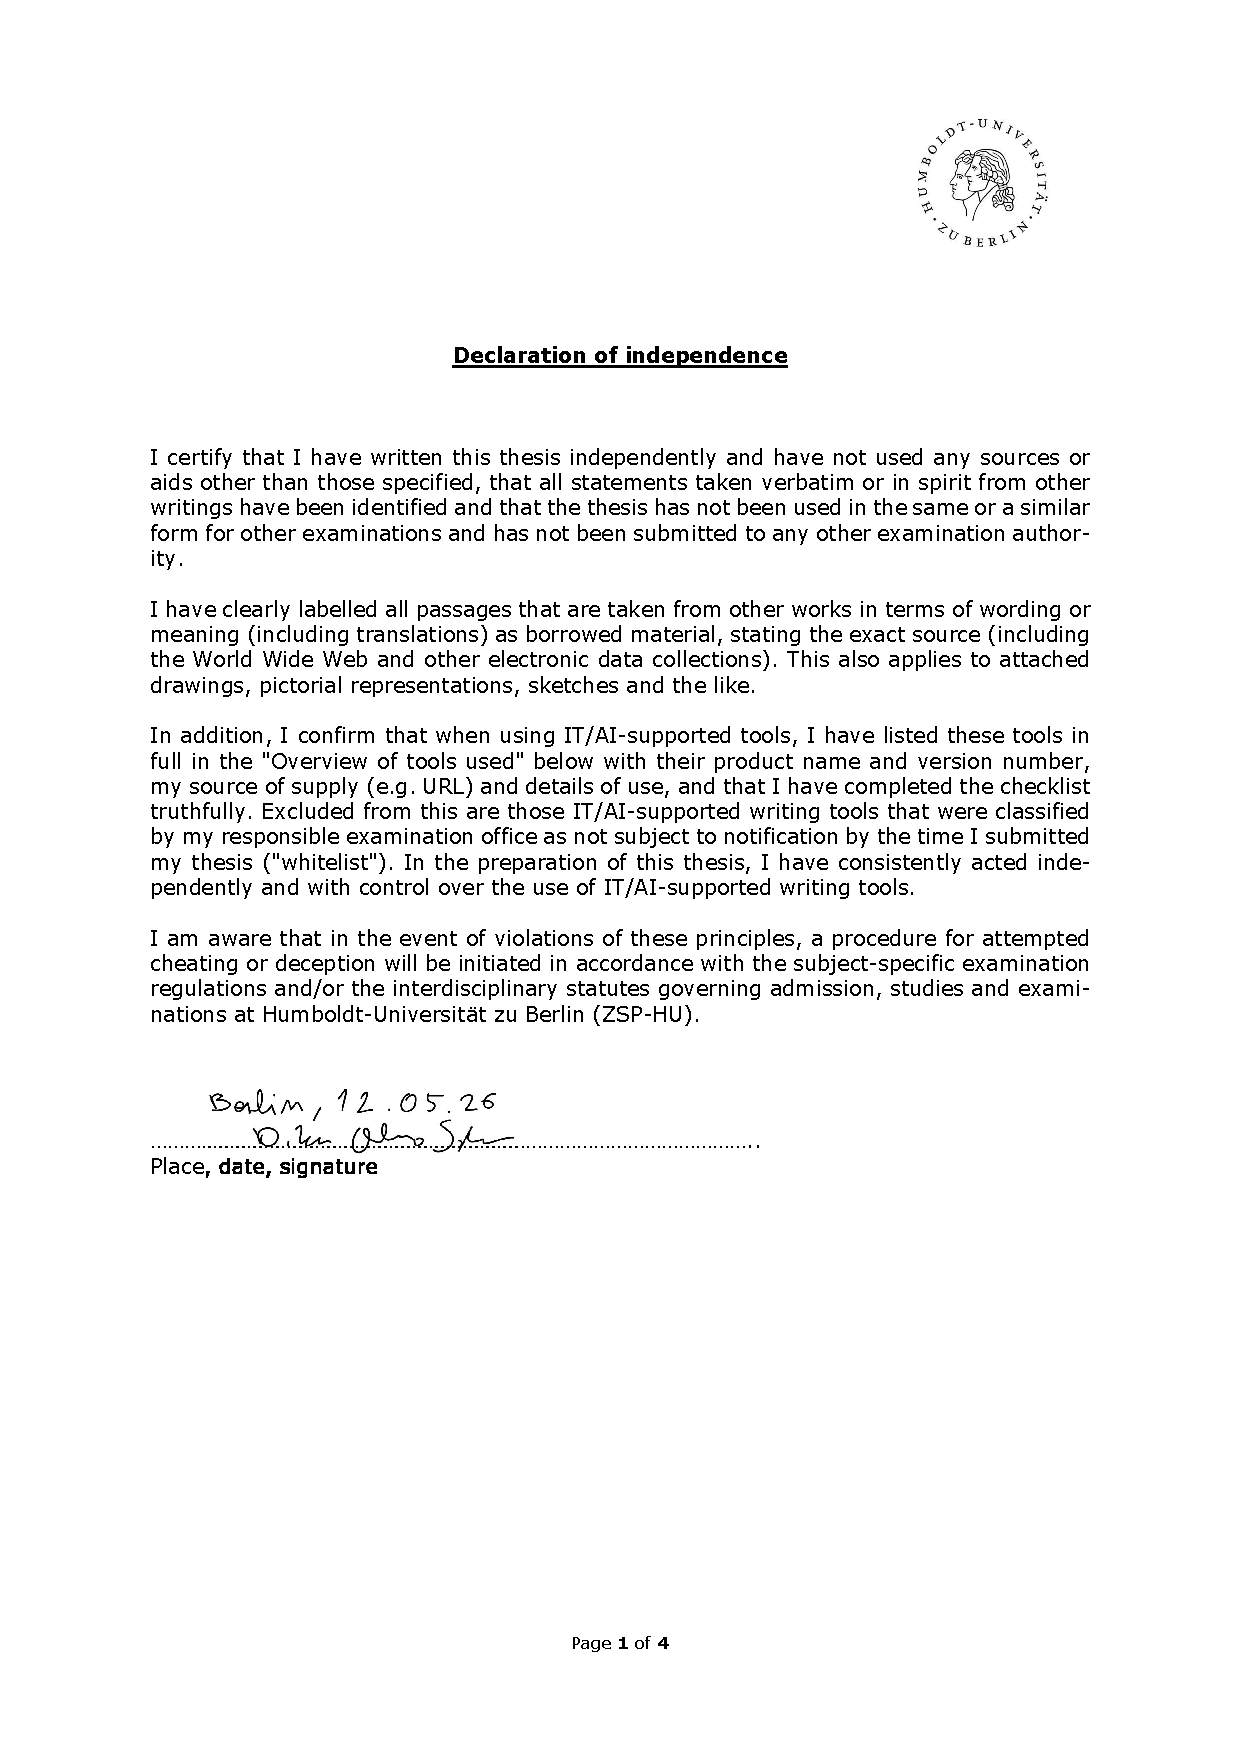
\includepdf[pages=-,pagecommand={}]{Declaration.pdf}




\end{document}
